% ******************************************************************************************
% A Classic Thesis Style
% An Homage to The Elements of Typographic Style
%
% Copyright (C) 2018 André Miede and Ivo Pletikosić
%
% If you like the style then I would appreciate a postcard. My address
% can be found in the file ClassicThesis.pdf. A collection of the
% postcards I received so far is available online at
% http://postcards.miede.de
%
% License:
% This program is free software; you can redistribute it and/or modify
% it under the terms of the GNU General Public License as published by
% the Free Software Foundation; either version 2 of the License, or
% (at your option) any later version.
%
% This program is distributed in the hope that it will be useful,
% but WITHOUT ANY WARRANTY; without even the implied warranty of
% MERCHANTABILITY or FITNESS FOR A PARTICULAR PURPOSE.  See the
% GNU General Public License for more details.
%
% You should have received a copy of the GNU General Public License
% along with this program; see the file COPYING.  If not, write to
% the Free Software Foundation, Inc., 59 Temple Place - Suite 330,
% Boston, MA 02111-1307, USA.
%
% PLEASE SEE ALSO THE AUTHORS' NOTE REGARDING THIS LICENSE
% IN THE DOCUMENTATION (ClassicThesis.pdf --> Chapter 1 / Chapter01.tex)
% ******************************************************************************************
\RequirePackage{silence} % :-\
    \WarningFilter{scrreprt}{Usage of package `titlesec'}
    %\WarningFilter{scrreprt}{Activating an ugly workaround}
    \WarningFilter{titlesec}{Non standard sectioning command detected}
\documentclass[ twoside,openright,titlepage,numbers=noenddot,%1headlines,
                headinclude,footinclude,cleardoublepage=empty,abstract=on,
                BCOR=5mm,paper=a4,fontsize=11pt
                ]{scrreprt}

%********************************************************************
% Note: Make all your adjustments in here
%*******************************************************
% ****************************************************************************************************
% classicthesis-config.tex
% formerly known as loadpackages.sty, classicthesis-ldpkg.sty, and classicthesis-preamble.sty
% Use it at the beginning of your ClassicThesis.tex, or as a LaTeX Preamble
% in your ClassicThesis.{tex,lyx} with % ****************************************************************************************************
% classicthesis-config.tex
% formerly known as loadpackages.sty, classicthesis-ldpkg.sty, and classicthesis-preamble.sty
% Use it at the beginning of your ClassicThesis.tex, or as a LaTeX Preamble
% in your ClassicThesis.{tex,lyx} with % ****************************************************************************************************
% classicthesis-config.tex
% formerly known as loadpackages.sty, classicthesis-ldpkg.sty, and classicthesis-preamble.sty
% Use it at the beginning of your ClassicThesis.tex, or as a LaTeX Preamble
% in your ClassicThesis.{tex,lyx} with \input{classicthesis-config}
% ****************************************************************************************************
% If you like the classicthesis, then I would appreciate a postcard.
% My address can be found in the file ClassicThesis.pdf. A collection
% of the postcards I received so far is available online at
% http://postcards.miede.de
% ****************************************************************************************************


% ****************************************************************************************************
% 0. Set the encoding of your files. UTF-8 is the only sensible encoding nowadays. If you can't read
% äöüßáéçèê∂åëæƒÏ€ then change the encoding setting in your editor, not the line below. If your editor
% does not support utf8 use another editor!
% ****************************************************************************************************
\PassOptionsToPackage{utf8}{inputenc}
  \usepackage{inputenc}

\PassOptionsToPackage{T1}{fontenc} % T2A for cyrillics
  \usepackage{fontenc}


% ****************************************************************************************************
% 1. Configure classicthesis for your needs here, e.g., remove "drafting" below
% in order to deactivate the time-stamp on the pages
% (see ClassicThesis.pdf for more information):
% ****************************************************************************************************
\PassOptionsToPackage{
  drafting=true,    % print version information on the bottom of the pages
  tocaligned=false, % the left column of the toc will be aligned (no indentation)
  dottedtoc=false,  % page numbers in ToC flushed right
  eulerchapternumbers=true, % use AMS Euler for chapter font (otherwise Palatino)
  linedheaders=false,       % chaper headers will have line above and beneath
  floatperchapter=true,     % numbering per chapter for all floats (i.e., Figure 1.1)
  eulermath=true,  % use awesome Euler fonts for mathematical formulae (only with pdfLaTeX)
  beramono=true,    % toggle a nice monospaced font (w/ bold)
  palatino=true,    % deactivate standard font for loading another one, see the last section at the end of this file for suggestions
  style=arsclassica % classicthesis, arsclassica
}{classicthesis}


% ****************************************************************************************************
% 2. Personal data and user ad-hoc commands (insert your own data here)
% ****************************************************************************************************
\newcommand{\myTitle}{Implementazione di un algoritmo KNN multiclasse su hardware quantistico\xspace}
\newcommand{\mySubtitle}{Classificazione multiclasse e costruzione di stati tramite QRAM\xspace}
\newcommand{\myDegree}{Laurea triennale\xspace}
\newcommand{\myName}{Mariano Mollo\xspace}
\newcommand{\myProf}{Giovanni Acampora\xspace}
\newcommand{\myOtherProf}{Autilia Vitiello\xspace}
\newcommand{\mySupervisor}{Put name here\xspace}
\newcommand{\myFaculty}{Scuola Politecnica e delle Scienze di Base\texorpdfstring{\\}{,}Area Didattica di Scienze Matematiche Fisiche e Naturali\xspace}
\newcommand{\myDepartment}{Dipartimento di Fisica "Ettore Pancini"\xspace}
\newcommand{\myUni}{Università degli Studi di Napoli "Federico II"\xspace}
\newcommand{\myLocation}{Napoli\xspace}
\newcommand{\myTime}{Ottobre 2019\xspace}
\newcommand{\myVersion}{\classicthesis}

\usepackage{braket}

\newcommand{\Id}{\ensuremath{\begin{pmatrix}
  1&0\\0&1
\end{pmatrix}}}

\usepackage{rotating}
\usepackage{adjustbox}
\usepackage{blindtext}
% \usepackage{natbib}
\usepackage{float}
% \usepackage{svg}

% ********************************************************************
% Setup, finetuning, and useful commands
% ********************************************************************
\providecommand{\mLyX}{L\kern-.1667em\lower.25em\hbox{Y}\kern-.125emX\@}
\newcommand{\ie}{i.\,e.}
\newcommand{\Ie}{I.\,e.}
\newcommand{\eg}{e.\,g.}
\newcommand{\Eg}{E.\,g.}
% ****************************************************************************************************


% ****************************************************************************************************
% 3. Loading some handy packages
% ****************************************************************************************************
% ********************************************************************
% Packages with options that might require adjustments
% ********************************************************************
\PassOptionsToPackage{english, italian}{babel} % change this to your language(s), main language last
% Spanish languages need extra options in order to work with this template
%\PassOptionsToPackage{spanish,es-lcroman}{babel}
    \usepackage{babel}

\usepackage{csquotes}
\PassOptionsToPackage{%
  %backend=biber,bibencoding=utf8, %instead of bibtex
  backend=bibtex8,bibencoding=ascii,%
  language=auto,%
  style=numeric-comp,%
  %style=authoryear-comp, % Author 1999, 2010
  %bibstyle=authoryear,dashed=false, % dashed: substitute rep. author with ---
  sorting=nyt, % name, year, title
  maxbibnames=10, % default: 3, et al.
  %backref=true,%
  natbib=true % natbib compatibility mode (\citep and \citet still work)
}{biblatex}
    \usepackage{biblatex}

\PassOptionsToPackage{fleqn}{amsmath}       % math environments and more by the AMS
  \usepackage{amsmath}

% ********************************************************************
% General useful packages
% ********************************************************************
\usepackage{graphicx} %
\usepackage{scrhack} % fix warnings when using KOMA with listings package
\usepackage{xspace} % to get the spacing after macros right
\PassOptionsToPackage{printonlyused,smaller}{acronym}
  \usepackage{acronym} % nice macros for handling all acronyms in the thesis
  %\renewcommand{\bflabel}[1]{{#1}\hfill} % fix the list of acronyms --> no longer working
  %\renewcommand*{\acsfont}[1]{\textsc{#1}}
  %\renewcommand*{\aclabelfont}[1]{\acsfont{#1}}
  %\def\bflabel#1{{#1\hfill}}
  \def\bflabel#1{{\acsfont{#1}\hfill}}
  \def\aclabelfont#1{\acsfont{#1}}
% ****************************************************************************************************
%\usepackage{pgfplots} % External TikZ/PGF support (thanks to Andreas Nautsch)
%\usetikzlibrary{external}
%\tikzexternalize[mode=list and make, prefix=ext-tikz/]
% ****************************************************************************************************


% ****************************************************************************************************
% 4. Setup floats: tables, (sub)figures, and captions
% ****************************************************************************************************
\usepackage{tabularx} % better tables
  \setlength{\extrarowheight}{3pt} % increase table row height
\newcommand{\tableheadline}[1]{\multicolumn{1}{l}{\spacedlowsmallcaps{#1}}}
\newcommand{\myfloatalign}{\centering} % to be used with each float for alignment
\usepackage{subfig}
% ****************************************************************************************************


% ****************************************************************************************************
% 5. Setup code listings
% ****************************************************************************************************
\usepackage{listings}
%\lstset{emph={trueIndex,root},emphstyle=\color{BlueViolet}}%\underbar} % for special keywords
\lstset{language=[LaTeX]Tex,%C++,
  morekeywords={PassOptionsToPackage,selectlanguage},
  keywordstyle=\color{RoyalBlue},%\bfseries,
  basicstyle=\small\ttfamily,
  %identifierstyle=\color{NavyBlue},
  commentstyle=\color{Green}\ttfamily,
  stringstyle=\rmfamily,
  numbers=none,%left,%
  numberstyle=\scriptsize,%\tiny
  stepnumber=5,
  numbersep=8pt,
  showstringspaces=false,
  breaklines=true,
  %frameround=ftff,
  %frame=single,
  belowcaptionskip=.75\baselineskip
  %frame=L
}
% ****************************************************************************************************




% ****************************************************************************************************
% 6. Last calls before the bar closes
% ****************************************************************************************************
% ********************************************************************
% Her Majesty herself
% ********************************************************************
\usepackage{classicthesis}


% ********************************************************************
% Fine-tune hyperreferences (hyperref should be called last)
% ********************************************************************
\hypersetup{%
  %draft, % hyperref's draft mode, for printing see below
  colorlinks=true, linktocpage=true, pdfstartpage=3, pdfstartview=FitV,%
  % uncomment the following line if you want to have black links (e.g., for printing)
  %colorlinks=false, linktocpage=false, pdfstartpage=3, pdfstartview=FitV, pdfborder={0 0 0},%
  breaklinks=true, pageanchor=true,%
  pdfpagemode=UseNone, %
  % pdfpagemode=UseOutlines,%
  plainpages=false, bookmarksnumbered, bookmarksopen=true, bookmarksopenlevel=1,%
  hypertexnames=true, pdfhighlight=/O,%nesting=true,%frenchlinks,%
  urlcolor=CTurl, linkcolor=CTlink, citecolor=CTcitation, %pagecolor=RoyalBlue,%
  %urlcolor=Black, linkcolor=Black, citecolor=Black, %pagecolor=Black,%
  pdftitle={\myTitle},%
  pdfauthor={\textcopyright\ \myName, \myUni, \myFaculty},%
  pdfsubject={},%
  pdfkeywords={},%
  pdfcreator={pdfLaTeX},%
  pdfproducer={LaTeX with hyperref and classicthesis}%
}


% ********************************************************************
% Setup autoreferences (hyperref and babel)
% ********************************************************************
% There are some issues regarding autorefnames
% http://www.tex.ac.uk/cgi-bin/texfaq2html?label=latexwords
% you have to redefine the macros for the
% language you use, e.g., american, ngerman
% (as chosen when loading babel/AtBeginDocument)
% ********************************************************************
\makeatletter
\@ifpackageloaded{babel}%
  {%
    \addto\extrasamerican{%
      \renewcommand*{\figureautorefname}{Figure}%
      \renewcommand*{\tableautorefname}{Table}%
      \renewcommand*{\partautorefname}{Part}%
      \renewcommand*{\chapterautorefname}{Chapter}%
      \renewcommand*{\sectionautorefname}{Section}%
      \renewcommand*{\subsectionautorefname}{Section}%
      \renewcommand*{\subsubsectionautorefname}{Section}%
    }%
    \addto\extrasngerman{%
      \renewcommand*{\paragraphautorefname}{Absatz}%
      \renewcommand*{\subparagraphautorefname}{Unterabsatz}%
      \renewcommand*{\footnoteautorefname}{Fu\"snote}%
      \renewcommand*{\FancyVerbLineautorefname}{Zeile}%
      \renewcommand*{\theoremautorefname}{Theorem}%
      \renewcommand*{\appendixautorefname}{Anhang}%
      \renewcommand*{\equationautorefname}{Gleichung}%
      \renewcommand*{\itemautorefname}{Punkt}%
    }%
      % Fix to getting autorefs for subfigures right (thanks to Belinda Vogt for changing the definition)
      \providecommand{\subfigureautorefname}{\figureautorefname}%
    }{\relax}
\makeatother


% ********************************************************************
% Development Stuff
% ********************************************************************
\listfiles
%\PassOptionsToPackage{l2tabu,orthodox,abort}{nag}
%  \usepackage{nag}
%\PassOptionsToPackage{warning, all}{onlyamsmath}
%  \usepackage{onlyamsmath}


% ****************************************************************************************************
% 7. Further adjustments (experimental)
% ****************************************************************************************************
% ********************************************************************
% Changing the text area
% ********************************************************************
%\areaset[current]{312pt}{761pt} % 686 (factor 2.2) + 33 head + 42 head \the\footskip
%\setlength{\marginparwidth}{7em}%
%\setlength{\marginparsep}{2em}%

% ********************************************************************
% Using different fonts
% ********************************************************************
%\usepackage[oldstylenums]{kpfonts} % oldstyle notextcomp
% \usepackage[osf]{libertine}
%\usepackage[light,condensed,math]{iwona}
%\renewcommand{\sfdefault}{iwona}
%\usepackage{lmodern} % <-- no osf support :-(
%\usepackage{cfr-lm} %
%\usepackage[urw-garamond]{mathdesign} <-- no osf support :-(
%\usepackage[default,osfigures]{opensans} % scale=0.95
%\usepackage[sfdefault]{FiraSans}
% \usepackage[opticals,mathlf]{MinionPro} % onlytext
% ********************************************************************
%\usepackage[largesc,osf]{newpxtext}
%\linespread{1.05} % a bit more for Palatino
% Used to fix these:
% https://bitbucket.org/amiede/classicthesis/issues/139/italics-in-pallatino-capitals-chapter
% https://bitbucket.org/amiede/classicthesis/issues/45/problema-testatine-su-classicthesis-style
% ********************************************************************
% ****************************************************************************************************

% ****************************************************************************************************
% If you like the classicthesis, then I would appreciate a postcard.
% My address can be found in the file ClassicThesis.pdf. A collection
% of the postcards I received so far is available online at
% http://postcards.miede.de
% ****************************************************************************************************


% ****************************************************************************************************
% 0. Set the encoding of your files. UTF-8 is the only sensible encoding nowadays. If you can't read
% äöüßáéçèê∂åëæƒÏ€ then change the encoding setting in your editor, not the line below. If your editor
% does not support utf8 use another editor!
% ****************************************************************************************************
\PassOptionsToPackage{utf8}{inputenc}
  \usepackage{inputenc}

\PassOptionsToPackage{T1}{fontenc} % T2A for cyrillics
  \usepackage{fontenc}


% ****************************************************************************************************
% 1. Configure classicthesis for your needs here, e.g., remove "drafting" below
% in order to deactivate the time-stamp on the pages
% (see ClassicThesis.pdf for more information):
% ****************************************************************************************************
\PassOptionsToPackage{
  drafting=true,    % print version information on the bottom of the pages
  tocaligned=false, % the left column of the toc will be aligned (no indentation)
  dottedtoc=false,  % page numbers in ToC flushed right
  eulerchapternumbers=true, % use AMS Euler for chapter font (otherwise Palatino)
  linedheaders=false,       % chaper headers will have line above and beneath
  floatperchapter=true,     % numbering per chapter for all floats (i.e., Figure 1.1)
  eulermath=true,  % use awesome Euler fonts for mathematical formulae (only with pdfLaTeX)
  beramono=true,    % toggle a nice monospaced font (w/ bold)
  palatino=true,    % deactivate standard font for loading another one, see the last section at the end of this file for suggestions
  style=arsclassica % classicthesis, arsclassica
}{classicthesis}


% ****************************************************************************************************
% 2. Personal data and user ad-hoc commands (insert your own data here)
% ****************************************************************************************************
\newcommand{\myTitle}{Implementazione di un algoritmo KNN multiclasse su hardware quantistico\xspace}
\newcommand{\mySubtitle}{Classificazione multiclasse e costruzione di stati tramite QRAM\xspace}
\newcommand{\myDegree}{Laurea triennale\xspace}
\newcommand{\myName}{Mariano Mollo\xspace}
\newcommand{\myProf}{Giovanni Acampora\xspace}
\newcommand{\myOtherProf}{Autilia Vitiello\xspace}
\newcommand{\mySupervisor}{Put name here\xspace}
\newcommand{\myFaculty}{Scuola Politecnica e delle Scienze di Base\texorpdfstring{\\}{,}Area Didattica di Scienze Matematiche Fisiche e Naturali\xspace}
\newcommand{\myDepartment}{Dipartimento di Fisica "Ettore Pancini"\xspace}
\newcommand{\myUni}{Università degli Studi di Napoli "Federico II"\xspace}
\newcommand{\myLocation}{Napoli\xspace}
\newcommand{\myTime}{Ottobre 2019\xspace}
\newcommand{\myVersion}{\classicthesis}

\usepackage{braket}

\newcommand{\Id}{\ensuremath{\begin{pmatrix}
  1&0\\0&1
\end{pmatrix}}}

\usepackage{rotating}
\usepackage{adjustbox}
\usepackage{blindtext}
% \usepackage{natbib}
\usepackage{float}
% \usepackage{svg}

% ********************************************************************
% Setup, finetuning, and useful commands
% ********************************************************************
\providecommand{\mLyX}{L\kern-.1667em\lower.25em\hbox{Y}\kern-.125emX\@}
\newcommand{\ie}{i.\,e.}
\newcommand{\Ie}{I.\,e.}
\newcommand{\eg}{e.\,g.}
\newcommand{\Eg}{E.\,g.}
% ****************************************************************************************************


% ****************************************************************************************************
% 3. Loading some handy packages
% ****************************************************************************************************
% ********************************************************************
% Packages with options that might require adjustments
% ********************************************************************
\PassOptionsToPackage{english, italian}{babel} % change this to your language(s), main language last
% Spanish languages need extra options in order to work with this template
%\PassOptionsToPackage{spanish,es-lcroman}{babel}
    \usepackage{babel}

\usepackage{csquotes}
\PassOptionsToPackage{%
  %backend=biber,bibencoding=utf8, %instead of bibtex
  backend=bibtex8,bibencoding=ascii,%
  language=auto,%
  style=numeric-comp,%
  %style=authoryear-comp, % Author 1999, 2010
  %bibstyle=authoryear,dashed=false, % dashed: substitute rep. author with ---
  sorting=nyt, % name, year, title
  maxbibnames=10, % default: 3, et al.
  %backref=true,%
  natbib=true % natbib compatibility mode (\citep and \citet still work)
}{biblatex}
    \usepackage{biblatex}

\PassOptionsToPackage{fleqn}{amsmath}       % math environments and more by the AMS
  \usepackage{amsmath}

% ********************************************************************
% General useful packages
% ********************************************************************
\usepackage{graphicx} %
\usepackage{scrhack} % fix warnings when using KOMA with listings package
\usepackage{xspace} % to get the spacing after macros right
\PassOptionsToPackage{printonlyused,smaller}{acronym}
  \usepackage{acronym} % nice macros for handling all acronyms in the thesis
  %\renewcommand{\bflabel}[1]{{#1}\hfill} % fix the list of acronyms --> no longer working
  %\renewcommand*{\acsfont}[1]{\textsc{#1}}
  %\renewcommand*{\aclabelfont}[1]{\acsfont{#1}}
  %\def\bflabel#1{{#1\hfill}}
  \def\bflabel#1{{\acsfont{#1}\hfill}}
  \def\aclabelfont#1{\acsfont{#1}}
% ****************************************************************************************************
%\usepackage{pgfplots} % External TikZ/PGF support (thanks to Andreas Nautsch)
%\usetikzlibrary{external}
%\tikzexternalize[mode=list and make, prefix=ext-tikz/]
% ****************************************************************************************************


% ****************************************************************************************************
% 4. Setup floats: tables, (sub)figures, and captions
% ****************************************************************************************************
\usepackage{tabularx} % better tables
  \setlength{\extrarowheight}{3pt} % increase table row height
\newcommand{\tableheadline}[1]{\multicolumn{1}{l}{\spacedlowsmallcaps{#1}}}
\newcommand{\myfloatalign}{\centering} % to be used with each float for alignment
\usepackage{subfig}
% ****************************************************************************************************


% ****************************************************************************************************
% 5. Setup code listings
% ****************************************************************************************************
\usepackage{listings}
%\lstset{emph={trueIndex,root},emphstyle=\color{BlueViolet}}%\underbar} % for special keywords
\lstset{language=[LaTeX]Tex,%C++,
  morekeywords={PassOptionsToPackage,selectlanguage},
  keywordstyle=\color{RoyalBlue},%\bfseries,
  basicstyle=\small\ttfamily,
  %identifierstyle=\color{NavyBlue},
  commentstyle=\color{Green}\ttfamily,
  stringstyle=\rmfamily,
  numbers=none,%left,%
  numberstyle=\scriptsize,%\tiny
  stepnumber=5,
  numbersep=8pt,
  showstringspaces=false,
  breaklines=true,
  %frameround=ftff,
  %frame=single,
  belowcaptionskip=.75\baselineskip
  %frame=L
}
% ****************************************************************************************************




% ****************************************************************************************************
% 6. Last calls before the bar closes
% ****************************************************************************************************
% ********************************************************************
% Her Majesty herself
% ********************************************************************
\usepackage{classicthesis}


% ********************************************************************
% Fine-tune hyperreferences (hyperref should be called last)
% ********************************************************************
\hypersetup{%
  %draft, % hyperref's draft mode, for printing see below
  colorlinks=true, linktocpage=true, pdfstartpage=3, pdfstartview=FitV,%
  % uncomment the following line if you want to have black links (e.g., for printing)
  %colorlinks=false, linktocpage=false, pdfstartpage=3, pdfstartview=FitV, pdfborder={0 0 0},%
  breaklinks=true, pageanchor=true,%
  pdfpagemode=UseNone, %
  % pdfpagemode=UseOutlines,%
  plainpages=false, bookmarksnumbered, bookmarksopen=true, bookmarksopenlevel=1,%
  hypertexnames=true, pdfhighlight=/O,%nesting=true,%frenchlinks,%
  urlcolor=CTurl, linkcolor=CTlink, citecolor=CTcitation, %pagecolor=RoyalBlue,%
  %urlcolor=Black, linkcolor=Black, citecolor=Black, %pagecolor=Black,%
  pdftitle={\myTitle},%
  pdfauthor={\textcopyright\ \myName, \myUni, \myFaculty},%
  pdfsubject={},%
  pdfkeywords={},%
  pdfcreator={pdfLaTeX},%
  pdfproducer={LaTeX with hyperref and classicthesis}%
}


% ********************************************************************
% Setup autoreferences (hyperref and babel)
% ********************************************************************
% There are some issues regarding autorefnames
% http://www.tex.ac.uk/cgi-bin/texfaq2html?label=latexwords
% you have to redefine the macros for the
% language you use, e.g., american, ngerman
% (as chosen when loading babel/AtBeginDocument)
% ********************************************************************
\makeatletter
\@ifpackageloaded{babel}%
  {%
    \addto\extrasamerican{%
      \renewcommand*{\figureautorefname}{Figure}%
      \renewcommand*{\tableautorefname}{Table}%
      \renewcommand*{\partautorefname}{Part}%
      \renewcommand*{\chapterautorefname}{Chapter}%
      \renewcommand*{\sectionautorefname}{Section}%
      \renewcommand*{\subsectionautorefname}{Section}%
      \renewcommand*{\subsubsectionautorefname}{Section}%
    }%
    \addto\extrasngerman{%
      \renewcommand*{\paragraphautorefname}{Absatz}%
      \renewcommand*{\subparagraphautorefname}{Unterabsatz}%
      \renewcommand*{\footnoteautorefname}{Fu\"snote}%
      \renewcommand*{\FancyVerbLineautorefname}{Zeile}%
      \renewcommand*{\theoremautorefname}{Theorem}%
      \renewcommand*{\appendixautorefname}{Anhang}%
      \renewcommand*{\equationautorefname}{Gleichung}%
      \renewcommand*{\itemautorefname}{Punkt}%
    }%
      % Fix to getting autorefs for subfigures right (thanks to Belinda Vogt for changing the definition)
      \providecommand{\subfigureautorefname}{\figureautorefname}%
    }{\relax}
\makeatother


% ********************************************************************
% Development Stuff
% ********************************************************************
\listfiles
%\PassOptionsToPackage{l2tabu,orthodox,abort}{nag}
%  \usepackage{nag}
%\PassOptionsToPackage{warning, all}{onlyamsmath}
%  \usepackage{onlyamsmath}


% ****************************************************************************************************
% 7. Further adjustments (experimental)
% ****************************************************************************************************
% ********************************************************************
% Changing the text area
% ********************************************************************
%\areaset[current]{312pt}{761pt} % 686 (factor 2.2) + 33 head + 42 head \the\footskip
%\setlength{\marginparwidth}{7em}%
%\setlength{\marginparsep}{2em}%

% ********************************************************************
% Using different fonts
% ********************************************************************
%\usepackage[oldstylenums]{kpfonts} % oldstyle notextcomp
% \usepackage[osf]{libertine}
%\usepackage[light,condensed,math]{iwona}
%\renewcommand{\sfdefault}{iwona}
%\usepackage{lmodern} % <-- no osf support :-(
%\usepackage{cfr-lm} %
%\usepackage[urw-garamond]{mathdesign} <-- no osf support :-(
%\usepackage[default,osfigures]{opensans} % scale=0.95
%\usepackage[sfdefault]{FiraSans}
% \usepackage[opticals,mathlf]{MinionPro} % onlytext
% ********************************************************************
%\usepackage[largesc,osf]{newpxtext}
%\linespread{1.05} % a bit more for Palatino
% Used to fix these:
% https://bitbucket.org/amiede/classicthesis/issues/139/italics-in-pallatino-capitals-chapter
% https://bitbucket.org/amiede/classicthesis/issues/45/problema-testatine-su-classicthesis-style
% ********************************************************************
% ****************************************************************************************************

% ****************************************************************************************************
% If you like the classicthesis, then I would appreciate a postcard.
% My address can be found in the file ClassicThesis.pdf. A collection
% of the postcards I received so far is available online at
% http://postcards.miede.de
% ****************************************************************************************************


% ****************************************************************************************************
% 0. Set the encoding of your files. UTF-8 is the only sensible encoding nowadays. If you can't read
% äöüßáéçèê∂åëæƒÏ€ then change the encoding setting in your editor, not the line below. If your editor
% does not support utf8 use another editor!
% ****************************************************************************************************
\PassOptionsToPackage{utf8}{inputenc}
  \usepackage{inputenc}

\PassOptionsToPackage{T1}{fontenc} % T2A for cyrillics
  \usepackage{fontenc}


% ****************************************************************************************************
% 1. Configure classicthesis for your needs here, e.g., remove "drafting" below
% in order to deactivate the time-stamp on the pages
% (see ClassicThesis.pdf for more information):
% ****************************************************************************************************
\PassOptionsToPackage{
  drafting=true,    % print version information on the bottom of the pages
  tocaligned=false, % the left column of the toc will be aligned (no indentation)
  dottedtoc=false,  % page numbers in ToC flushed right
  eulerchapternumbers=true, % use AMS Euler for chapter font (otherwise Palatino)
  linedheaders=false,       % chaper headers will have line above and beneath
  floatperchapter=true,     % numbering per chapter for all floats (i.e., Figure 1.1)
  eulermath=true,  % use awesome Euler fonts for mathematical formulae (only with pdfLaTeX)
  beramono=true,    % toggle a nice monospaced font (w/ bold)
  palatino=true,    % deactivate standard font for loading another one, see the last section at the end of this file for suggestions
  style=arsclassica % classicthesis, arsclassica
}{classicthesis}


% ****************************************************************************************************
% 2. Personal data and user ad-hoc commands (insert your own data here)
% ****************************************************************************************************
\newcommand{\myTitle}{Implementazione di un algoritmo KNN multiclasse su hardware quantistico\xspace}
\newcommand{\mySubtitle}{Classificazione multiclasse e costruzione di stati tramite QRAM\xspace}
\newcommand{\myDegree}{Laurea triennale\xspace}
\newcommand{\myName}{Mariano Mollo\xspace}
\newcommand{\myProf}{Giovanni Acampora\xspace}
\newcommand{\myOtherProf}{Autilia Vitiello\xspace}
\newcommand{\mySupervisor}{Put name here\xspace}
\newcommand{\myFaculty}{Scuola Politecnica e delle Scienze di Base\texorpdfstring{\\}{,}Area Didattica di Scienze Matematiche Fisiche e Naturali\xspace}
\newcommand{\myDepartment}{Dipartimento di Fisica "Ettore Pancini"\xspace}
\newcommand{\myUni}{Università degli Studi di Napoli "Federico II"\xspace}
\newcommand{\myLocation}{Napoli\xspace}
\newcommand{\myTime}{Ottobre 2019\xspace}
\newcommand{\myVersion}{\classicthesis}

\usepackage{braket}

\newcommand{\Id}{\ensuremath{\begin{pmatrix}
  1&0\\0&1
\end{pmatrix}}}

\usepackage{rotating}
\usepackage{adjustbox}
\usepackage{blindtext}
% \usepackage{natbib}
\usepackage{float}
% \usepackage{svg}

% ********************************************************************
% Setup, finetuning, and useful commands
% ********************************************************************
\providecommand{\mLyX}{L\kern-.1667em\lower.25em\hbox{Y}\kern-.125emX\@}
\newcommand{\ie}{i.\,e.}
\newcommand{\Ie}{I.\,e.}
\newcommand{\eg}{e.\,g.}
\newcommand{\Eg}{E.\,g.}
% ****************************************************************************************************


% ****************************************************************************************************
% 3. Loading some handy packages
% ****************************************************************************************************
% ********************************************************************
% Packages with options that might require adjustments
% ********************************************************************
\PassOptionsToPackage{english, italian}{babel} % change this to your language(s), main language last
% Spanish languages need extra options in order to work with this template
%\PassOptionsToPackage{spanish,es-lcroman}{babel}
    \usepackage{babel}

\usepackage{csquotes}
\PassOptionsToPackage{%
  %backend=biber,bibencoding=utf8, %instead of bibtex
  backend=bibtex8,bibencoding=ascii,%
  language=auto,%
  style=numeric-comp,%
  %style=authoryear-comp, % Author 1999, 2010
  %bibstyle=authoryear,dashed=false, % dashed: substitute rep. author with ---
  sorting=nyt, % name, year, title
  maxbibnames=10, % default: 3, et al.
  %backref=true,%
  natbib=true % natbib compatibility mode (\citep and \citet still work)
}{biblatex}
    \usepackage{biblatex}

\PassOptionsToPackage{fleqn}{amsmath}       % math environments and more by the AMS
  \usepackage{amsmath}

% ********************************************************************
% General useful packages
% ********************************************************************
\usepackage{graphicx} %
\usepackage{scrhack} % fix warnings when using KOMA with listings package
\usepackage{xspace} % to get the spacing after macros right
\PassOptionsToPackage{printonlyused,smaller}{acronym}
  \usepackage{acronym} % nice macros for handling all acronyms in the thesis
  %\renewcommand{\bflabel}[1]{{#1}\hfill} % fix the list of acronyms --> no longer working
  %\renewcommand*{\acsfont}[1]{\textsc{#1}}
  %\renewcommand*{\aclabelfont}[1]{\acsfont{#1}}
  %\def\bflabel#1{{#1\hfill}}
  \def\bflabel#1{{\acsfont{#1}\hfill}}
  \def\aclabelfont#1{\acsfont{#1}}
% ****************************************************************************************************
%\usepackage{pgfplots} % External TikZ/PGF support (thanks to Andreas Nautsch)
%\usetikzlibrary{external}
%\tikzexternalize[mode=list and make, prefix=ext-tikz/]
% ****************************************************************************************************


% ****************************************************************************************************
% 4. Setup floats: tables, (sub)figures, and captions
% ****************************************************************************************************
\usepackage{tabularx} % better tables
  \setlength{\extrarowheight}{3pt} % increase table row height
\newcommand{\tableheadline}[1]{\multicolumn{1}{l}{\spacedlowsmallcaps{#1}}}
\newcommand{\myfloatalign}{\centering} % to be used with each float for alignment
\usepackage{subfig}
% ****************************************************************************************************


% ****************************************************************************************************
% 5. Setup code listings
% ****************************************************************************************************
\usepackage{listings}
%\lstset{emph={trueIndex,root},emphstyle=\color{BlueViolet}}%\underbar} % for special keywords
\lstset{language=[LaTeX]Tex,%C++,
  morekeywords={PassOptionsToPackage,selectlanguage},
  keywordstyle=\color{RoyalBlue},%\bfseries,
  basicstyle=\small\ttfamily,
  %identifierstyle=\color{NavyBlue},
  commentstyle=\color{Green}\ttfamily,
  stringstyle=\rmfamily,
  numbers=none,%left,%
  numberstyle=\scriptsize,%\tiny
  stepnumber=5,
  numbersep=8pt,
  showstringspaces=false,
  breaklines=true,
  %frameround=ftff,
  %frame=single,
  belowcaptionskip=.75\baselineskip
  %frame=L
}
% ****************************************************************************************************




% ****************************************************************************************************
% 6. Last calls before the bar closes
% ****************************************************************************************************
% ********************************************************************
% Her Majesty herself
% ********************************************************************
\usepackage{classicthesis}


% ********************************************************************
% Fine-tune hyperreferences (hyperref should be called last)
% ********************************************************************
\hypersetup{%
  %draft, % hyperref's draft mode, for printing see below
  colorlinks=true, linktocpage=true, pdfstartpage=3, pdfstartview=FitV,%
  % uncomment the following line if you want to have black links (e.g., for printing)
  %colorlinks=false, linktocpage=false, pdfstartpage=3, pdfstartview=FitV, pdfborder={0 0 0},%
  breaklinks=true, pageanchor=true,%
  pdfpagemode=UseNone, %
  % pdfpagemode=UseOutlines,%
  plainpages=false, bookmarksnumbered, bookmarksopen=true, bookmarksopenlevel=1,%
  hypertexnames=true, pdfhighlight=/O,%nesting=true,%frenchlinks,%
  urlcolor=CTurl, linkcolor=CTlink, citecolor=CTcitation, %pagecolor=RoyalBlue,%
  %urlcolor=Black, linkcolor=Black, citecolor=Black, %pagecolor=Black,%
  pdftitle={\myTitle},%
  pdfauthor={\textcopyright\ \myName, \myUni, \myFaculty},%
  pdfsubject={},%
  pdfkeywords={},%
  pdfcreator={pdfLaTeX},%
  pdfproducer={LaTeX with hyperref and classicthesis}%
}


% ********************************************************************
% Setup autoreferences (hyperref and babel)
% ********************************************************************
% There are some issues regarding autorefnames
% http://www.tex.ac.uk/cgi-bin/texfaq2html?label=latexwords
% you have to redefine the macros for the
% language you use, e.g., american, ngerman
% (as chosen when loading babel/AtBeginDocument)
% ********************************************************************
\makeatletter
\@ifpackageloaded{babel}%
  {%
    \addto\extrasamerican{%
      \renewcommand*{\figureautorefname}{Figure}%
      \renewcommand*{\tableautorefname}{Table}%
      \renewcommand*{\partautorefname}{Part}%
      \renewcommand*{\chapterautorefname}{Chapter}%
      \renewcommand*{\sectionautorefname}{Section}%
      \renewcommand*{\subsectionautorefname}{Section}%
      \renewcommand*{\subsubsectionautorefname}{Section}%
    }%
    \addto\extrasngerman{%
      \renewcommand*{\paragraphautorefname}{Absatz}%
      \renewcommand*{\subparagraphautorefname}{Unterabsatz}%
      \renewcommand*{\footnoteautorefname}{Fu\"snote}%
      \renewcommand*{\FancyVerbLineautorefname}{Zeile}%
      \renewcommand*{\theoremautorefname}{Theorem}%
      \renewcommand*{\appendixautorefname}{Anhang}%
      \renewcommand*{\equationautorefname}{Gleichung}%
      \renewcommand*{\itemautorefname}{Punkt}%
    }%
      % Fix to getting autorefs for subfigures right (thanks to Belinda Vogt for changing the definition)
      \providecommand{\subfigureautorefname}{\figureautorefname}%
    }{\relax}
\makeatother


% ********************************************************************
% Development Stuff
% ********************************************************************
\listfiles
%\PassOptionsToPackage{l2tabu,orthodox,abort}{nag}
%  \usepackage{nag}
%\PassOptionsToPackage{warning, all}{onlyamsmath}
%  \usepackage{onlyamsmath}


% ****************************************************************************************************
% 7. Further adjustments (experimental)
% ****************************************************************************************************
% ********************************************************************
% Changing the text area
% ********************************************************************
%\areaset[current]{312pt}{761pt} % 686 (factor 2.2) + 33 head + 42 head \the\footskip
%\setlength{\marginparwidth}{7em}%
%\setlength{\marginparsep}{2em}%

% ********************************************************************
% Using different fonts
% ********************************************************************
%\usepackage[oldstylenums]{kpfonts} % oldstyle notextcomp
% \usepackage[osf]{libertine}
%\usepackage[light,condensed,math]{iwona}
%\renewcommand{\sfdefault}{iwona}
%\usepackage{lmodern} % <-- no osf support :-(
%\usepackage{cfr-lm} %
%\usepackage[urw-garamond]{mathdesign} <-- no osf support :-(
%\usepackage[default,osfigures]{opensans} % scale=0.95
%\usepackage[sfdefault]{FiraSans}
% \usepackage[opticals,mathlf]{MinionPro} % onlytext
% ********************************************************************
%\usepackage[largesc,osf]{newpxtext}
%\linespread{1.05} % a bit more for Palatino
% Used to fix these:
% https://bitbucket.org/amiede/classicthesis/issues/139/italics-in-pallatino-capitals-chapter
% https://bitbucket.org/amiede/classicthesis/issues/45/problema-testatine-su-classicthesis-style
% ********************************************************************
% ****************************************************************************************************


%********************************************************************
% Bibliographies
%*******************************************************
\addbibresource{Bibliography.bib}
\addbibresource[label=ownpubs]{AMiede_Publications.bib}

%********************************************************************
% Hyphenation
%*******************************************************
%\hyphenation{put special hyphenation here}

% ********************************************************************
% GO!GO!GO! MOVE IT!
%*******************************************************
\begin{document}
\frenchspacing
\raggedbottom
\selectlanguage{italian} % american ngerman
%\renewcommand*{\bibname}{new name}
%\setbibpreamble{}
\pagenumbering{roman}
\pagestyle{plain}
%********************************************************************
% Frontmatter
%*******************************************************
%*******************************************************
% Little Dirty Titlepage
%*******************************************************
\thispagestyle{empty}
%\pdfbookmark[1]{Titel}{title}
%*******************************************************
\begin{addmargin}[-1cm]{-3cm}
\begin{center}
    \spacedlowsmallcaps{\myName} \\ \medskip

    \begingroup
        \color{CTtitle}\spacedallcaps{\myTitle}
    \endgroup
\end{center}
\end{addmargin}
%*******************************************************
% Titlepage
%*******************************************************
\begin{titlepage}
    \begin{addmargin}[-1cm]{-3cm}

    \begin{center}
        {\Large {\textbf \myUni}}
    \end{center} 

    \begin{center}
    
\includegraphics[width=0.5\textwidth]{gfx/logo-federico-II-blu}
    \end{center}

        \begin{center}
            \textbf{Scuola Politecnica e delle Scienze di Base}
        \end{center}
        \begin{center}
            \textbf{Area Didattica di Scienze Matematiche Fisiche e Naturali}
        \end{center}
        \vspace{5pt}
        \begin{center}
            \textbf{Dipartimento di Fisica \textquotedblleft Ettore Pancini\textquotedblright}
        \end{center}
        \vspace{15pt}
        \begin{center}
            {{ \textit{Laurea Triennale in Fisica}}}
        \end{center}
        \vspace{40pt}

        \begin{center}
            \begingroup
            {\Large\spacedallcaps{\textbf{\myTitle}}}
            \endgroup
        \end{center}
        
        \vfill

        \vspace{25mm}
        \par
        \noindent
        \begin{minipage}[t]{0.47\textwidth}
            \textbf{Relatori:}\\
            \myProf\\
            \myOtherProf
        \end{minipage}
        \hfill
        \begin{minipage}[t]{0.47\textwidth}\raggedleft
            \textbf{Candidato:}\\
            Mariano Mollo\\
            Matr. N85000880
        \end{minipage}
        \vspace{5.5mm}
        \begin{center}
            {\large{\textbf{Anno Accademico 2019/2020}}}
        \end{center}
    \end{addmargin}
    \end{titlepage}
\thispagestyle{empty}

\hfill

\vfill

\noindent\myName: \textit{\myTitle,} \mySubtitle, %\myDegree,
\textcopyright\ \myTime

%\bigskip
%
%\noindent\spacedlowsmallcaps{Supervisors}: \\
%\myProf \\
%\myOtherProf \\
%\mySupervisor
%
%\medskip
%
%\noindent\spacedlowsmallcaps{Location}: \\
%\myLocation
%
%\medskip
%
%\noindent\spacedlowsmallcaps{Time Frame}: \\
%\myTime

% \cleardoublepage%*******************************************************
% Dedication
%*******************************************************
\thispagestyle{empty}
\phantomsection
\pdfbookmark[1]{Dedica}{Dedica}

\vspace*{3cm}

\begin{center}
    \emph{Ohana} means family. \\
    Family means nobody gets left behind, or forgotten. \\ \medskip
    --- Lilo \& Stitch
\end{center}

\medskip

\begin{center}
    Dedicato a Cotoletta, gattino carino. \\ \smallskip
    1939\,--\,2005
\end{center}

%\cleardoublepage\include{FrontBackmatter/Foreword}
\cleardoublepage%*******************************************************
% Abstract
%*******************************************************
%\renewcommand{\abstractname}{Abstract}
\pdfbookmark[1]{Sommario}{Sommario}
% \addcontentsline{toc}{chapter}{\tocEntry{Abstract}}
\begingroup
\let\clearpage\relax
\let\cleardoublepage\relax
\let\cleardoublepage\relax

\chapter*{Sommario}
%enuncia il problema
Il campo del quantum machine learning è tra gli ambiti di ricerca più 
promettenti per quanto riguarda il miglioramento dell'analisi dei big data. 
%perché il problema è un problema
I problemi predominanti con cui devono confrontarsi i computer classici sono i 
limiti di memoria e la capacità di elaborazione in tempi appropriati.
% frase sorprendente
Sfruttando le proprietà quantomeccaniche della materia, i computer quantistici 
possono veicolare nuove metodologie d'analisi dati. 
% consguenze della frase sorprendente
A tal fine si esplorano le possibilità offerte dall'implementazione di un algoritmo KNN, 
attraverso il kit di sviluppo software Qiskit e la piattaforma online IBM Q Experience. 

% ML, problemi del ML
% QML come aiuta
% Meno accento sui big data, giusto come conseguenza o in conclusione


\vfill

\begin{otherlanguage}{english}
\pdfbookmark[1]{Abstract}{Abstract}
\chapter*{Abstract}
Quantum Machine Learning is among the most anticipated fields when dealing 
with improvements in big data analysis. 
The main issues classical computers have to confront with are limits in memory 
and enormous computation times. 
Making use of quantum mechanical properties of matter, quantum computers can
spur the development of new methods to improve big data analysis. 
With that in mind, this thesis explores the capabilities of an implementation of a KNN 
algorithm, using the Qiskit software development kit and the online platform IBM Q Experience. 
\end{otherlanguage}

\endgroup

\vfill

%\cleardoublepage%*******************************************************
% Publications
%*******************************************************
\pdfbookmark[1]{Publications}{publications}
\chapter*{Publications}\graffito{This is just an early --~and currently ugly~-- test!}
This might come in handy for PhD theses: some ideas and figures have appeared previously in the following publications:

%\noindent Put your publications from the thesis here. The packages \texttt{multibib} or \texttt{bibtopic} etc. can be used to handle multiple different bibliographies in your document.

\begin{refsection}[ownpubs]
    \small
    \nocite{*} % is local to to the enclosing refsection
    \printbibliography[heading=none]
\end{refsection}

\emph{Attention}: This requires a separate run of \texttt{bibtex} for your \texttt{refsection}, \eg, \texttt{ClassicThesis1-blx} for this file. You might also use \texttt{biber} as the backend for \texttt{biblatex}. See also \url{http://tex.stackexchange.com/questions/128196/problem-with-refsection}.

\cleardoublepage%*******************************************************
% Acknowledgments
%*******************************************************
\pdfbookmark[1]{Ringraziamenti}{Ringraziamenti}

\begin{flushright}{\slshape
    We have seen that computer programming is an art, \\
    because it applies accumulated knowledge to the world, \\
    because it requires skill and ingenuity, and especially \\
    because it produces objects of beauty.} \\ \medskip
    --- \defcitealias{knuth:1974}{Donald E. Knuth}\citetalias{knuth:1974} \citep{knuth:1974}
\end{flushright}



\bigskip

\begingroup
\let\clearpage\relax
\let\cleardoublepage\relax
\let\cleardoublepage\relax
\chapter*{Ringraziamenti}

Regarding the typography and other help, many thanks go to Marco
Kuhlmann, Philipp Lehman, Lothar Schlesier, Jim Young, Lorenzo
Pantieri and Enrico Gregorio\footnote{Members of GuIT (Gruppo
Italiano Utilizzatori di \TeX\ e \LaTeX )}, J\"org Sommer,
Joachim K\"ostler, Daniel Gottschlag, Denis Aydin, Paride
Legovini, Steffen Prochnow, Nicolas Repp, Hinrich Harms,
Roland Winkler, Jörg Weber, Henri Menke, Claus Lahiri,
Clemens Niederberger, Stefano Bragaglia, Jörn Hees,
Scott Lowe, Dave Howcroft, Jos\'e M. Alcaide, David Carlisle,
Ulrike Fischer, Hugues de Lassus, Csaba Hajdu, Dave Howcroft,
and the whole \LaTeX-community for support, ideas and
some great software.

\bigskip

\noindent\emph{Regarding \mLyX}: The \mLyX\ port was intially done by
\emph{Nicholas Mariette} in March 2009 and continued by
\emph{Ivo Pletikosi\'c} in 2011. Thank you very much for your
work and for the contributions to the original style.


\endgroup

\cleardoublepage%*******************************************************
% Table of Contents
%*******************************************************
\pagestyle{scrheadings}
%\phantomsection
\pdfbookmark[1]{\contentsname}{tableofcontents}
\setcounter{tocdepth}{2} % <-- 2 includes up to subsections in the ToC
\setcounter{secnumdepth}{3} % <-- 3 numbers up to subsubsections
\manualmark
\markboth{\spacedlowsmallcaps{\contentsname}}{\spacedlowsmallcaps{\contentsname}}
\tableofcontents
\automark[section]{chapter}
\renewcommand{\chaptermark}[1]{\markboth{\spacedlowsmallcaps{#1}}{\spacedlowsmallcaps{#1}}}
\renewcommand{\sectionmark}[1]{\markright{\textsc{\thesection}\enspace\spacedlowsmallcaps{#1}}}
%*******************************************************
% List of Figures and of the Tables
%*******************************************************
\clearpage
% \pagestyle{empty} % Uncomment this line if your lists should not have any headlines with section name and page number
\begingroup
    \let\clearpage\relax
    \let\cleardoublepage\relax
    %*******************************************************
    % List of Figures
    %*******************************************************
    %\phantomsection
    %\addcontentsline{toc}{chapter}{\listfigurename}
    \pdfbookmark[1]{\listfigurename}{lof}
    \listoffigures

    \vspace{8ex}

    %*******************************************************
    % List of Tables
    %*******************************************************
    %\phantomsection
    %\addcontentsline{toc}{chapter}{\listtablename}
    \pdfbookmark[1]{\listtablename}{lot}
    \listoftables

    \vspace{8ex}
    % \newpage

    %*******************************************************
    % List of Listings
    %*******************************************************
    %\phantomsection
    %\addcontentsline{toc}{chapter}{\lstlistlistingname}
    %https://tex.stackexchange.com/questions/64839/how-to-change-listing-caption
    \renewcommand{\lstlistingname}{Algoritmo}% Listing -> Algoritmo
    \renewcommand{\lstlistlistingname}{Elenco degli algoritmi}% List of Listings -> List of Algorithms
    \pdfbookmark[1]{\lstlistlistingname}{lol}
    \lstlistoflistings

    \vspace{8ex}

    %*******************************************************
    % Acronyms
    %*******************************************************
    %\phantomsection
    \pdfbookmark[1]{Acronimi}{Acronimi}
    \markboth{\spacedlowsmallcaps{Acronimi}}{\spacedlowsmallcaps{Acronimi}}
    \chapter*{Acronimi}
    \begin{acronym}[UMLX]
        \acro{DRY}{Don't Repeat Yourself}
        \acro{ML}{machine learning}
        \acro{CQ}{computer quantistico}
        \acro{QC}{quantum computer}
        \acro{MLQ}{machine learning quantistico}
        \acro{QML}{quantum machine learning}
        \acro{QRAM}{quantum random access memory}
        \acro{KNN}{k-nearest neighbours}
        \acro{FF-QRAM}{flip-flop QRAM}
        \acro{QDB}{quantum database}
    \end{acronym}

\endgroup

%********************************************************************
% Mainmatter
%*******************************************************
\cleardoublepage
\pagestyle{scrheadings}
\pagenumbering{arabic}
%\setcounter{page}{90}
% use \cleardoublepage here to avoid problems with pdfbookmark
\cleardoublepage
\ctparttext{Introduzione al campo del quantum computing e del quantum 
machine learning, presentazione della teoria di base e degli strumenti usati.}
\part{Teoria}\label{pt:presentazione}
%************************************************
\chapter{Introduzione}\label{ch:introduzione}
%************************************************

% L'abilità di riconoscere modelli da parte delle macchine è una cosa molto bella. 
% Per aiutare i computer dei nostri giorni che non ce la fanno più, si stanno ideando 
% varie soluzioni. Qui parlo dei computer quantistici, che sfruttano proprietà 
% della materia quando è molto fredda, che ci permettono di fare cose strabilianti. 

% L'articolo con cui è partita la mia attività di tesi è quello di Tacchino, 
% in cui implementa un percettrone a due qubit, che è capace di riconoscere 
% motivi a quattro bit. Quello su cui mi concentro io è un algoritmo analogo 
% e ugualmente semplice, detto k-Nearest Neighbour, ovvero i k vicini più vicini. 

% Per affrontare l'argomento sono partito dalla tesi di Mark Fingerhuth, che 
% ha implementato un algoritmo ma non è riuscito a farlo girare su un vero 
% computer quantistico, perché non ce n'erano ancora di abbastanza potenti. 
% Adesso ci sono, e ci divertiamo. 

%****************************************

Chiunque abbia un cellulare di nuova generazione è venuto in contatto con il 
campo del machine learning, la disciplina che si pone l'obiettivo di rendere 
i computer capaci di apprendere dall'esperienza. 
Gli esseri umani sono strettamente legati al processo di apprendimento, a 
partire dalla prima infanzia ed in maniera più o meno evidente durante 
tutto il corso vitale. 
Sebbene tale processo sembri automatico, in realtà è espressione di un 
complesso sistema di feedback, che in fin dei conti è codificato dal 
nostro codice genetico. 
Il \ac{ML} (tradotto \emph{apprendimento automatico}) prevede la scrittura 
del codice di programmazione che permetta 
ai computer di effettuare qualcosa di analogo all'apprendimento. 
\marginpar{Un esempio recente di uso del \ac{ML} è la funzione di gestione adattiva della batteria, 
lanciata in Android 9, che usa il machine learning per predire quali applicazioni 
l'utente userà nelle prossime ore e quali no, in modo da dedicare la carica solo per le 
applicazioni più usate dal proprietario. \cite{android10}}
Tali algoritmi sono il motore dei moderni assistenti vocali e dei sistemi 
che ci suggeriscono nuovi prodotti da acquistare o video da guardare, ma anche 
nel prevenire le frodi su carta di credito, per filtrare lo spam dalle nostre caselle 
email, nell'individuare e diagnosticare malattie, e tanto ancora \cite{pml}. 

% L'abilità di riconoscere facce familiari, di comprendere il linguaggio parlato e di 
% distinguere tra tipi di piante viene naturale agli esseri umani, sebbene
% % sebbene, benché, quantunque, anche se
% questi processi di riconoscimento di modelli e di classificazione siano intrinsecamente 
% complessi. Il \ac{ML}, una sottodisciplina dell'intelligenza artificiale, 
% si occupa dello sviluppo di algoritmi che eseguono questo tipo di compiti, permettendo 
% in questo modo % così
% ai computer di trovare e riconoscere modelli nei dati e di classificare input 
% % dati da elaborare
% sconosciuti % ignoti
% basandosi sui % in base ai
% precedenti dati di addestramento. % allenamento, ammaestramento
% Tali algoritmi formano il nucleo di p.e. motori di riconoscimento del linguaggio % parola
% umano e di raccomandazione come quelli usati da Amazon. % Fonti

Stando all'IBM \cite{ibm-big-data}, ogni giorno vengono creati circa $2,5\times10^{18}$ byte di dati: 
questo numero in costante crescita mette chi ha a che fare con i dati di fronte 
alla necessità di dotarsi di algoritmi avanzati che possando fare ordine in questo 
oceano di informazioni. Per trovare modelli e correlazioni su insiemi molto grandi
è necessario un numero di operazioni che richiede molto tempo ed 
energia per essere portate a termine; trovare metodi efficienti per completare 
questi compiti diventa necessario sotto molti punti di vista. 

Diversi lavori hanno evidenziato il ruolo nodale rispetto a questo problema 
che può avere l'uso della computazione quantistica, 
oggetto di intensa ricerca teorica da vari decenni 
e recentemente di sperimentazione da parte di studenti \cite{fingerhuth} e ricercatori \cite{schuld}. 

Un \ac{CQ} (o \ac{QC}) usa le proprietà peculiari dei sistemi quantomeccanici per manipolare 
ed elaborare l'informazione in modi inaccessibili ai normali computer classici. 
Così come un computer classico manipola bit, un computer quantistico fa uso dei 
cosiddetti bit quantistici (qubit). I bit e i qubit sono entrambi entità binarie, 
il che significa che possono assumere solo i valori 0 o 1. Ad ogni modo, un bit 
classico non probabilistico\footnote{Per informazioni sui bit classici 
probabilitici si faccia riferimento alla sezione 3.2 di \cite{mannucci}.} 
può assumere solo uno di questi valori alla volta, 
laddove un qubit può trovarsi in una sovrapposizione lineare dei due stati. 
Il fatto di lavorare con una sovrapposizione di stati di un sistema, 
invece che con uno stato definito alla volta, implica che si possono effettuare 
determinate operazioni che coinvolgono più stati contemporaneamente. 
% Questa possibilità è entusiasmante, ma di fronte a nuovi modi di 
% agire, si rende necessario sviluppare nuovi algoritmi e strategie di sviluppo. 

% "Stai pensando troppo classicamente"

Nonostante ciò, uno degli ostacoli principali di questo campo è rappresentato proprio dalla 
caratteristica alla base della meccanica quantistica: quando si ha un qubit 
in una sovrapposizione di stati, non possiamo conoscerne i dettagli intrinseci 
in un determinato istante, a meno di effettuare una misura; se ci provassimo, 
otterremmo un risultato ben definito, facendo collassare la funzione d'onda 
che descrive il qubit, riducendolo in fin dei conti ad un bit con uno stato definito (esattamente 
quello che misuriamo), e perdendo tutte le informazioni quantistiche 
contenute nel qubit. 

% Il tentativo negli ultimi anni è stato quello di costruire macchine 
% che sfruttassero queste proprietà a proprio vantaggio, a patto di obbedire 
% alle regole del gioco. Quando abbiamo un qubit in una sovrapposizione di 
% stati, non possiamo conoscere in quale stato si trovi in un determinato istante; 
% se ci provassimo, misurandolo, otterremmo un risultato ben definito, ma lo 
% avremmo fatto collassare e distrutto tutte le informazioni quantistiche che 
% conteneva. 

Per avere un'idea di come un \ac{CQ} si rapporti con un computer ordinario, 
si possono considerare diversi algoritmi quantistici, che forniscono 
accelerazioni esponenziali se confrontati con le loro controparti classiche; 
l'algoritmo di fattorizzazione in numeri primi di Shor è uno tra i più famosi \cite{shor}. 
% La computazione quantistica ha il potenziale di migliorare la potenza computazionale, 
% accelerare l'elaborazione di grandi dati e probabilmente risolvere alcuni problemi che sono 
% praticamente irrisolvibili su computer classici, p.e. problemi di ottimizzazione 
% computazionalmente dispendiosi come il ben noto problema del commesso viaggiatore con più 
% di 1000 città. % Fonti

% adesso è già avviata la combinazione tra ML e QC

Alla luce di questi fatti, negli ultimi anni c'è stata particolare attenzione nei 
riguardi del nuovo campo del \ac{MLQ} (o \ac{QML}) \cite{Biamonte2017} , che mette insieme il 
\ac{ML} con il quantum computing. 

Più nello specifico, si parla di machine learning migliorato quantisticamente quando 
la computazione quantistica è usata per migliorare algoritmi di \ac{ML} classico. 
Cionondimeno, entrambi i campi sono benefici l'un l'altro, 
poiché il \ac{ML} classico può anche essere usato per migliorare aspetti 
della computazione quantistica \cite{PhysRevLett.116.230504}. 
% Per esempio, Las Heras, Alvarez-Rodriguez, Solano e Sanz % Fonti
% hanno mostrato che un algoritmo genetico classico può essere usato per ridurre 
% l'errore sperimentale nelle porte logiche quantistiche. 
Questa tesi si occuperà solo del campo del machine 
learning aumentato quantisticamente. 

% ***********************************************

\section{Motivazione}

Il \ac{QML} è un campo molto giovane e in fermento. Stiamo assistendo a qualcosa di 
analogo a quella che era la nascita dei computer classici, ovvero lo sviluppo di un 
numero sempre crescente di algoritmi, tecniche ed hardware di base in 
un ambiente in cui le cose consolidate sono ben poche: il \ac{QML} è solo una 
delle branche che sono state reputate promettenti per quanto riguarda i vantaggi 
portati dai computer quantistici \cite{what-is-ibm-q}. \marginpar{I campi che si 
prevede otterranno accelerazioni maggiori grazie al quantum computing sono il 
machine learning, la simulazione di sistemi quantomeccanici, i problemi di 
ottimizzazione e l'analisi finanziaria.}
In ogni caso c'è necessità di inventare nuove strategie per risolvere anche i 
problemi più semplici: per avere risultati affidabili spesso si richiede un 
numero considerevole di qubit ed unità di memorizzazione che possano conservare 
informazioni quantistiche, come la \ac{QRAM}. 
Al giorno d'oggi il numero massimo di qubit a superconduzione, da quanto viene 
riferito, è di 50 \cite{50qubit}. 

Negli ultimi anni ci sono state varie implementazioni innovative di algoritmi di \ac{MLQ} \cite{quantum-advantage}: 
seguendo i passi che hanno portato alla nascita del \ac{ML} nel XX secolo, 
Tacchino et al. \cite{tacchino} hanno implementato un percettrone su hardware quantistico;
Schuld et al. \cite{schuld} hanno invece implementato l'algoritmo lazy learner \ac{KNN}. 
Questa tesi parte proprio da quest'ultimo articolo, provando a riprodurne il lavoro e ad 
implementarne una versione multiclasse. 

% Li, Liu, Xu e Du hanno distinto con successo cifre scritte a mano usando un quantum support 
% vector machine su un banco di prova a risonanza magnetica nucleare con quattro qubit. In più, 
% Cai et al. sono stati i primi a dimostrare sperimentalmente il machine learning quantistico su 
% un \ac{CQ} fotonico e hanno mostrato che la distanza tra due vettori e il loro prodotto 
% interno possono effettivamente essere computati quantomeccanicamente. 
% Infine, Ristè et al. hanno risolto un problema di learning parity con cinque qubit 
% superconduttivi e hanno trovato che un vantaggio quantistico può già essere osservato 
% in sistemi senza correzione degli errori. 

% Considerando il distacco tra il numero di algoritmi di \ac{MLQ} e le poche realizzazioni 
% sperimentali, considerando inoltre i recenti sviluppi nell'hardware quantistico, diventa 
% importante scoprire come i problemi di \ac{MLQ} realizzati di \ac{CQ} di piccola dimensione 
% scalino quando implementati su \ac{CQ} con maggiori risorse. 
% Di qui, l'obiettivo di questa ricerca è il fornire implementazioni come prova di principio, 
% simulazioni e risultati sperimentali di algoritmi di \ac{MLQ} selezionati a partire da 
% insiemi di dati di grandezza da piccola a media, osservando come cambiano i requisiti ed 
% i risultati passando da un caso all'altro. A questo scopo, l'algoritmo \acf{KNN}, uno tra i 
% più semplici algoritmi di \ac{ML}, è stato scelto come buon esempio minimale per 
% l'implementazione, la simulazione e la sperimentazione quantistica. 
% Questo è un passo necessario nel tentativo di far passare il \ac{MLQ} da un ambito di 
% ricerca quasi puramente teorico ad un campo più applicativo come è il \ac{ML} classico. 

% Il \ac{ML} classico è un ambito molto concreto poiché può essere direttamente testato, 
% verificato e implementato su qualsiasi computer classico commerciale. 
% Fino ad ora, il \ac{MLQ} è stato per la gran parte di natura teorica, dato che le risorse 
% computazionali richieste sono solo parzialmente sviluppate. Per produrre soluzioni affidabili, 
% gli algoritmi di \ac{MLQ} spesso richiedono un numero enorme di qubit con correzione 
% degli errori e qualche sistema di memorizzazione di dati quantistici, per esempio la 
% \ac{QRAM} proposta da Giovannetti, Lloyd e Maccone. % Fonti
% Io ho usato quella proposta da Petruccione, devo vedere se inserire il riferimento al posto 
% di questo o introdurlo dopo nel discorso

% Al giorno d'oggi il massimo numero di qubit p.e. a superconduzione, da quanto 
% viene riferito, usati per il calcolo sono quattordici; 
% si intende quelli a disposizione pubblica, poi il massimo al mondo bisogna verificarlo
% il D-Wave II quantum annealing device fornisce 1152 qubit ma può risolvere solo una ristretta 
% classe di problemi, e una \ac{QRAM} dedicata non è stata ancora sviluppata. % Fonti
% Verificare che sia ancora così
% Inoltre, la correzione degli errori dei qubit è un campo di ricerca ancora attivo 
% e sebbene ci siano stati notevoli miglioramenti, % mettere nota a margine con dati del miglioramento
% la maggior parte dei \ac{CQ} preliminari descritti hanno a che fare con qubit senza correzione 
% d'errore, con vite brevi e sono, quindi, inadatti per grandi implementazioni di \ac{MLQ}. 

\section{Domanda di ricerca}

% Alla luce della natura teorica dell'attuale ricerca nel \ac{MLQ} 
% e del piccolo numero di realizzazioni sperimentali, questa ricerca si dedicherà 
% alla seguente domanda: 
Prendendo come punto di partenza gli algoritmi proposti nell'ambito di ricerca del \ac{QML} 
questa tesi proverà a rispondere alla seguente domanda:
\begin{quote}
    è possibile implementare su un computer quantistico un algoritmo k-nearest neighbours 
    multiclasse, in modo da migliorare le prestazioni ed il numero di problemi risolvibili?
    % quali sono le prestazioni di un algoritmo k-nearest neighbours di quantum 
    % machine learning implementato su hadware quantistico di piccola e media dimensione 
    % attualmente disponibili e come scala all'aumentare delle risorse?
    % quali sono le opportunità di implementazione pratica e l'efficienza di un algoritmo 
    % k-nearest neighbours di machine learning quantistico su computer quantistici di piccola 
    % e media scala attualmente disponibili?
\end{quote}
I capitoli seguenti introdurranno le basi teoriche necessarie e gli strumenti usati 
per rispondere a questa domanda. 

%*****************************************
%*****************************************
%*****************************************
%*****************************************
%*****************************************

%************************************************
\chapter{Quantum computing e machine learning}\label{ch:teoria}
%************************************************

% \emph{
%     Si noti che tutti i concetti introdotti nelle sezioni 2.1 e 2.2 possono essere trovati in 
%     qualunque libro di testo di base sull'informazione quantistica e quindi non ci saranno 
%     riferimenti individuali ad essi. Entrambe queste sezioni sono principalmente basate sul libro 
%     di testo di Noson e Mannucci\cite{noson}.
% }

Nella sezione \ref{sec:quantum_computing} si discuteranno i concetti fondamentali su 
cui si base il funzionamento di un quantum computer. 
L'unità di base di un computer classico è il bit e l'unità di base di 
un computer quantistico è una generalizzazione del concetto di bit, 
chiamato qubit, che sarà discussa in sezione \ref{sec:qubit}. 
Nella sezione \ref{sec:porte_quantistiche} si presentano le porte 
logiche quantistiche, che permettono di manipolare i qubit. 
Infine, in sezione \ref{sec:decoerenza} si discuterà di uno dei nuovi problemi con 
cui si deve avere a che fare quando si lavora con oggetti quantomeccanici, ovvero 
la decoerenza. 

Successivamente, in sezione \ref{sec:machine_learning}, verrà introdotta brevemente 
la branca del machine learning, spiegando il funzionamento dell'algoritmo k-nearest neighbours, 
per poi discuterne la versione quantistica in sezione \ref{sec:qml}. 

\section{Quantum computing} \label{sec:quantum_computing}

\subsection{Bit e qubit} \label{sec:qubit}

\begin{definition}
    Un bit è un'unità di informazione che descrive un sistema classico 
    bidimensionale. 
\end{definition}
I due possibili stati di un bit sono generalmente scritti come 
0 e 1, o meglio, nel nostro caso $\ket{0}$ e $\ket{1}$. 
Usando una notazione matriciale, possiamo rappresentare questi due 
stati come 
\begin{equation}
    \ket{0} = \begin{matrix}
        0 \\ 1
    \end{matrix}
    \begin{pmatrix}
        1 \\ 0
    \end{pmatrix}, \quad
    \ket{1} = \begin{matrix}
        0 \\ 1
    \end{matrix}
    \begin{pmatrix}
        0 \\ 1
    \end{pmatrix},
\end{equation}
dove i numeri a margine delle matrici indicano a quale stato si 
riferisce un determinato elemento di base. Poiché queste due 
rappresentazioni sono ortogonali, abbiamo che il bit che 
può trovarsi in uno stato tra $\ket{0}$ e $\ket{1}$. 

\begin{definition}
    Un bit quantistico o qubit è un'unità di informazione che descrive 
    un sistema quantistico bidimensionale. 
\end{definition}
Si rappresenterà il qubit come una matrice $2\times1$ a valori complessi 
\begin{equation}
    \begin{matrix}
        0 \\ 1
    \end{matrix}
    \begin{pmatrix}
        c_0 \\ c_1
    \end{pmatrix},
\end{equation}
dove $|c_0|^2 + |c_1|^2 = 1$. Si noti che un bit classico è un caso particolare 
di qubit. $|c_0|^2$ va interpretata come la probabilità che dopo una misura del 
qubit, questo sarà trovato nello stato $\ket{0}$. $|c_1|^2$ va interpretata come 
la probabilità che dopo una misura del qubit, questo sarà trovato nello stato 
$\ket{1}$. Allorquando si misura lo stato di un qubit, questo diventa automaticamente 
un bit. Quindi non "vedremo" mai un qubit generico. Nonostante ciò, essi esistono 
e sono i protagonisti di questo lavoro. 

Gli stati $\ket{0}$ e $\ket{1}$ formano la base canonica di $\mathbb{C}^2$, quindi 
ogni qubit può essere scritto come 
\begin{equation} \label{eq:2.3}
    \begin{pmatrix}
        c_0 \\ c_1
    \end{pmatrix}
    =
    c_0 \cdot 
    \begin{pmatrix}
        1 \\ 0
    \end{pmatrix}
    + c_1 \cdot 
    \begin{pmatrix}
        0 \\ 1
    \end{pmatrix}
    = c_0 \ket{0} + c_1 \ket{1}.
\end{equation}

L'implementazione pratica di un qubit può essere fatta in vari modi: 
\begin{itemize}
    \item un elettrone in due differenti orbitali attorno al nucleo di un atomo; 
    \item un fotone in uno tra due stati di polarizzazione; 
    \item una particella subatomica che ha una tra le due direzioni di spin. 
\end{itemize}
L'importante è che ci siano effetti abbastanza rilevanti di indeterminazione 
e di sovrapposizione per rappresentare un qubit. 

Usando coordinate sferiche polari, un singolo qubit può essere visualizzato sulla cosiddetta sfera 
di Bloch (vedi figura \ref{fig:bloch}), parametrizzando $c_0$ e $c_1$ dell'eq. \ref{eq:2.3} come segue: 
\begin{equation}
    \ket{\psi} = \cos\frac{\theta}{2}\ket{0} + e^{i\varphi}\sin\frac{\theta}{2}\ket{1}.
\end{equation}
La sfera di Bloch ha raggio unitario. 
Lo stato $\ket{0}$ del qubit è definito in modo che si trovi lungo il semiasse z positivo e lo 
stato $\ket{1}$ è definito in modo che si trovi lungo il semiasse z negativo.
% , come indicato in 
% Figura. % inserisci riferimento
È interessante notare che questi due stati sono mutuamente ortogonali in $H_2$, 
sebbene non lo siano sulla sfera di Bloch. 

\begin{figure}[ht]
    \centering
    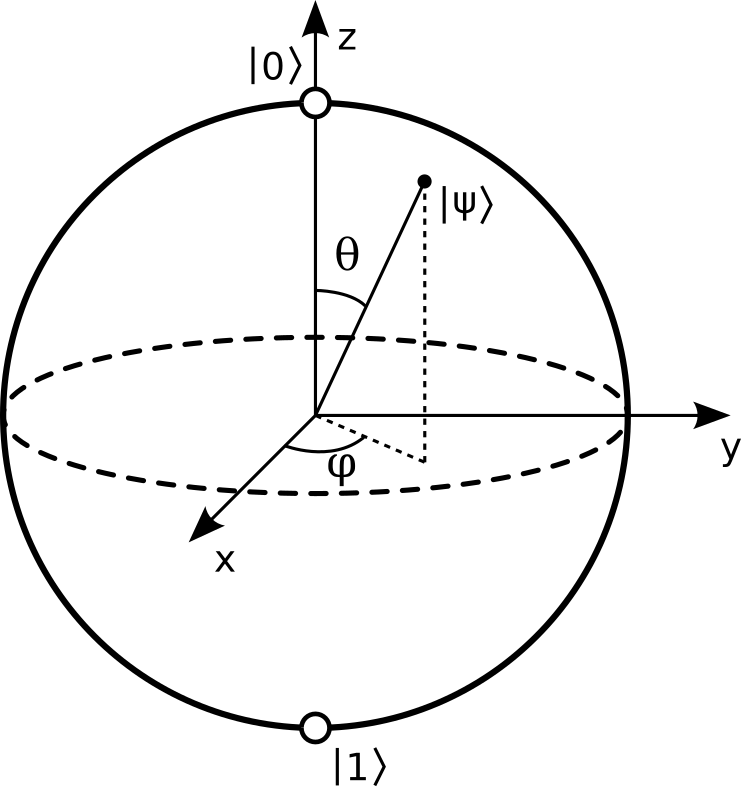
\includegraphics[width=.8\linewidth]{gfx/Bloch_sphere}
    \caption{La sfera di Bloch}
    \label{fig:bloch}
\end{figure}

Gli stati del qubit sull'equatore della sfera, come gli assi coordinati x e y, rappresentano 
sovrapposizioni uniformi dove $\ket{0}$ e $\ket{1}$ hanno entrambi probabilità di misura pari a 
0,5. L'asse x, ad esempio, rappresenta la sovrapposizione uniforme $\frac{1}{\sqrt{2}}
\ket{0} + \frac{1}{\sqrt{2}}\ket{1}$. 
% Come illustrato in Figura, % inserisci riferimento
Qualunque stato bidimensionale arbitrario $\ket{\psi}$ può essere decomposto nei suoi angoli 
polari $\theta$ e $\varphi$ e visualizzato come un vettore sulla sfera di Bloch (dopo essere 
stato normalizzato, se necessario). Tale oggetto è chiamato vettore di Bloch dello stato 
$\ket{\psi}$ del qubit. 

Ad ogni modo, i computer con un solo bit non sono molto utili, e tantomeno i \ac{CQ} con 
un solo qubit. Se prendiamo un byte, ovvero otto bit, possiamo avere una generica 
configurazione 10011101. La rappresentazione associata è 
\begin{equation}
    \ket{1}\otimes\ket{0}\otimes\ket{0}\otimes\ket{1}\otimes\ket{1}\otimes\ket{1}\otimes\ket{0}\otimes\ket{1}.
\end{equation}
Un qubit in questa configurazione appartiene a $\mathbb{C}^2\otimes\mathbb{C}^2\otimes\mathbb{C}^2\otimes\mathbb{C}^2\otimes\mathbb{C}^2\otimes\mathbb{C}^2\otimes\mathbb{C}^2\otimes\mathbb{C}^2 = (\mathbb{C}^2)^{\otimes 8}$. 
Questo spazio vettoriale ha dimensione $2^8=256$. La sua rappresentazione matriciale è allora
\begin{equation}
    \begin{matrix}
        00000000 \\ 
        00000001 \\ 
        \vdots \\ 
        10011101 \\
        \vdots \\
        11111110 \\ 
        11111111
    \end{matrix}
    \begin{pmatrix}
        0 \\ 0 \\ \vdots \\ 1 \\ \vdots \\ 0 \\ 0
    \end{pmatrix}
    .
\end{equation}
La generalizzazione al mondo quantistico è uno stato in sovrapposizione 
\begin{equation}
    \begin{matrix}
        00000000 \\ 
        00000001 \\ 
        \vdots \\
        11111110 \\ 
        11111111
    \end{matrix}
    \begin{pmatrix}
        c_0 \\ c_1 \\ \vdots \\ c_{254} \\ c_{255}
    \end{pmatrix},
\end{equation}
dove $\sum_{i=0}^{255}|c_i|^2=1$. 
Nei computer classici è necessario indicare lo stato di ogni bit in un byte. 
Questo significa scrivere su otto bit. Nel caso quantistico, uno stato di otto 
qubit è dato scrivendo 256 numeri complessi. Questa crescita esponenziale della 
capacità di immagazzinamento dei dati è una delle ragioni per cui i ricercatori 
hanno manifestato interesse per il concetto di quantum computing. 

\subsection{Porte logiche quantistiche} \label{sec:porte_quantistiche}

\begin{definition}
    Una porta logica quantistica è un operatore che agisce sui qubit. Tali operatori 
    saranno rappresentati da matrici unitarie. 
\end{definition}
Le porte logiche quantistiche che agiscono su un sigolo qubit possono essere 
rappresentate come matrici unitarie $2 \times 2$ le cui azioni 
su un qubit possono essere visualizzate come rotazioni o inversioni 
della sfera di Bloch. 

Le porte logiche quantistiche a più qubit agiscono su almeno due qubit 
allo stesso tempo. Similmente alle porte a singolo qubit, una porta quantistica 
a $n$ qubit può essere rappresentata come una matrice unitaria $2^n\times2^n$. 

Tra le porte quantistiche più usate si possono trovare le porte Hadamard, 
NOT, NOT controllata, Toffoli e Fredkin, visibili in figura \ref{fig:porte_1}. 
\begin{figure}[ht!]
    \myfloatalign
    \subfloat[H]{
        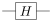
\includegraphics[width=.25\linewidth]{gfx/Hadamard_gate}
    } \quad
    \subfloat[NOT]{
        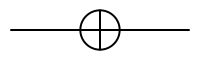
\includegraphics[width=.25\linewidth]{gfx/Qcircuit_NOT}
    } \quad
    \subfloat[cNOT]{
        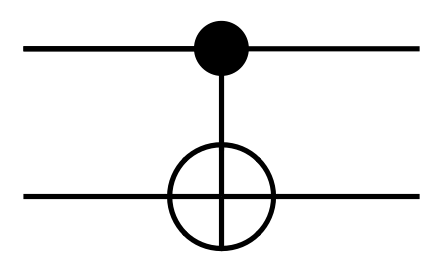
\includegraphics[width=.25\linewidth]{gfx/CNOT_gate}
    } \\ 
    \subfloat[Toffoli]{
        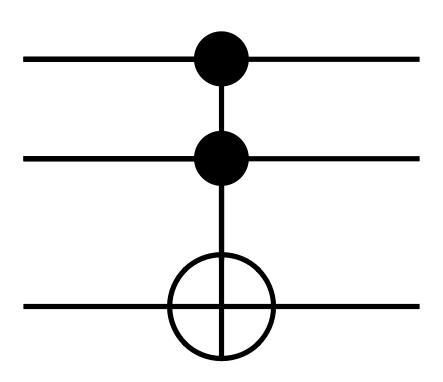
\includegraphics[height=2cm]{gfx/Toffoli_gate}
    } \quad 
    \subfloat[Fredkin]{
        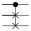
\includegraphics[height=2cm]{gfx/Fredkin_gate}
    }
    
    \caption{Alcune porte quantistiche}
    \label{fig:porte_1}
\end{figure}

Molto importanti sono le tre matrici di Pauli: 
\begin{equation}
    X=\begin{pmatrix}
        0&1\\1&0
    \end{pmatrix},
    \quad Y = \begin{pmatrix}
        0&-1 \\ i&0
    \end{pmatrix},
    \quad Z = \begin{pmatrix}
        1&0 \\ 0&-1
    \end{pmatrix}.
\end{equation}

Altre importanti matrici usate spesso sono 
\begin{equation}
    S=\begin{pmatrix}
        1&0\\0&i
    \end{pmatrix}
    \quad e \quad T = \begin{pmatrix}
        1&0\\0&e^{i\pi/4}
    \end{pmatrix}.
\end{equation}

Le matrici $X$, $Y$ e $Z$ sono modi di girare la 
sfera di Bloch di $\pi$ attorno agli assi $x$, $y$ e $z$ rispettivamente. 
Si noti che $X$ non è altro che la porta NOT, e trasforma $\ket{0}$ in $\ket{1}$ 
e viceversa. Ma per di più porta tutto quello che si trova sopra l'equatore 
sotto di esso. Le altre matrici di Pauli funzionano in maniera simile. 

In alcuni casi non si vuole effettuare una rotazione completa di $\pi$ 
ma si vuole ruotare la sfera di un angolo $\theta$ lungo una particolare direzione. 
In questo caso, dato un vettore tridimensionale $D=(D_x, D_y, D_z)$ di modulo 1, 
possiamo costruire una rotazione della sfera di Bloch attorno ad esso in questo 
modo: 
\begin{equation}
    R_D(\theta)=\cos\frac{\theta}{2}\mathbb{1} - i \sin \frac{\theta}{2} 
    (D_x X + D_y Y + D_z Z). 
\end{equation}

La sfera di Bloch è utile solo per visualizzare stati e trasformazioni di un qubit. 
Quando abbiamo a che fare con più qubit, la dimensionalità degli stati non ci 
permette di avere una rappresentazione intuitivamente semplice. 

Tra le porte a più qubit che verranno usate in questa tesi ci sono le porte controllate: 
queste hanno il loro effetto se tutti i qubit di controllo sono nello stato $\ket{1}$, 
altrimenti lasciano i bersagli della loro azione immutati. 
Si propone a titolo esemplificativo la porta Deutsch, ovvero una rotazione di fase applicata 
a un qubit bersaglio, condizionata dallo stato di due qubit di controllo: 
\begin{equation}
    D_{\theta} : \ket{a,b,c} \mapsto \begin{cases}
        i \cos(\theta)\ket{a,b,c} + \sin(\theta)\ket{a,b,1-c} \quad &\text{per}\, a=b=1, \\ 
        \ket{a,b,c} \quad &\text{altrimenti}.
    \end{cases}
\end{equation}
Nei capitoli successivi verrà implementata la porta $C^n R_y (\theta)$, che effettua una 
rotazione di angolo $\theta$ attorno all'asse y, con $n$ qubit di controllo. 

% *************************************************
% Non si è detto cosa sia un insieme universale di porte
% *************************************************

Le due porte appena descritte non si trovano generalmente nel set universale di porte 
del computer quantistico che si va ad utilizzare, ma devono 
essere approssimate attraverso una successione di porte di base, che può essere più o 
meno lunga. La ricerca di nuovi modi per implementare porte complesse in maniera 
nativa \cite{PhysRevApplied.9.051001} è uno degli sforzi per contrastare il fenomeno della 
decoerenza, uno degli ostacoli sostanziali nel calcolo quantistico. 

\subsection{Decoerenza} \label{sec:decoerenza}

\begin{definition}
    La decoerenza è la perdita di purezza dello stato di un sistema quantistico come risultato 
    di interazione con l'ambiente. 
\end{definition}

Esistono due paramentri per descrivere quanto è stabile un sistema nei confronti della decoerenza \cite{IBM_decoherence}: 
\begin{itemize}
    \item il tempo di decoerenza longitudinale, legato all'emissione energetica, 
    ovvero il decadimento degli stati più energetici verso quelli meno energetici
    (si pensi ad un elettrone nello stato eccitato che decade verso lo stato fondamentale in un atomo);
    \item il tempo di decoerenza trasversale, legato al defasamento, tempo in cui 
    statisticamente uno stato di sovrapposizione decade in una configurazione ben definita. 
\end{itemize}


\section{Machine learning classico} \label{sec:machine_learning}

% ***************************************
% Introduzione al machine learning
% ***************************************

\begin{definition}
    Il machine learning, una branca dell'\ac{IA}, è l'applicazione e lo studio  
    di algoritmi che danno un significato ai dati. 
\end{definition}

Si può dividere la materia in tre tipi principali: l'apprendimento supervisionato, 
l'apprendimento non supervisionato e l'apprendimento per rinforzo. 
Qui si parlerà solo di apprendimento supervisionato. 

L'obiettivo dell'apprendimento supervisionato è di imparare un modello da dati 
etichettati che ci permetta di fare previsioni su dati futuri sconosciuti. 
Con il termine supervisionato si intende l'esistenza di un insieme di campioni 
dove i risultati aspettati (l'appartenenza ad una determinata classe, il 
risultato di una funzione) sono già conosciuti. 

La classificazione
\marginpar{Un esempio di classificatore supervisionato è il filtro contro la posta 
indesiderata, che si può addestrare con un insieme di email già classificate come 
spam o non spam, in modo che esso riconosca in quale categoria vanno le nuove email 
in arrivo.}
è una sottocategoria del machine learning supervisionato il cui 
scopo è di predire le etichette di classe che categorizzano delle nuove istanze, 
basandosi su osservazioni passate. Tali classi sono valori discreti non ordinati 
che possono rappresentare l'appartenenza ad un gruppo delle istanze. 

\subsection{KNN} \label{sec:knn}

Il \acf{KNN} è un algoritmo di machine learning supervisionato per la classificazione. 
È chiamato lazy learner, in quanto non apprende una regola su come discriminare 
le classi dei vettori, ma memorizza il data set di apprendimento tutto intero. 
L'algoritmo in sé è piuttosto semplice e può essere riassunto nei seguenti passaggi: 
\begin{itemize}
    \item scegli il numero $k$ e una metrica per la distanza; 
    \item trova i $k$ elementi più vicini al campione da classificare; 
    \item assegna l'etichetta di classe con un voto a maggioranza. 
\end{itemize}

\begin{figure}[h!]
    \centering
    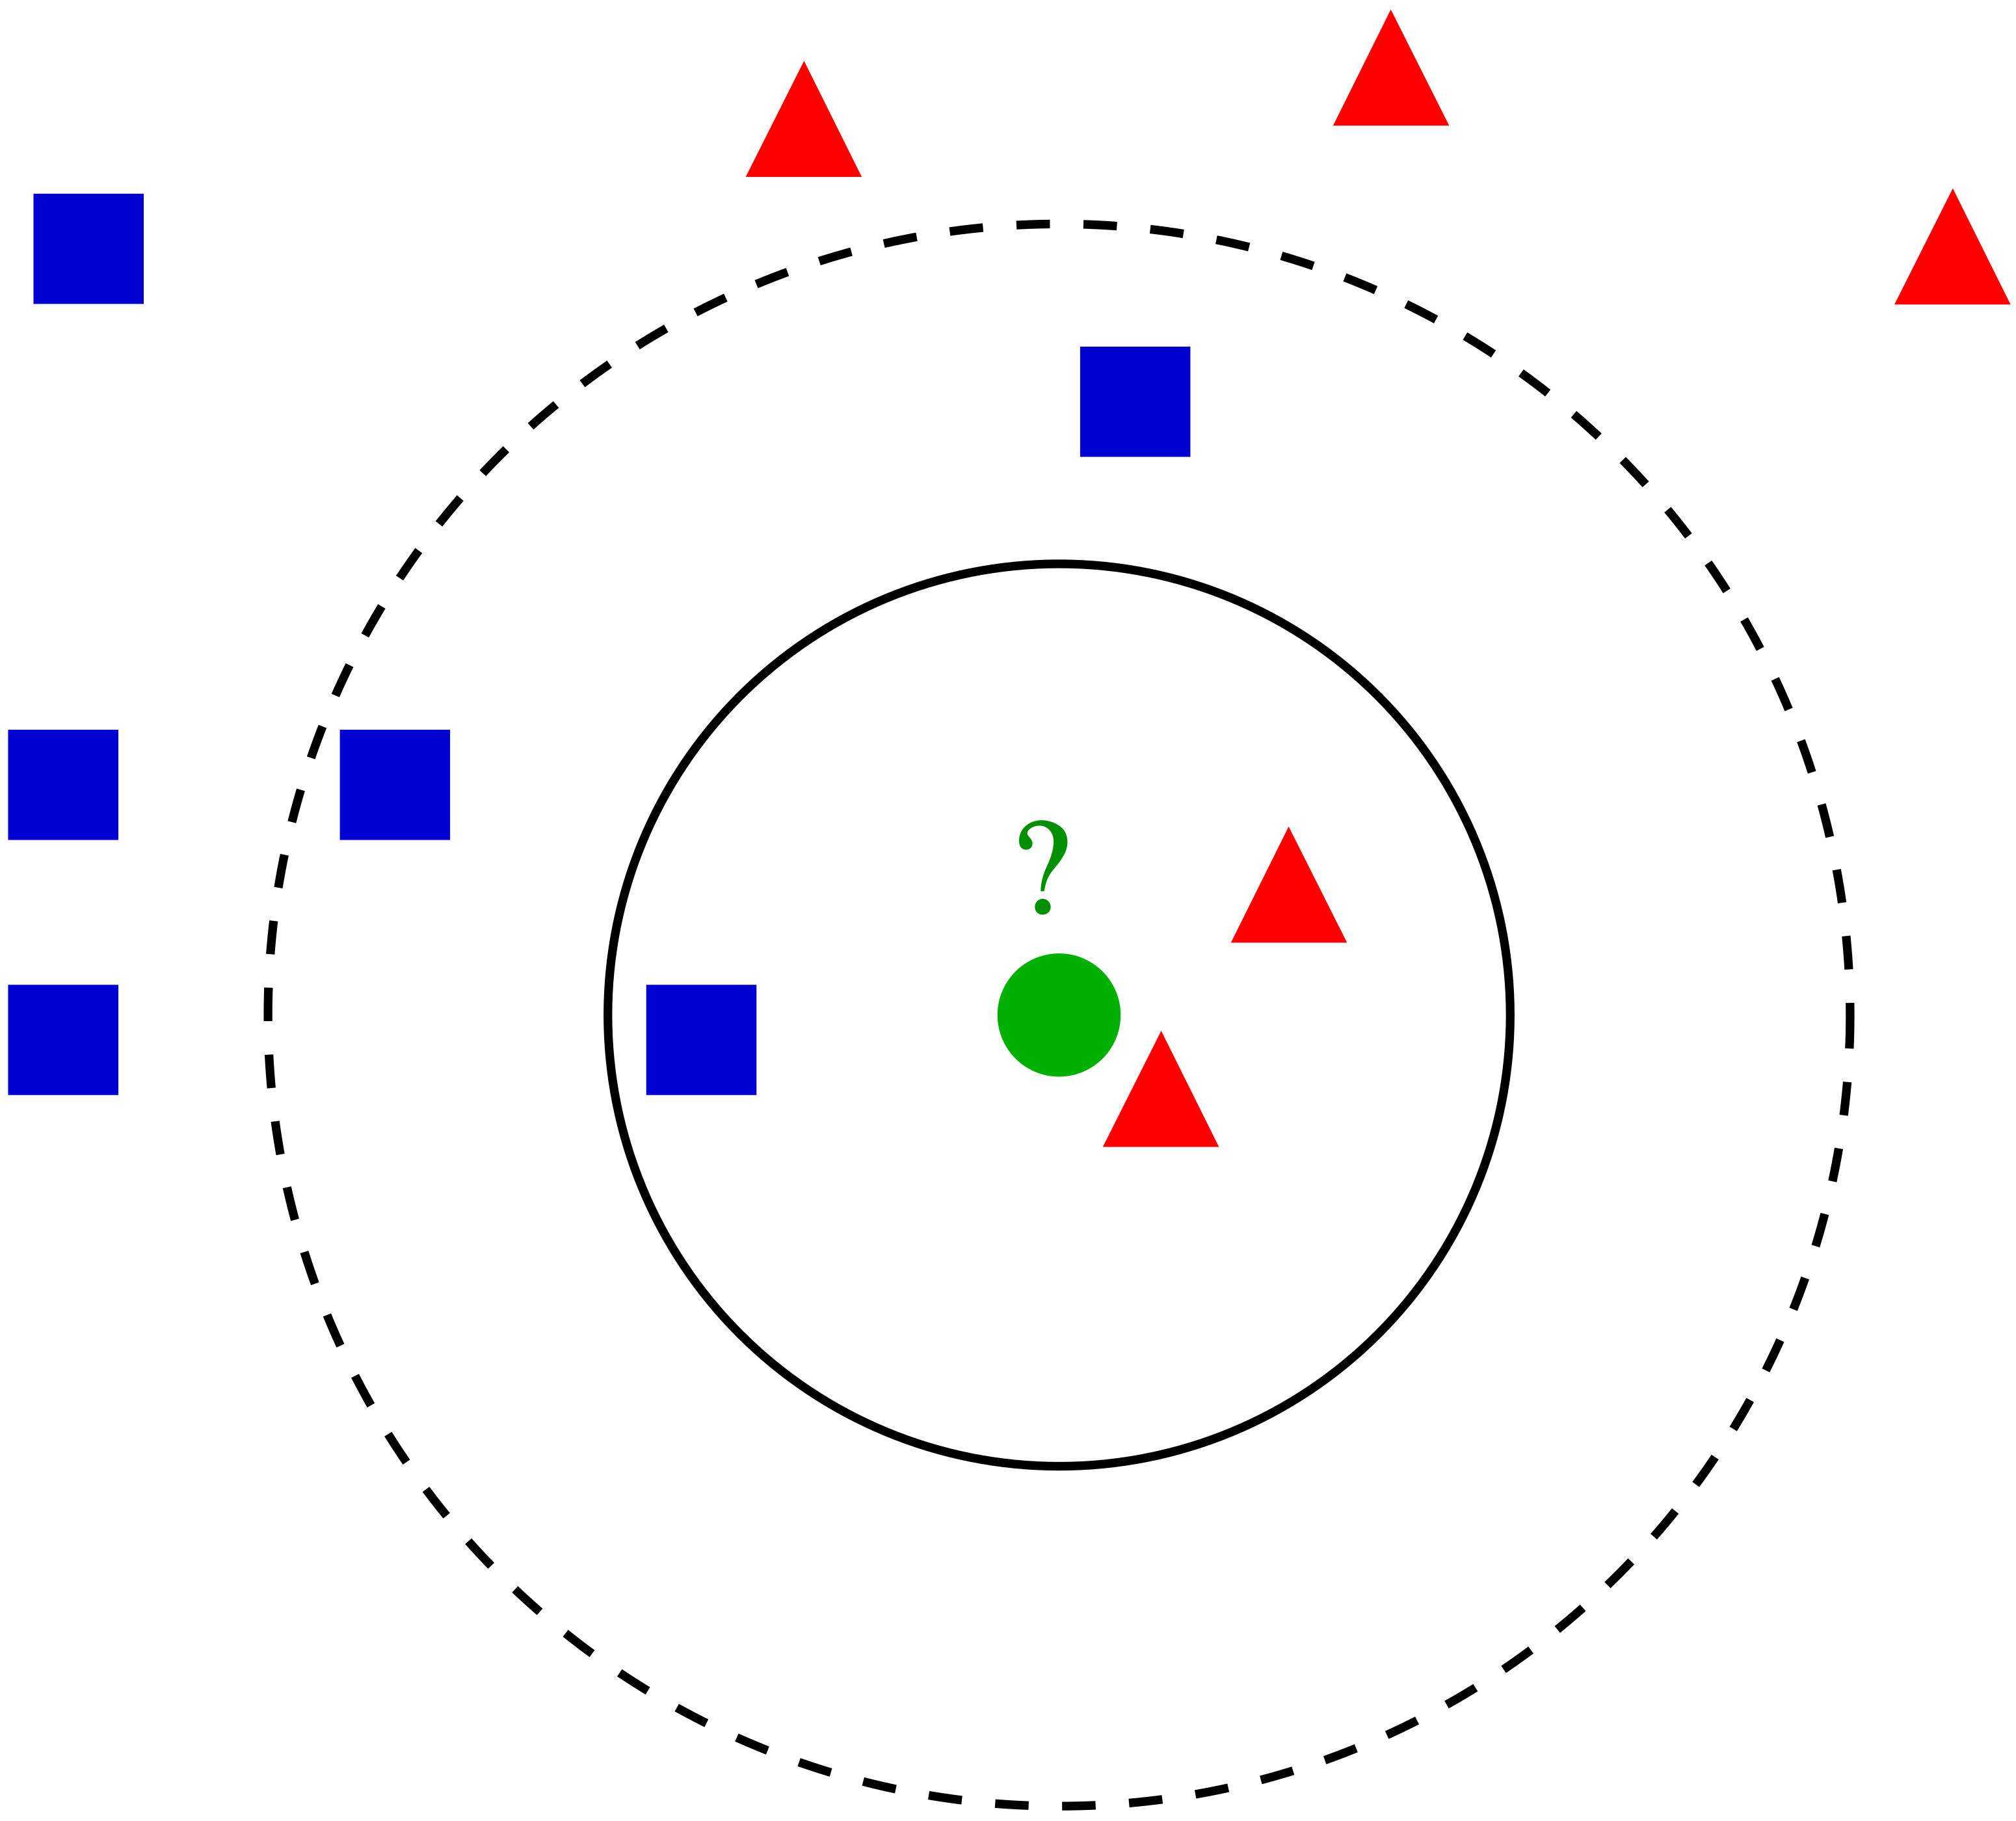
\includegraphics[width=.8\linewidth]{gfx/KnnClassification}
    \caption{Rappresentazione dell'algoritmo \ac{KNN}}
    \label{fig:knn}
\end{figure}

In base alla metrica scelta, l'algoritmo \ac{KNN} trova i $k$ campioni 
nel data set di apprendimento che sono più vicini (simili) al punto 
da classificare. La classe del nuovo punto è allora determinata da un 
voto a maggioranza basato sulla classe a cui appartengono i suoi $k$ 
vicini (vedi figura \ref{fig:knn}). 

Il vantaggio principale di 
questo approccio basato sulla memoria è che il classificatore si 
adatta immediatamente man mano che aggiungiamo vettori di apprendimento. 
Dall'altro lato, il difetto è che la complessità computazionale per 
classificare nuovi campioni cresce al più linearmente con il numero di 
vettori di apprendimento. Per di più, non possiamo ignorare a priori 
alcun vettore di training dato che non c'è un vero e proprio apprendimento. 
Così, lo spazio di archiviazione e il numero di distanze da calcolare possono 
diventare un problema nodale quando si lavora con grandi data set. \cite{pml}

\section{Machine learning quantistico} \label{sec:qml}

% ***************************************
% Introduzione al quantum machine learning, vedi articolo di Biamonte e Lloyd
% ***************************************

% Quantum mechanics is well known to produce atypical patterns in data. Classical machine learning methods such as deep neural networks frequently have the feature that they can both recognize statistical patterns in data and produce data that possess the same statistical patterns: they recognize the patterns that they produce. This observation suggests the following hope. If small quantum information processors can produce statistical patterns that are computationally difficult for a classical computer to produce, then perhaps they can also recognize patterns that are equally difficult to recognize classically.

Il machine learning quantistico è la materia che unisce machine learning e 
meccanica quantistica. Bimonte et al. \cite{Biamonte2017} scrivono: 
% For example, quantum computers can search an unsorted database with N entries in time proportional to √N—that is, O(√N)—where a classical computer given blackbox access to the same database takes time proportional to N: thus the quantum computer exhibits a square-root speedup over the classical computer. Similarly, quantum computers can perform Fourier transforms over N data points, invert sparse N × N matrices, and find their eigenvalues and eigenvectors in time proportional to a polynomial in log2N, where the best known algorithms for classical computers take time proportional to Nlog2N: thus the quantum computer exhibits an exponential speedup over the best classical computer algorithms.
\begin{quote}
    la meccanica quantistica segue notoriamente modelli atipici. 
    I metodi di machine learning classico come le reti neurali profonde 
    (deep neural network) frequentemente hanno la caratteristica di poter sia 
    riconoscere modelli statistici sia produrre dati che ne possiedano gli 
    stessi andamenti: riconoscono i motivi che producono. Questa osservazione 
    porta alla seguente speranza. Se piccoli processori di informazioni 
    quantistiche possono produrre motivi statistici che sono computazionalmente 
    difficili da produrre per un computer classico, allora forse essi possono 
    anche riconoscere motivi che sono ugualmente difficili da riconoscere 
    classicamente. 
    \marginpar{
    Per esempio, i computer quantistici possono cercare in una banca dati non ordinata con 
    $N$ voci in un tempo proporzionale a $\sqrt{N}$, ovvero $\mathcal{O}(\sqrt{N})$, mentre 
    un computer classico con accesso a scatola nera alla stessa banca dati impiega un tempo 
    proporzionale ad $N$: dunque il computer quantistico esibisce un'accelerazione 
    che va come la radice quadrata rispetto al computer classico. 
    }
    La realizzazione di questa speranza dipende dal fatto che si possano trovare algoritmi 
    quantistici efficienti per il machine learning. Un algoritmo quantistico è un insieme di 
    istruzioni che risolvono un problema, come determinare se due grafici sono isomorfi, 
    che possono essere eseguite su un computer quantistico. Il software del quantum machine 
    learning fa uso degli algoritmi quantistici come parte di un'implementazione maggiore. 
    Analizzando i passi prescritti dagli algoritmi quantistici, diventa chiaro che hanno il 
    potenziale di superare in prestazioni gli algoritmi classici per problemi specifici (cioè, 
    ridurre il numero di passi necessari). Questo potenziale è conosciuto come accelerazione 
    quantistica \cite{Ronnow420}. 
\end{quote}
% The realization of this hope depends on whether efficient quantum algorithms can be found for machine learning. A quantum algorithm is a set of instructions solving a problem, such as determining whether two graphs are isomorphic, that can be performed on a quantum computer. Quantum machine learning software makes use of quantum algorithms as part of a larger implementation. By analysing the steps that quantum algorithms prescribe, it becomes clear that they have the potential to outperform classical algorithms for specific problems (that is, reduce the number of steps required). This potential is known as quantum speedup.

Nel quantum machine learning il computer quantistico analizza dati classici, che sono 
codificati come stati quantistici, oppure dati quantistici. Sempre afferente allo stesso 
campo è l'uso di tecniche di machine learning classico per trovare modelli in dinamica 
quantistica. Ci si limiterà al caso dell'uso di computer quantistici per analizzare dati 
classici. 

Nella sezione seguente si descriverà la versione quantistica dell'algoritmo \ac{KNN} visto 
nella sezione \ref{sec:knn}, proposta ed implementata sul processore quantistico a 5 
qubit dell'IBM da Schuld et al. \cite{10.1007/978-3-319-13560-1_17}, \cite{schuld}. 

\subsection{QKNN} \label{sec:qknn}

% ****************************************************
% Desrizione dell'algoritmo di Schuld
% ****************************************************

L'idea alla base dell'algoritmo \ac{QKNN} è di usare il fenomeno di interferenza 
quantistica per ottenere una misura della distanza con un calcolo in parallelo. 
Dotandosi di una procedura efficiente per la preparazione dello stato, l'algoritmo 
ottiene la riduzione logaritmica nelle dimensioni e nel numero di dati in input che 
ci si aspetta usando una codifica quantistica dei dati 
classici \cite{quantum_support_vector_machine}.
Si considera l'attività di classificazione supervisionata di un motivo binario: 
dato un data set $D=\{ (t^1,c^1),\ldots,(t^M,c^M) \}$ di input $t^m\in\mathbb{R}^N$ 
con le rispettive etichette di classe $c^m\in \left\{ -1,1 \right\} $ per $m=1,\ldots,M$ 
e un nuovo input $x\in\mathbb{R}^N$, si trovi l'etichetta $c\in\left\{ -1,1 \right\}$ che 
corrisponde al nuovo input. 

Il classificatore, implementato tramite un circuito di interferenza quantistica 
ed una funzione di soglia, è dato da 
\begin{equation}
    c = \text{sgn} \left( \sum_{m=1}^M c^m \left[ 1 - \frac{1}{4M} | x - t^m |^2 \right] \right). 
\end{equation}
L'algoritmo che implementa il classificatore codifica le caratteristiche dell'input nelle 
ampiezze di probabilità del sistema quantistico e le manipola attraverso porte 
quantistiche; questa strategia è uno dei fattori ritenuti responsabili 
dell'accelerazione quantistica. 
Dato un vettore $x\in\mathbb{R}^N$ normalizzato con modulo unitario e $N=2^n$, 
la codifica nelle ampiezze permette di descrivere lo stato con un registro di $n$ qubit 
$\ket{\psi_x} = \sum_{i=0}^{N-1} x_i \ket{i}$, dove $\ket{i}$ è un registro indice che 
segnala l'$i$-esima componente del vettore classico attraverso l'$i$-esimo elemento della 
base computazionale. 

% La parte sotto è un po' contorta

% L'obiettivo è di classificare una registro di qubit in entrata basandosi 
% su un numero più o meno grande di configurazioni di qubit di apprendimento. 
% Ogni configurazione di apprendimento appartiene ad una certa classe, che è 
% codificata in un registro quantistico di classe in entanglement con la rispettiva 
% configurazione di apprendimento. L'idea principale è che l'algoritmo \ac{KNN} 
% calcola la distanza tra il motivo in entrata ed ogni configurazione di 
% apprendimento attraverso una serie di porte quantistiche. 
% Successivamente, queste distanze sono invertite in modo che i vettori di 
% apprendimento vicini a quello di input hanno l'inverso della distanza 
% maggiore rispetto ai vettori di apprendimento più remoti. Queste distanze inverse 
% sono poi scritte nelle corrispondenti ampiezze dello stato di classe. 
% Si noti che il modulo quadro di un'ampiezza di un particolare stato di classe 
% determina la probabilità di misurare quella classe. 
% Quindi, la probabilità di misurare una data classe dipende adesso dall'inverso 
% delle distanze tra i vettori di apprendimento della classe in esame ed il 
% vettore d'input. L'inverso della distanza può essere visto come un peso 
% dipendente dalla distanza, dato che aumenta la probabilità di misurare la 
% classe con i vettori di apprendimento più vicini a quello d'input. 
% I passaggi necessari per l'implementazione dell'algoritmo \ac{KNN} quantistico 
% sono evidenziati in dettaglio qui di seguito. 

Il primo passo dell'algoritmo consiste nel preparare una 
\emph{sovrapposizione dell'insieme di apprendimento} che 
ne contenga i dati codificati. 
Usando un idoneo schema di preparazione dello stato (nella sezione \ref{sec:ff-qram} 
se ne vedrà un esempio pratico), 
il circuito di classificazione porta un sistema di $n$ 
qubit nello stato 
\begin{equation}
    \ket{D} = \frac{1}{\sqrt{2MC}} \sum_{m=1}^M \ket{m} 
    \left( \ket{0}\ket{\psi_x} + \ket{1}\ket{\psi_{t^m}} \right)
    \ket{c^m}.
\end{equation}
Qui $\ket{m}$ è un registro indice che prende valori 
$m=1,\ldots,M$ e che contrassegna l'$m$-esimo vettore 
di apprendimento. 
Il secondo registro è un singolo qubit ancilla, il cui 
stato eccitato è in entanglement con il terzo registro 
che codifica l'$m$-esimo stato di apprendimento 
$\ket{\psi_{t^m}} = \sum_{i=0}^{N-1} t_i^m \ket{i}$, 
mentre il suo stato fondamentale è in entanglement con 
il terzo registro che codifica il vettore d'input 
$\ket{\psi_x} = \sum_{i=0}^{N-1} x_i \ket{i}$. 
Il quarto registro codifica la classe nell'ampiezza dei propri qubit. 
Effettivamente, si crea una funzione d'onda che contiene 
i vettori di apprendimento insieme ad $M$ copie del nuovo 
input. La costante di normalizzazione $C$ dipende dal 
processo di ottimizzazione dei dati; 
assumeremo in seguito che i vettori di apprendimento siano 
normalizzati e quindi $C=1$. 

Dopo aver preparato lo stato iniziale, il circuito quantistico 
consiste di sole tre operazioni. Prima, l'applicazione di 
una porta Hadamard sull'ancilla fa interferire le copie 
del vettore d'input con i vettori di apprendimento: 
\begin{equation}
    \frac{1}{2\sqrt{M}} \sum_{m=1}^M \ket{m}
    \left( \ket{0}\ket{\psi_{x+t^m}} + \ket{1}  
    \ket{\psi_{x-t^m}} \right) \ket{c^m},
\end{equation}
dove $\ket{\psi_{x \pm t^m}} = \ket{\psi_x} \pm \ket{\psi_{t^m}}$. 

La seconda operazione è una misura condizionale che seleziona 
il ramo con l'ancilla nello stato $\ket{0}$. Questa 
postselezione ha successo con probabilità 
$p_\text{acc} = \frac{1}{4M}\sum_m |x+t^m|^2$. 
È più probabile che abbia successo se la distanza euclidea 
al quadrato complessiva dell'insieme dati di apprendimento 
rispetto al nuovo input è piccola. 
% Mostreremo... ***************
Se la misura condizionale ha successo, lo stato risultanta 
è dato da 
\begin{equation}
    \frac{1}{2\sqrt{Mp_{\text{acc}}}} \sum_{m=1}^M \sum_{i=1}^N 
    \ket{m} ( x_i + t_i^m ) \ket{i} \ket{c^m}.
\end{equation}
Le ampiezze pesano i qubit classe $\ket{c^m}$ con la 
distanza dell'$m$-esimo vettore dati dal nuovo input. 
In questo stato, la probabilità di misurare il qubit 
classe nello stato $\ket{s}$ 
\begin{equation} \label{eq:prob.classe}
    p(\ket{c}=\ket{s}) = \frac{1}{4Mp_{\text{acc}}} 
    \sum_{m|\ket{c}=\ket{s}} |x+t^m|^2,
\end{equation}
riflette la probabilità di predire la classe $s$ per il 
nuovo input. 

La scelta di vettori caratteristica normalizzati assicura che \\ 
$\frac{1}{4Mp_{\text{acc}}}\sum_m |x+t^m|^2 = 
1 - \frac{1}{4Mp_{\text{acc}}}\sum_m |x-t^m|^2$, e la scelta 
della classe con maggior probabilità in questo modo 
implementa il classificatore. 
Questo significa che se il vettore d'input è molto 
vicino ai vettori di training di una data classe, 
quella classe uscirà come risultato più frequentemente 
delle altre. 

% Il \acf{ML}, una sottodisciplina dell'intelligenza artificiale, prova a dare la 
% capacità ai computer di imparare dai dati senza che un umano programmi 
% esplicitamente le sue azioni. Può essere suddiviso nei tre maggiori campi di 
% supervisionato, non supervisionato e apprendimento per rinforzo (Schuld, 
% Sinaskiy, Petruccione, 2015). Solo il machine learning supervisionato sarà 
% introdotto poiché questa tesi di ricerca si focalizza esclusivamente su 
% algoritmi di machine learning supervisionato. 

% L'idea principale del machine learning supervisionato è di addestrare un 
% algoritmo su un insieme di dati \emph{etichettati} contenente, per esempio, 
% immagini di frutti con i corrispondenti nomi cosicché possa essere usato per 
% etichettare nuove immagini che non fanno parte dell'insieme dati di addestramento. 
% Dato che i campioni nell'insieme dati di addestramento sono etichettati, 
% il processo è detto essere supervisionato. 

% Più formalmente, nel machine learning supervisionato si è di fronte a paia di 
% variabili di input (x) e di output (o) e si suppone che l'algoritmo di machine 
% learning impari la funzione $f$ che mappa gli input sui relativi output: 
% \begin{equation} \label{eq:2.38}
%     f(x) = o.
% \end{equation}
% Così, l'algoritmo dovrebbe approssimare la funzione di mappatura $f$ a tal punto 
% che può predire l'output $o$ per nuovi dati di input sconosciuti $\tilde{x}$ 
% (C. M. Bishop, 2006). La seguente sezione introdurrà un algoritmo ben noto nel 
% campo del \ac{ML} supervisionato: l'algoritmo k-nearest neighbours classico. 















% Si immagini di lavorare per una compagnia che gestisce un motore di ricerca e 
% e che venga assegnato il compito di classificare immagini ignote di frutti come 
% mele o banane. Per addestrare l'algoritmo di classificazione, vengono fornite 
% cinque differenti immagini di mele e cinque differenti immagini di banane. 
% Questo verrà chiamato l'\emph{insieme dati di apprendimento} (training data set) 
% $D_T$. Le immagini in $D_T$ potrebbero essere prese da angolazioni diverse, in 
% condizioni di luce varie ed includere mele e banane di colori diversi. 

% La maggior parte delle volte, usare la rappresentazione completa dei pixel di 
% ogni immagine per la classificazione non porta a risultati ottimali. Dunque, il 
% passo successivo è di selezionare un certo numero di caratteristiche (features) 
% estratte dalle immagini nell'insime di apprendimento che possono essere usate per 
% differenziare le mele dalle banane. Tali caratteristiche possono essere il codice 
% del colore più frequente tra i pixel, dato che mele e banane hanno spettri di 
% colore diversi. Usare una misura della curvatura dell'oggetto principale 
% nell'immagine è un'altra possibilità, dato che una mela è quasi sferica mentre 
% una banana assomiglia più ad una linea curva. 

% Selezionando ed estraendo caratteristiche, la dimensionalità dell'insieme dati 
% di apprendimento è drasticamente ridotta da qualche migliaio di pixel ad una 
% manciata di caratteristiche. Le $m$ caratteristiche estratte dalla $j$-esima 
% immagine sono conservate nel $vettore caratteristica$ $m$-dimensionale 
% $\vec{v}_j$. Matematicamente, l'insieme dati di apprendimento $D_T$ consiste di 
% dieci vettori caratteristica $\vec{v}_0, \vec{v}_1, \ldots, \vec{v}_9$, ognuno 
% assegnato alla classe $A$ (mela) o alla classe $B$ (banana). I vettori di 
% apprendimento sono visualizzati come cerchi chiari e scuri in figura. 

% % Metti figura ****************************

% Data una nuova immagine di una mela o una banana, prima si estraggono le stesse 
% $m$ caratteristiche da essa e si conservano nel vettore d'input $\vec{x}$. Dei 
% tanti algoritmi, si sceglie di usare l'algoritmo \ac{KNN}, dato che è un 
% classificatore non parametrico, cioè non fa assunzioni pregresse sulla classe 
% della nuova immagine. Dato un nuovo vettore d'input $\vec{x}$ non classificato 
% (stella nella figura), % inserisci riferimento a figura
% l'algoritmo considera i $k$ elementi più vicini tra quelli dell'insieme dati 
% di apprendimento (usando una misura di distanza predefinita) e classifica 
% $\vec{x}$, basandosi su un voto a maggioranza, come $A$ o $B$. Così, $k$ è un 
% numero intero positivo, solitamente scelto piccolo ed il suo valore determina 
% il risultato della classificazione. Praticamente, nel caso $k=3$ in figura, 
% % aggiungi riferimento a figura ***************
% il vettore $\vec{x}$ sarà classificato come appartenente alla classe $B$ (scuro) 
% ma nel caso $k=6$ sarà etichettato nella classe $A$ (chiaro). 

% % figura classe a classe b ******************

% Nel caso $k=10$, $\vec{x}$ sarà semplicemente assegnato alla classe con più 
% membri. In questo caso, ai vettori di addestramento dovrebbe assegnarsi dei pesi 
% dipendenti dalla distanza (come $\frac{1}{\text{distanza}}$) per aumentare 
% l'influenza dei vettori più vicini al vettore d'input rispetto a quelli più 
% lontani. 











% \subsection{Complessità algoritmica: notazione O-grande}

% Nei campi dell'informatica e della quantum information, la cosiddetta 
% \emph{notazione O-grande}, inizialmente descritta da Bachmann (1894), 
% % inserisci fonte *****************************
% è spesso usata per descrivere come l'esecuzione di un algoritmo dipende 
% da variabili come l'accuratezza desiderata, il numero di vettori d'input o la 
% loro dimensione. Per questo, essa è un modo di quantificare la \emph{complessità 
% in termini di tempo dell'algoritmo} di un algoritmo quantistico. Nelle sezioni 
% successive di questa tesi, la notazione O-grande sarà usata come uno strumento 
% per quantificare possibili accelerazioni quantistiche negli algoritmi \ac{KNN} di 
% machine learning quantistico. 

% % scatola definizione di big-O **************

% % continuare ********************




% Un buon esempio di un'implementazione fisica di un qubit è il singolo elettrone di un atomo di 
% idrogeno abbozzato in figura. % metti riferimento a figura
% Solitamente l'elettrone si trova % è trovato
% nel suo stato fondamentale, che può essere definito come lo stato $\ket{0}$ del qubit. 
% Usando un impulso laser, l'elettrone può essere eccitato verso il guscio di valenza successivo più 
% energetico, che può essere definito come lo stato $\ket{1}$  del qubit. Dopo del tempo $t$ 
% l'elettrone decadrà per decoerenza verso il suo stato fondamentale $\ket{0}$; questo tempo è 
% chiamato \emph{tempo di decoerenza longitudinale} o \emph{di smorzamento dell'ampiezza} ed è 
% un parametro importante per misurare la vita dei qubit. % Fonte Chuang, 2003

% Figura ***********************************

% Un bit classico non probabilistico può assumere solo uno dei suoi due possibili valori alla volta. 
% Qui si potrebbe mettere una nota sui bit probabilistici
% Al contrario, i qubit obbediscono alle leggi della meccanica quantistica, il che dà luogo 
% all'importante proprietà che, oltre ad essere in un definito stato $\ket{0}$ o $\ket{1}$, 
% possono anche essere in una sovrapposizione di due stati. Matematicamente ciò è espresso 
% attraverso la combinazione lineare degli stati $\ket{0}$ e $\ket{1}$
% \begin{equation} \label{eq:2.1}
%     \ket{\psi} = \alpha \ket{0} + \beta \ket{1}, \quad \alpha, \beta \in \mathbb{C},
% \end{equation}
% dove $\alpha$ e $\beta$ sono coefficienti complessi e ci si riferisce spesso a loro come ampiezze. 
% Qualsiasi ampiezza $\eta$ può essere ulteriormente suddivisa in un fattore di fase complesso 
% $e^{i\varphi}$ ed un numero reale non negativo $\xi$ cosicché
% \begin{equation}
%     \eta = e^{i\varphi} \xi.
% \end{equation}
% Nella prima equazione, $\ket{0}$ è la rappresentazione nella notazione di Dirac del fatto che il 
% qubit sia nello stato 0 e può essere rappresentato come un elemento di uno spazio vettoriale 
% complesso bidimensionale $H_2$, % metti il font giusto ad H
% detto spazio di Hilbert. Inizialmente definito da Dirac, % metti fonte 1939
% l'oggetto 
% \begin{equation}
%     \ket{\varphi},
% \end{equation}
% è chiamato \emph{ket} e il suo coniugato hermitiano 
% \begin{equation}
%     \ket{\varphi}^\dagger = \bra{\varphi}
% \end{equation}
% è chiamato \emph{bra}. Il coniugato hermitiano, denotato con una daga ($\dagger$), di p.e. un 
% vettore colonna $c$ bidimensionale a valori complessi $c_1$ e $c_2$, 
% \begin{equation}
%     c = 
%     \begin{pmatrix}
%         c_1\\c_2
%     \end{pmatrix},
% \end{equation}
% è ottenuto prendendo il complesso coniugato di ciascun valore e trasponendo il vettore risultante: 
% \begin{equation}
%     c^\dagger = 
%     \begin{pmatrix}
%         c_1\\c_2
%     \end{pmatrix}^\dagger
%     = 
%     \begin{pmatrix}
%         c_1^* & c_2^*
%     \end{pmatrix},
% \end{equation}
% dove i complessi coniugati sono indicati con un asterisco in apice ($*$).
% Il coniugato hermitiano è definito sia per vettori che per matrici quadrate. 
% Il prodotto interno tra un bra e un ket è chiamato \emph{bra-ket} ed è scritto 
% \begin{equation}
%     \braket{\varphi|\varphi}.
% \end{equation}
% Si noti che tutte le sezioni seguenti faranno uso intensivo della notazione bra-ket. 
% Gli stati quantistici $\ket{0}$ e $\ket{1}$ sono chiamati la base computazionale e 
% costituiscono una base ortonormale di $H_2$. Quando un qubit è espresso in termini 
% dei due stati $\ket{0}$ e $\ket{1}$, si dice che sia nella sua \emph{base normale}. 
% Per motivi di chiarezza, $\ket{0}$ e $\ket{1}$ possono essere rappresentati con i vettori 
% bidimensionali 
% \begin{equation} \label{eq:2.8}
%     \ket{0} \cong \begin{pmatrix}
%         1\\0
%     \end{pmatrix}
%     \text{e} \ket{1} \cong \begin{pmatrix}
%         0\\1
%     \end{pmatrix}.
% \end{equation}
% Si noti che un ket e la sua rappresentazione vettoriale non sono lo stesso oggetto, 
% dato che, per essere ben definito, un vettore ha bisogno della specificazione di una base, 
% laddove un ket non lo richiede. Questa tesi farà uso del simbolo $\cong$ quando si cambia tra 
% i due diversi modi di rappresentare un ket. Sostituendo i vettori dell'Eq. \ref{eq:2.8} 
% nell'Eq. \ref{eq:2.1} si ottiene la rappresentazione vettoriale di $\ket{\psi}$
% \begin{equation} \label{eq:2.9}
%     \psi \cong \alpha \begin{pmatrix}
%         1\\0
%     \end{pmatrix} + \beta \begin{pmatrix}
%         0\\1
%     \end{pmatrix} = \begin{pmatrix}
%         \alpha \\ \beta
%     \end{pmatrix}.
% \end{equation}

% Sebbene un qubit possa essere in una sovrapposizione di stati $\ket{0}$ e $\ket{1}$, quando 
% misurato assumerà un valore preciso tra $\ket{0}$, con probabilità 
% \begin{equation}
%     P(\ket{0}) = |\alpha|^2,
% \end{equation}
% e $\ket{1}$, con probabilità 
% \begin{equation}
%     P(\ket{1}) = |\beta|^2.
% \end{equation}
% Il fatto che la probabilità di misurare un particolare stato è uguale al quadrato del modulo 
% della rispettiva ampiezza fu postulato per la prima volta da Born % Fonte 1954
% e, dunque, è chiamata regola di Born. Visto che la probabilità totale di misurare un qualunque 
% valore deve essere unitaria, deve soddisfarsi la condizione di normalizzazione 
% \begin{equation}
%     |\alpha|^2 + |\beta|^2 = 1.
% \end{equation}

% Se prendiamo uno stato in cui si ha, per esempio, $\alpha = \frac{1}{\sqrt{2}}$ e 
% $\beta = \frac{i}{\sqrt{2}}$, abbiamo che il qubit è in una sovrapposizione quantistica, 
% cosa impossibile da ottenere con un computer classico. Legato a questa caratteristica 
% c'è un altro importante parametro della vita di un qubit: il \emph{tempo di coerenza 
% trasversale} o \emph{di smorzamento della fase}. 
% Esso è misurato preparando la sovrapposizione uniforme $\frac{\ket{0} + \ket{1}}{\sqrt{2}}$: 
% per via dell'inevitabile interazione con l'ambiente, dopo del tempo $t$ il comportamento 
% quantistico sarà perso e lo stato sarà ben determinato tra $\ket{0}$ e $\ket{1}$. % Fonte Chuang 2003
% Il processo di perdita del comportamento quantistico è chiamato decoerenza. 
% Nei casi in cui $\alpha = 1$ o $\beta = 1$ il qubit non è propriamente in una sovrapposizione ma 
% in uno stato definito, $\ket{0}$ o $\ket{1}$ rispettivamente. 

% Perciò, un qubit è intrinsecamente probabilistico ma quando viene misurato collassa in un 
% singolo bit classico (0 o 1). 
% % Da qualche parte si può inserire un riferimento alla probabilità negativa riferita sul Noson
% Ne segue che una misura distrugge l'informazione sulla sovrapposizione del qubit (ovvero i valori 
% di $\alpha$ e $\beta$). Questo costituisce una delle principali difficoltà nel progettare 
% algoritmi quantistici, dato che solo una limitata quantità di informazioni può essere ottenuta 
% riguardo gli stati finali dei qubit nel computer quantistico. 

%%% Figura

% Didascalia della figura

% Similmente alle porte logiche in un computer classico, un \ac{CQ} manipola qubit per mezzo di porte 
% logiche quantistiche, le quali saranno introdotte in dettaglio nella sezione 2.2. In genere, 
% una porta logica quantistica arbitraria $U$ che agisca su uno stato di singolo qubit è una 
% trasformazione unitaria che può essere rappresentata con una matrice 2x2
% \begin{equation} \label{eq:2.14}
%     U \cong 
%     \begin{pmatrix}
%         a & b \\ c & d
%     \end{pmatrix},
% \end{equation}
% la cui azione su $\ket{\psi}$ è definita come 
% \begin{equation}
%     U\ket{\psi} \cong \begin{pmatrix}
%         a&b\\c&d
%     \end{pmatrix}\begin{pmatrix}
%         \alpha\\\beta
%     \end{pmatrix} = \begin{pmatrix}
%         a\alpha + b\beta \\ c\alpha + d\beta
%     \end{pmatrix}.
% \end{equation}
% La matrice $U$ deve essere unitaria, il che comporta che il suo determinante deve essere unitario: 
% \begin{equation}
%     |\det(U)|=1,
% \end{equation}
% e il suo coniugato hermitiano $U^\dagger$ deve essere uguale alla sua inversa: 
% \begin{equation}
%     UU^\dagger = U^\dagger U = \mathbb{1} = UU^{-1} = U^{-1}U.
% \end{equation}
% Tutte le porte logiche quantistiche devono essere unitarie poiché in questo modo si conserva 
% la condizione di normalizzazione dello stato del qubit su cui agiscono. L'insieme di tutte 
% le matrici complesse unitarie bidimensionali con determinante uguale ad uno è chiamato gruppo 
% unitario speciale ($SU(2)$) e tutte le porte logiche quantistiche a singolo qubit sono dunque 
% elementi di $SU(2)$. Inoltre, un insieme di porte $G$ costituito da $m$ porte quantistiche 
% $g_1, g_2, \ldots, g_m$ è chiamato \emph{insieme di porte quantistiche universale} allorquando 
% è un sottoinsieme denso di $SU(2)$ come definito nel riquadro seguente.

% Definizione: sottoinsieme denso di $SU(2)$

% L'insieme di porte $G$ è un sottoinsieme denso di $SU(2)$ quanto, data una qualunque porta 
% quantistica $W\in SU(2)$ e una precisione arbitraria $\varepsilon > 0$, esiste un prodotto 
% $J$ di porte appartenenti a $G$ che è una $\varepsilon$-approssimazione di $W$ 
% (Dawson, Nielsen, 2005). 
















% \subsection{Sistemi a qubit multipli}

% Un computer classico coun un bit di memoria non è particolarmente utile e, allo stesso modo, 
% un \ac{CQ} con un qubit è piuttosto inutile. Per essere in grado di effettuare computazioni 
% grandi e complicate è necessario combinare diversi qubit singoli per creare un grande \ac{CQ}. 
% Quando ci si muove da un sistema a singolo qubit ad uno a molti qubit c'è bisogno di un 
% nuovo strumento matematico, il cosiddetto prodotto tensoriale (simbolo $\otimes$). 
% Il prodotto tensore di due qubit si scrive 
% \begin{equation} \label{eq:2.18}
%     \ket{\psi_1}\otimes\ket{\psi_2} = \ket{\psi_1}\ket{\psi_2} = \ket{\psi_1\psi_2},
% \end{equation}
% dove nelle ultime due espressioni si è omesso il simbolo $\otimes$; queste due sono 
% una stenografia per il prodotto tensore tra due qubit. 

% Un \emph{registro quantistico} di dimensione $j$ è una maniera alternativa di riferirsi 
% al prodotto tensore di $j$ qubit. Per esempio, lo stato nell'Eq. \ref{eq:2.18} è un 
% registro quantistico composto da due qubit. Negli algoritmi di \ac{MLQ}, grandi stati 
% quantistici sono solitamente suddivisi in vari registri quantistici che soddisfano vari 
% obiettivi, p.e. memorizzare etichette di dati o di classi. Si consideri, ad esempio, uno 
% stato quantistico $\ket{\Phi}$ che sia suddiviso tra due diversi registri quantistici, 
% un registro dati (d) con $n$ qubit e un registro classe (c) con due qubit. Lo stato $\ket{\Phi}$ 
% si scrive allora 
% \begin{equation} \label{eq:2.19}
%     \ket{\Phi} = \ket{d;c} = \ket{d_1 \ldots d_n; c_1, c_2},
% \end{equation}
% dove i punti e virgola sono usati per separare i registri quantistici. 

% Nella rappresentazione vettoriale, il prodotto tensore di due ket $\ket{0}$ è definito come 
% \begin{equation} \label{eq:2.20}
%     \ket{00} = \ket{0} \otimes \ket{0} \cong 
%     \begin{pmatrix}
%         1\\0
%     \end{pmatrix} \otimes 
%     \begin{pmatrix}
%         1\\0
%     \end{pmatrix} = 
%     \begin{pmatrix}
%         1*\begin{pmatrix}
%             1\\0
%         \end{pmatrix} \\ 0 * 
%         \begin{pmatrix}
%             1\\0
%         \end{pmatrix}
%     \end{pmatrix} = 
%     \begin{pmatrix}
%         1\\0\\0\\0
%     \end{pmatrix}.
% \end{equation}
% L'ultima espressione nell'Eq. \ref{eq:2.20} mostra che lo stato a due qubit $\ket{00}$ non è 
% più bidimensionale ma quadridimensionale. Dunque, vive in uno spazio di Hilbert quadridimensionale 
% $\mathcal{H}_4$. Una porta quantistica che agisca su molti qubit può allora non avere le stesse 
% dimensioni di una porta a singolo qubit (Eq. \ref{eq:2.14}), il che richiede un nuovo formalismo 
% per le porte per sistemi a qubit multipli. 

% Si provi ad applicare un'arbitraria porta a singolo qubit U (Eq. \ref{eq:2.14}) 
% al primo qubit nello stato a due qubit $\ket{00}$. Il secondo qubit dello stato 
% $\ket{00}$ dovrebbe rimanere immutato, che, in altre parole, significa applicare 
% la matrice identità $\mathbb{1}$ 2x2 su di esso. Per effettuare queste operazioni, 
% si definisce il prodotto tensore delle due porte a singolo qubit come 
% \begin{equation}
%     \begin{split}
%     &U\otimes\mathbb{1}\cong
%     \begin{pmatrix}
%         a&b\\c&d
%     \end{pmatrix}
%     \otimes
%     \begin{pmatrix}
%         1&0\\0&1
%     \end{pmatrix} = \\
%     &=
%     \begin{pmatrix}
%         a*
%         \begin{pmatrix}
%             1&0\\0&1
%         \end{pmatrix}
%         &b*
%         \begin{pmatrix}
%             1&0\\0&1
%         \end{pmatrix}
%         \\c*
%         \begin{pmatrix}
%             1&0\\0&1
%         \end{pmatrix}
%         &d*
%         \begin{pmatrix}
%             1&0\\0&1
%         \end{pmatrix}
%     \end{pmatrix}
%     =
%     \begin{pmatrix}
%         a&0&b&0\\
%         0&a&0&b\\
%         c&0&d&0\\
%         0&c&0&d
%     \end{pmatrix}.
%     \end{split}
% \end{equation} % vedi come andare a capo nelle equazioni
% Dunque, il risultato del prodotto tensore $U\otimes\mathbb{1}$ può essere 
% rappresentato come una matrice unitaria 4x4 che può ora essere usata per 
% trasformare il vettore 4x1 che rappresenta lo stato $\ket{00}$ nell'Eq. \ref{eq:2.20}: 
% \begin{equation} \label{eq:2.22}
%     U\otimes\mathbb{1}\ket{00}\cong
%     \begin{pmatrix}
%         a&0&b&0\\
%         0&a&0&b\\
%         c&0&d&0\\
%         0&c&0&d
%     \end{pmatrix}
%     \begin{pmatrix}
%         1\\0\\0\\0
%     \end{pmatrix}
%     =
%     \begin{pmatrix}
%         a\\0\\c\\0
%     \end{pmatrix}
%     .
% \end{equation}
% Si può anche effettuare prima le operazioni di singolo qubit sui rispettivi 
% qubit, seguite dal prodotto tensore dei due risultanti vettori: 
% \begin{equation} \label{eq:2.23}
%     \begin{split}
%     &(U\otimes\mathbb{1})(\ket{0}\otimes\ket{0}) = 
%     U\ket{0}\otimes\mathbb{1}\ket{0} \cong \\
%     &\cong
%     \begin{pmatrix}
%         a&b\\c&d
%     \end{pmatrix}
%     \begin{pmatrix}
%         1\\0
%     \end{pmatrix}
%     \otimes\Id
%     \begin{pmatrix}
%         1\\0
%     \end{pmatrix}
%     = 
%     \begin{pmatrix}
%         a\\c
%     \end{pmatrix}
%     \otimes
%     \begin{pmatrix}
%         1\\0
%     \end{pmatrix}
%     = 
%     \begin{pmatrix}
%         a\\0\\c\\0
%     \end{pmatrix}
%     .
%     \end{split}
% \end{equation}
% Questo formalismo può essere esteso a qualunque numero di qubit, e l'uso 
% del prodotto tensore porta ad un aumento esponenziale della dimensionalità 
% dello spazio di Hilbert. Così, $n$ qubit vivono in uno spazio di Hilbert 
% $2^n$-dimensionale ($\mathcal{H}_2^{\otimes n}$) e possono immagazzinare 
% il contenuto di $2^n$ bit classici. Per fare un esempio, solo 33 qubit 
% possono contenere l'equivalente di $2^33 = 8589934592$ bit % verificare
% (= 1 gigabyte), il che porta chiaramente con sè il potenziale per le 
% enormi accelerazioni nella potenza di calcolo, come verrà mostrato più avanti. 

% Quando si considerano sistemi a molti qubit, si incontreranno stati quantistici 
% che possono o meno essere fattorizzati. Per esempio, si provi a riscrivere 
% l'ultima espressione dell'Eq. \ref{eq:2.23} come 
% \begin{equation} \label{eq:2.24}
%     \begin{pmatrix}
%         a\\0\\c\\0
%     \end{pmatrix}
%     = a 
%     \begin{pmatrix}
%         1\\0\\0\\0
%     \end{pmatrix}
%     + 0 
%     \begin{pmatrix}
%         0\\1\\0\\0
%     \end{pmatrix}
%     + c 
%     \begin{pmatrix}
%         0\\0\\1\\0
%     \end{pmatrix}
%     + 0 
%     \begin{pmatrix}
%         0\\0\\0\\1
%     \end{pmatrix}
%     \cong a \ket{00} + c \ket{10}, 
% \end{equation}
% che può essere fattorizzato nel prodotto tensore 
% \begin{equation} \label{eq:2.25}
%     a \ket{00} + c \ket{10} = (a \ket{0} + c \ket{1}) \otimes \ket{0}.
% \end{equation}
% Al contrario, si consideri uno dei quattro famosi stati di Bell: 
% \begin{equation} \label{eq:2.26}
%     \ket{\psi^+} = \frac{\ket{01}+\ket{10}}{\sqrt{2}}.
% \end{equation}
% È semplice verificare che lo stato a due qubit $\ket{\psi^+}$ non può essere 
% fattorizzato in un prodotto tensore di due stati di singolo qubit. Ora si 
% immagini che a due persone, Allegra e Bernardo, vengano dati due elettroni 
% preparati nello stato quantistico $\ket{\psi^+}$. Allegra tiene il primo 
% elettrone nel laboratorio e Bernardo porta il secondo elettrone a casa sua. 
% Dopo del tempo $t$, Allegra diventa curiosa di misurare se il suo elettrone 
% è nello stato $\ket{0}$ o $\ket{1}$ ed effettua una misura lungo la base 
% normale. Applicando la regola di Born allo stato quantistico $\ket{\psi^+}$, 
% Allegra sa che misurerà il suo elettrone in uno tra gli stati $\ket{0}$ e 
% $\ket{1}$ con uguali probabilità 0,5. Si noti che, sebbene il vettore di stato 
% $\ket{\psi^+}$ sia conosciuto con esattezza, il risultato della misura è 
% ancora incerto. Misurando il suo elettrone lo trova essere nel suo stato 
% $\ket{1}$. A partire dall'Eq. \ref{eq:2.26}, sapendo che la misura fa 
% collassare una sovrapposizione, lo stato post misura (PM) % definire acronimo?
% $\ket{\psi^+}_{PM}$ è 
% \begin{equation} \label{eq:2.27}
%     \ket{\psi^+}_{PM} = \ket{1_A 0_B}, 
% \end{equation}
% dove i pedici indicano quale elettrone appartiene ad Allegra (A) e quale a 
% Bernardo (B). Osservando questa espressione, Allegra sa che l'elettrone di 
% Bernardo deve trovarsi nello stato $\ket{0}$ senza aver misurato il secondo 
% elettrone! A casa sua, Bernardo misura il suo elettrone un secondo dopo che 
% Allegra ha effettuato la sua misura e trova che infatti è nello stato $\ket{0}$. 
% Si noti che il secondo elettrone non era per niente vicino ad Allegra ma è stata 
% lo stesso in grado di determinare lo stato del secondo elettrone solo misurando 
% il suo. Dopo aver ripetuto questo esperimento un migliaio di volte, Allegra e 
% Bernardo trovano perfette correlazioni nei loro risultati: ogni volta che Allegra 
% misurava il suo elettrone nello stato $\ket{0}$, Bernardo trovava il suo nello 
% stato $\ket{1}$ e viceversa. 

% Le correlazioni non locali tra i risultati di misura di qubit sono una peculiare 
% proprietà quantistica degli stati quantistici non fattorizzabili ed è chiamata 
% \emph{entanglement quantistico} (entanglement significa groviglio, garbuglio 
% in inglese). 
% % Il Vocabolario Garzanti Hazon di Inglese, Garzanti Linguistica, 2010
% % Significa anche coinvolgimento (sentimentale) e forse è per questo che ci sono 
% % tante storie romantiche basate sull'entanglement. 
% È una parte integrante della calcolo quantistico e la sezione 2.2.2 darà un 
% esempio concreto di come creare uno stato in entanglement in un \ac{CQ}. 

% Fino a questo punto, la maggior parte dei concetti introdotti viene dal campo 
% della teoria quantistica pura. Ad ogni modo, questa sezione segna la fondamentale 
% transizione dal campo della teoria quantistica a quello dell'\emph{elaborazione 
% dell'informazione quantistica} (quantum information processing). Un computer 
% classico elabora l'informazione ed effettua calcoli manipolando sistematicamente 
% bit attraverso l'applicazione di porte logiche come le porte NOT o XOR. 
% Analogamente, un computer quantistico elabora l'informazione ed effettua 
% \emph{calcoli quantistici} manipolando qubit usando \emph{porte logiche 
% quantistiche}, spesso chiamate semplicemente \emph{porte quantistiche}. 
% Solitamente, una sequenza di tali porte quantistiche è richiesta per effettuare 
% un certo compito o per risolvere un particolare problema su un computer 
% quantistico. Tale sequenza di porte quantistiche è chiamata \emph{algoritmo 
% quantistico}. 

% Ci sono molti modi diversi di realizzare un \ac{CQ}, per esempio usando ioni 
% intrappolati, fotoni o giunzioni Josephson superconduttive. % Fonti
% A seconda del substrato scelto, possono essere implementati diversi insiemi di 
% porte logiche quantistiche e per eseguire un algoritmo quantistico questo deve 
% essere mappato sull'hardware quantistico disponibile. Dunque, gli algoritmi 
% quantistici hanno bisogno di essere tradotti (compilati) in una serie di porte 
% consistenti solo di porte quantistiche dall'insieme universale di porte 
% disponibile. Ci si riferisce a questo procedimento con \emph{compilazione 
% quantistica}. Le sottosezioni seguenti introdurranno alcune porte logiche 
% quantistiche principali a singolo qubit e multipli qubit che saranno usate 
% estensivamente nelle sezioni successive di questa tesi. 








% \subsection{Porte a singolo qubit}











% Come una porta quantistica a singolo qubit agisca su un qubit, le sue 
% proprietà e rappresentazione matriciale sranno illustrate usando l'esempio 
% dell'equivalente quantistico della porta logica NOT classica: la cosiddetta 
% porta X. La porta X può essere rappresentata dalla matrice unitaria 2x2 
% \begin{equation} \label{eq:2.28}
%     X \cong 
%     \begin{pmatrix}
%         0&1\\1&0
%     \end{pmatrix}
%     .
% \end{equation}
% L'azione della porta X sullo stato di qubit arbitrario $\ket{\psi}$ 
% (Eq. \ref{eq:2.9}) può essere analizzata usando la matrice della porta e la 
% rappresentazione vettoriale del qubit. Applicando della semplice algebra lineare 
% si ottiene 
% \begin{equation} \label{eq:2.29}
%     X \ket{\psi} = X (\alpha \ket{0} + \beta \ket{1}) \cong 
%     \begin{pmatrix}
%         0&1\\1&0
%     \end{pmatrix}
%     \begin{pmatrix}
%         \alpha \\ \beta
%     \end{pmatrix}
%     = 
%     \begin{pmatrix}
%         \beta \\ \alpha
%     \end{pmatrix}
%     \cong \beta \ket{0} + \alpha \ket{1}.
% \end{equation}

% Così, applicando la porta X allo stato di qubit $\ket{\psi}$ si scambiano le 
% ampiezze degli stati $\ket{0}$ e $\ket{1}$. Più nello specifico, l'applicazione 
% di X allo stato $\ket{0}$ risulta nello stato $\ket{1}$: 
% \begin{equation} \label{eq:2.30}
%     X \ket{0} \cong 
%     \begin{pmatrix}
%         0&1\\1&0
%     \end{pmatrix}
%     \begin{pmatrix}
%         1\\0
%     \end{pmatrix}
%     =
%     \begin{pmatrix}
%         0\\1
%     \end{pmatrix}
%     \cong \ket{1}.
% \end{equation}
% Nei termini dell'esempio con l'elettrone di valenza di un atomo di idrogeno 
% mostrato in Fig. 2.1, una porta X può essere implementata eccitando l'elettrone 
% dallo stato fondamentale $\ket{0}$ verso il guscio di valenza successivo più 
% energetico dell'elettrone, definito come stato $\ket{1}$, usando un impulso 
% laser controllato. 

% Lo stato $\ket{0}$ è recuperato quando si applica di nuovo X allo stato $\ket{1}$: 
% \begin{equation} \label{eq:2.31}
%     X \ket{1} \cong 
%     \begin{pmatrix}
%         0&1\\1&0
%     \end{pmatrix}
%     \begin{pmatrix}
%         0\\1
%     \end{pmatrix}
%     = 
%     \begin{pmatrix}
%         1\\0
%     \end{pmatrix}
%     \cong \ket{0}.
% \end{equation}
% Sulla sfera di Bloch, la porta X corrisponde ad una rotazione antioraria di $\pi$ 
% attorno all'asse x, come mostrato in Fig. 2.3.

% % Figura ***********************

% Dalle Eq. \ref{eq:2.29}, \ref{eq:2.30} e \ref{eq:2.31} segue che X è la propria 
% inversa così come il proprio coniugato hermitiano: 
% \begin{equation} \label{eq:2.32}
%     XX = XX^\dagger = \mathbb{1},
% \end{equation}
% \begin{equation} \label{eq:2.33}
%     X = X^{-1} = X^\dagger.
% \end{equation}
% Basandosi sul libro di testo di Nielsen e Chuang (2010), % inserisci fonte
% l'azione, la rappresentazione del circuito e della matrice e la visualizzazione 
% sulla sfera di Bloch per alcune delle più importanti porte logiche quantistiche 
% a singolo qubit sono riassunte nella tabella 2.1.

% % tabella ***************************************












% \subsection{Porte a qubit multipli}












% % Tabella **********************

% La porta quantistica NOT controllata a due qubit 
% sarà usata per dimostrare le proprietà, la rappresentazione matriciale e l'azione 
% di una porta quantistica a due qubit. Questo può poi essere facilmente 
% generalizzato a porte quantistiche a $n$ qubit. 

% La porta NOT controllata o CNOT è data dalla seguente matrice $4\times4$: 
% \begin{equation} \label{eq:2.34}
%     \text{CNOT} \cong 
%     \begin{pmatrix}
%         \mathbb{1} & 0 \\ 0 & X
%     \end{pmatrix}
%     =
%     \begin{pmatrix}
%         1&0&0&0\\
%         0&1&0&0\\
%         0&0&0&1\\
%         0&0&1&0
%     \end{pmatrix}
%     .
% \end{equation}
% La porta CNOT accetta due qubit, uno di controllo e uno bersaglio, come input. 
% Se e solo se il qubit di controllo è nello stato $\ket{1}$, la porta quantistica 
% NOT (X) è applicata al qubit bersaglio. Nelle equazioni, la CNOT sarà sempre 
% seguita da parentesi contenenti il qubit di controllo (c) seguito dal qubit 
% bersaglio (b): % oppure usare t come lettera
% CNOT(c,b). La relazione di input-output, chiamata tabella di verità, per la porta 
% CNOT è data nella tabella 2.2. 

% Per dimostrare l'utilità della porta CNOT si immagini di iniziare con due 
% qubit non in entanglement, entrambi nello stato $\ket{0}$: 
% \begin{equation} \label{eq:2.35}
%     \ket{\varphi_0} = \ket{0} \otimes \ket{0} = \ket{00}.
% \end{equation}
% Applicando la porta H sul primo qubit si ottiene il seguente stato (ancora non 
% in entanglement): 
% \begin{equation} \label{eq:2.36}
%     \ket{\varphi_1} = (H \otimes \mathbb{1}) \ket{\varphi_0} = 
%     (H \otimes \mathbb{1}) \ket{00} = \frac{1}{\sqrt{2}} \ket{00} + 
%     \frac{1}{\sqrt{2}} \ket{10}.
% \end{equation}
% Ora si immagini di applicare la porta CNOT allo stato $\ket{\varphi_1}$, in cui 
% il qubit di controllo è quello di sinistra e il qubit bersaglio è quello di 
% destra: 
% \begin{equation} \label{eq:2.37}
%     \begin{split}
%     &\text{CNOT}(0,1)(\frac{1}{\sqrt{2}} \ket{00} + \frac{1}{\sqrt{2}} \ket{10}) = \\
%     & = \frac{1}{\sqrt{2}} \ket{00} + \frac{1}{\sqrt{2}} (\mathbb{1} \otimes 
%     X) \ket{10} = \frac{1}{\sqrt{2}} \ket{00} + \frac{1}{\sqrt{2}} \ket{11}.
%     \end{split}
% \end{equation}
% L'ultima espressione nell'Eq. \ref{eq:2.37} è uno dei famosi stati di Bell, 
% i quali sono un insieme di quattro stati quantistici in massimo entanglement. 
% Un altro stato di Bell è stato usato nell'esempio di entanglement nella sezione 
% 2.1.2. Dunque, questo esempio mostra come la porta CNOT è cruciale per la 
% generazione di stati in entanglement, poiché applica la porta X ad un qubit 
% bersaglio a seconda dello stato di un secondo qubit di controllo. 

% Le tre porte quantistiche a qubit multipli più importanti CNOT, Toffoli e nCNOT 
% sono caratterizzate nella tabella \ref{table:porte}. 

% \begin{table}[h!]
%     \centering
%     \begin{tabular}{c c c}
%         Nome & Matrice & Simbolo \\ 
%         \hline
%         CNOT & $\begin{pmatrix}
%             \mathbb{1} & 0 \\ 
%             0 & X
%         \end{pmatrix}$ & 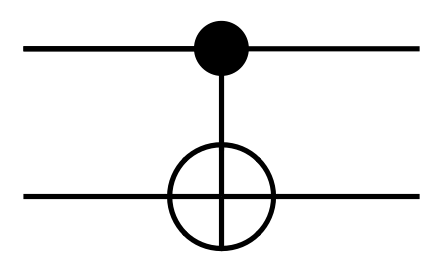
\includegraphics[width=0.15\linewidth]{gfx/CNOT_gate}\\ 
%         Toffoli & $\begin{pmatrix}
%             \mathbb{1}_6 & 0 \\
%             0 & X
%         \end{pmatrix}$ & 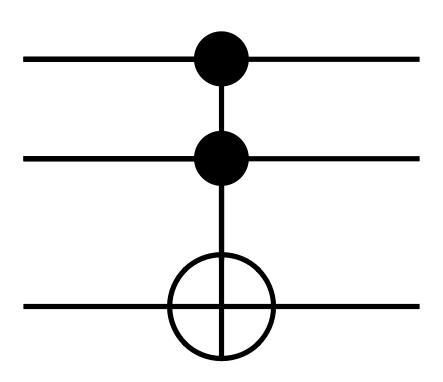
\includegraphics[width=0.15\linewidth]{gfx/Toffoli_gate}\\ 
%         nCNOT & $\begin{pmatrix}
%             \mathbb{1}_{2^n-2} & 0 \\
%             0 & X
%         \end{pmatrix}$ & \\ 
%         H & $\frac{1}{\sqrt{2}}\begin{pmatrix}
%             1 & 1 \\
%             1 & -1
%         \end{pmatrix}$ & 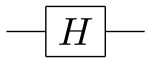
\includegraphics[width=0.15\linewidth]{gfx/150px-Hadamard_gate} \\ 
%         \hline
%     \end{tabular}
%     \caption{Porte logiche quantistiche}
%     \label{table:porte}
% \end{table}



%************************************************
\chapter{Strumenti}\label{ch:strumenti}
%************************************************

Il lavoro per questa tesi è stato svolto principalmente usando un computer 
con sistema operativo GNU/Linux Ubuntu Dell Inspiron 3552 con 8 GB di RAM. 
Per lo sviluppo dei circuiti quantistici si è usato gli strumenti di 
sviluppo e di simulazione messi a disposizione dall'IBM. Questi permettono 
di progettare, simulare ed eseguire su dei quantum computer reali gli 
algoritmi scritti. Il linguaggio di programmazione, sia per l'analisi 
dei dati che per la prototipazione del circuito, è Python; grazie al 
lavoro della comunità open source questo linguaggio si è evoluto 
come strumento omnicomprensivo per una varietà sempre crescente di 
lavori di ricerca scientifica. 

\section{Qiskit}

Qiskit è un'interfaccia di programmazione che permette di scrivere 
circuiti quantistici e simularne l'esecuzione sul proprio computer 
o inviare un ordine di esecuzione a un vero computer quantistico tramite 
l'interfaccia offerta dall'IBM Quantum Experience. 
È consigliata l'esecuzione tramite l'interfaccia Jupyter Notebook per 
la manipolazione dei risultati in tempo reale. 

\section{IBM Q Experience}

L'IBM Q Experience è un servizio offerto gratuitamente da IBM che permette 
a chiunque di avere a che fare con un computer quantistico. Sono presenti 
risorse didattiche per imparare a scrivere il primo circuito, strumenti 
di comunità come una piattaforma di domande e risposte e soprattutto 
un sistema per creare i propri algoritmi. Si può accedere agli ordini di 
esecuzione inviati tramite Qiskit e recuperarne i risultati in un 
secondo momento. 

\section{Esempio di algoritmo}

Come rapido esempio dell'uso di Qiskit si propone il codice che riproduce 
l'algoritmo \ac{QKNN} presentato nella sezione \ref{sec:qknn}.

\begin{lstlisting}[float=h!,language=Python,frame=tb,caption={Algoritmo per il QKNN},label=lst:qknn]
    import qiskit.aqua.circuits.gates.controlled_ry_gates

    a = QuantumRegister(1,'a')
    m = QuantumRegister(1,'m')
    i = QuantumRegister(1,'i')
    c = QuantumRegister(1,'c')
    b = ClassicalRegister(2, 'bit')
    circuit = QuantumCircuit(a,m,i,c,b)

    circuit.h(a)
    circuit.h(m)

    circuit.cry(x0,a[0],i[0])
    circuit.x(a) # swap entanglement with ancilla to 0

    circuit.mcry(t0,a[:]+m[:],i[0],None)
    circuit.x(m) # swap entanglement with m index to 0

    circuit.mcry(t1,a[:]+m[:],i[0],None)

    circuit.cx(m,c) # entangle class 1 with m index 1

    circuit.h(a)
    circuit.measure(a,b[0])
    circuit.measure(c,b[1])

    # circuit.draw(output='mpl')
    \end{lstlisting}

    I valori x0, t0, t1 corrispondono agli angoli di rotazione per il vettore d'input e 
    per i due vettori di training rispettivamente. 
    La porta mcry non si trovava nelle funzioni di base di Qiskit ma è stata importata 
    separatamente attraverso il comando in cima. 
    Il disegno del circuito è presente in appendice nella figura A.1: si può notare 
    come le porte di rotazione controllata siano in realtà realizzate con una sequenza 
    di porte di base più o meno complicata. Tale processo è gestito automaticamente 
    da Qiskit. 
\cleardoublepage
\ctparttext{Implementazione dell'algoritmo k-nearest neighbour e della tecnica 
di costruzione della QRAM; simulazione ed esecuzione su hardware quantistico dei 
circuiti progettati; analisi dei risultati ottenuti.}
\part{Pratica}\label{pt:implementazione}
%************************************************
\chapter{Implementazione multiclasse}\label{ch:implementazione}
%************************************************

\section{Preparazione di uno stato quantistico}

Per analizzare dei dati classici attraverso un computer quantistico 
abbiamo bisogno di codificare in qualche modo le informazioni 
contenute nei nostri insiemi. Nel caso specifico, si parla delle 
coordinate dei vettori nello spazio delle caratteristiche e la 
classe associata ad ognuno di essi. 
Per fare questo, costruiamo degli stati quantistici 
ad hoc che rappresentino i vettori dati in maniera coerente. 
La procedura usata in questa tesi segue la tecnica di costruzione 
\ac{FF-QRAM} proposta da Park, Petruccione e Rhee \cite{petruccione}. 

\subsection{Flip-flop QRAM} \label{sec:ff-qram}

La \ac{FF-QRAM} è usata per memorizzare un \ac{QDB} inizializzato in maniera arbitraria. 
Nell'illustrare l'algoritmo di cotruzione verranno usati due registri quantistici: 
il primo, denotato genericamente $\ket{j}$, o con il pedice $B$, indica quale bus 
di memoria viene usato per il passaggio in corso, mentre il secondo, denotato 
$\ket{b_l}_R$, con il pedice $R$, sarà il registro che contiene i 
valori codificati del vettore dati. 
I vettori $\ket{j}_B$ vengono anche detti appartenere alla base computazionale. 
Lo stato finale dei qubit può essere 
arbitrario e l'ampiezza di probabilità $\psi_j$ con cui è accessibile ciascuno stato 
$\ket{j}_B$ della base computazionale codifica i valori classici di partenza. 

L'operazione QRAM sui qubit bus e registro sovrappone un insieme di dati classici 
$D = \left\{ \left( \vec{d}^{(l)}, b_l \right) | 0 \leq l < M \right\}$, dove 
$\vec{d}^{(l)}$ rappresenta $n$ bit di informazione e $b_l$ è il relativo attributo, come 
\begin{equation} \label{eq:qram}
    \text{QRAM}(D) \sum_j \psi_j \ket{j}_B \ket{0}_R \equiv 
    \sum_l \psi_l \ket{\vec{d}^{(l)}}_B \ket{b_l}_R,
\end{equation}

La \ac{FF-QRAM} è implementata sistematicamente con elementi comuni dei circuiti 
quantistici, che includono la porta di Pauli X controllata classicamente, $\overline{c}X$, 
e la porta di rotazione controllata da $n$ qubit, $C^n R_p (\theta)$. 
La $\overline{c}X$ inverte il qubit bersaglio solo quando il bit classico di 
controllo è zero. La porta $C^n R_p (\theta)$ ruota il qubit bersaglio di $\theta$ attorno 
all'asse $p$ della sfera di Bloch solo se tutti gli $n$ qubit sono 1. 

\begin{figure}[ht]
    \centering
    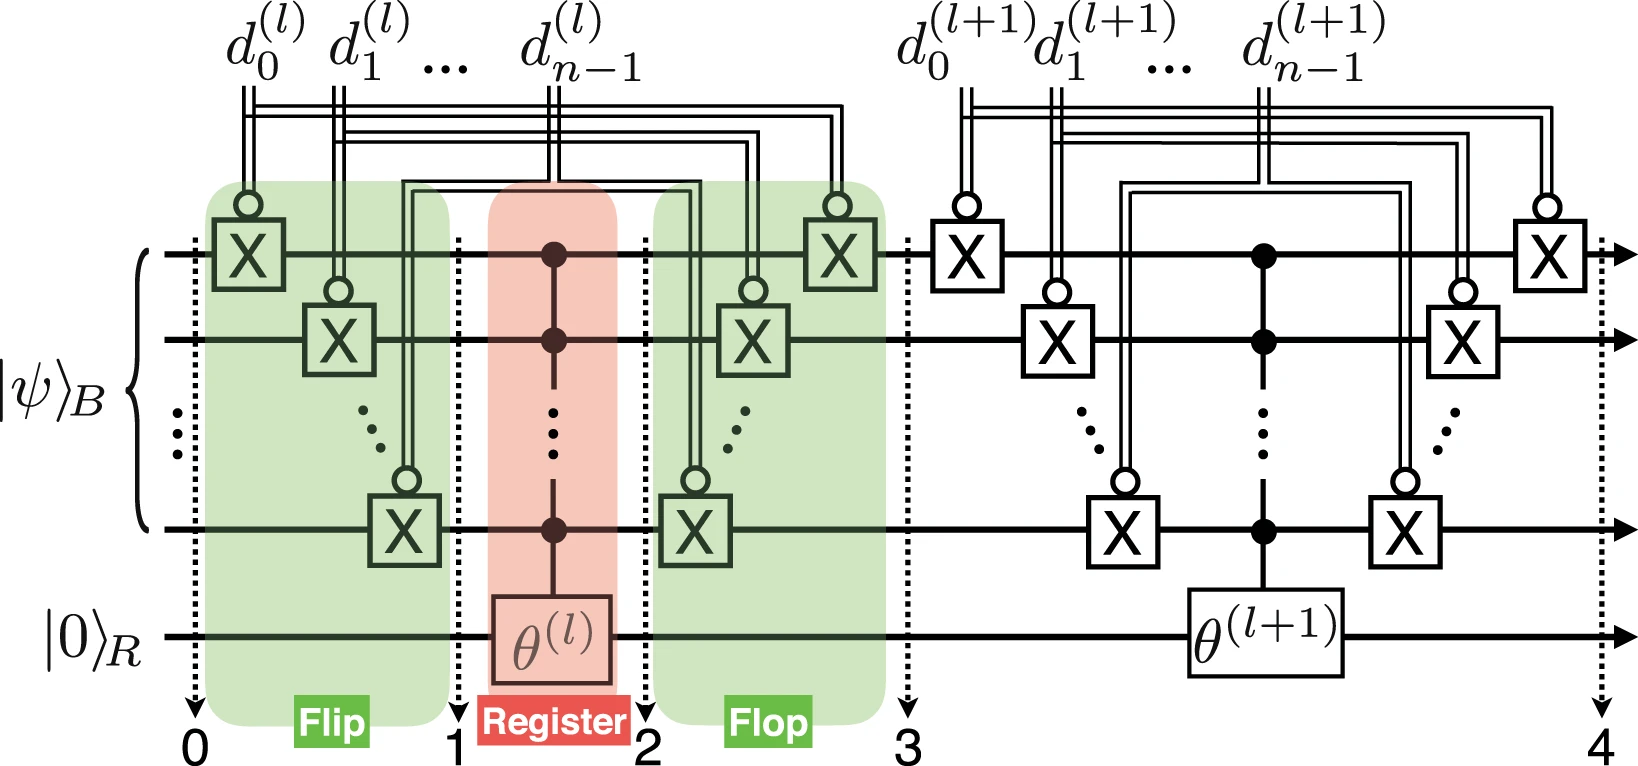
\includegraphics[width=\linewidth]{gfx/qram}
    \caption[Procedimento di costruzione FF-QRAM]%
    {Procedimento di costruzione FF-QRAM \par \small 
    Circuito quantistico per \ac{FF-QRAM} che scrive
    le stringhe di bit $\vec{d}^{(l)}$ e $\vec{d}^{(l+1)}$ 
    come una sovrapposizione di stato quantistico con ampiezze 
    di probabilità determinate da $\theta^{(l)}$ e $\theta^{(l+1)}$ 
    rispettivamente, usando porte di rotazione controllate da più qubit. 
    Le linee doppie indicano operazioni controllate classicamente, 
    ed il cerchio vuoto (pieno) indica che la porta è attivata quando il 
    bit (qubit) di controllo è 0 (1). Le frecce tratteggiate e numerate 
    indicano i vari passaggi descritti nel testo principale.}
    \label{fig:qram}
\end{figure}

L'idea soggiacente al modello della \ac{FF-QRAM} è rappresentata in figura \ref{fig:qram}, 
che descrive la procedura per sovrapporre due stringhe di bit indipendenti 
$\vec{d}^{(l)}$ e $\vec{d}^{(l+1)}$ con ampiezze di probabilità desiderate 
nello stato del qubit bus $\ket{\psi}_B$. 
Lo stato iniziale può essere espresso focalizzandosi su $\vec{d}^{(l)}$ come 
\begin{equation}
    \ket{\psi_0}_l = \psi_{\vec{d}^{(l)}} \ket{\vec{d}^{(l)}} \ket{0}_R + \sum_{j \neq \vec{d}^{(l)}} 
    \psi_j \ket{j} \ket{0}_R,
\end{equation}
dove $\ket{\psi_s}_l$ denota lo stato degli ($n$) qubit nel processo di 
scrittura dell'$l$-esimo valore dati, osservato all'$s$-esimo passo in figura \ref{fig:qram}. 

Le porte $\overline{c}X$ controllate da $\vec{d}^{(l)}$ risistemano gli stati 
della base computazionale dei qubit bus cosicché $\ket{\vec{d}^{(l)}}$ diventa 
$\ket{1}^{\otimes n}$, ed il resto dei bit quantistici si invertono di conseguenza: 
\begin{equation}
    \ket{\psi_1}_l = \psi_{\vec{d}^{(l)}}\ket{1}^{\otimes n} \ket{0}_R + 
    \sum_{\ket{\overline{j \oplus \vec{d}^{(l)}}} \neq \ket{1}^{\otimes n} } \psi_j \ket{\overline{j \oplus \vec{d}^{(l)}}} 
    \ket{0}_R.
\end{equation}
La sovralinea nell'ultimo termine indica che l'inversione del bit avviene se il 
bit di controllo è 0. Dopo il passo 1, la rotazione controllata dai qubit, 
$C^n R_y(\theta^{(l)})$, denotata come $\theta^{(l)}$ nella figura, è applicata 
al qubit registro. Lo stato quantistico al passo 2 diventa 
\begin{equation}
    \ket{\psi_2}_l = \psi_{\vec{d}^{(l)}} \ket{1}^{\otimes n} \ket{\theta^{(l)}}_R + 
    \sum_{\ket{\overline{j \oplus \vec{d}^{(l)}}} \neq \ket{1}^{\otimes n} } \psi_j \ket{\overline{j \oplus \vec{d}^{(l)}}} 
    \ket{0}_R,
\end{equation}
dove $\ket{\theta}=\cos\theta\ket{0}+\sin\theta\ket{1}$. 
Le porte $\overline{c}X$ condizionate da $\vec{d}^{(l)}$ sono applicate di nuovo 
per far ritornare alla condizione precedente lo stato dei bus: 
\begin{equation}
    \ket{\psi_3}_l = \psi_{\vec{d}^{(l)}} \ket{\vec{d}^{(l)}} \ket{\theta^{(l)}}_R + 
    \sum_{j \neq \vec{d}^{(l)}} \psi_l \ket{j} \ket{0}_R.
\end{equation}

Il secondo giro registra i dati successivi di $\vec{d}^{(l+1)}$ e $\theta^{(l+1)}$: 
\begin{equation}
    \begin{split}
        &\ket{\psi_4}_{l,l+1} = \psi_{\vec{d}^{(l)}} \ket{\vec{d}^{(l)}} \ket{\theta^{(l)}}_R + \\
        &+ \psi_{\vec{d}^{(l+1)}} \ket{\vec{d}^{(l+1)}} \ket{\theta^{(l+1)}}_R + 
        \sum_{j \neq \vec{d}^{(l)},\vec{d}^{(l+1)}} \psi_j \ket{j} \ket{0}_R.
    \end{split}
\end{equation}
Questo processo può essere ripetuto tante volte quanti sono i dati da inserire. 
In questo modo, $M$ valori possono essere registrati con pesi non uniformi per 
generare lo stato 
\begin{equation}
    \sum_{l=0}^{M-1} \psi_{\vec{d}^{(l)}} \ket{\vec{d}^{(l)}} \left[ \cos\theta^{(l)} 
    \ket{0}_R + \sin\theta^{(l)} \ket{1}_R \right] + 
    \sum_{j \notin \{ \vec{d}^{(l)} \}} \psi_j \ket{j} \ket{0}_R.
\end{equation}
Infine, il \ac{QDB} richiesto nell'eq. \ref{eq:qram} può essere ottenuto 
selezionando un angolo $\theta^{(l)}$ appropriato che sia legato all'ampiezza di 
probabilità desiderata $b_l$, e postselezionando il risultato di misura $\ket{1}_R$. 
La probabilità di misurare $\ket{1}_R$ è 
\begin{equation} \label{eq:qram.prob}
    P(1) = \sum_{l=0}^{M-1} |\psi_{\vec{d}^{(l)}} \sin\theta^{(l)} |^2.
\end{equation}
Il costo per preparare uno stato con questo procedimento è di 
$\mathcal{O}(n)$ qubit e $\mathcal{O}(Mn)$ operazioni quantistiche. 

\section{Approccio multiclasse}

L'algoritmo \ac{QKNN} presentato in sezione \ref{sec:qknn} è stato implementato 
su un computer a 5 qubit, di cui solo 4 sono stati usati. La codifica usata prevedeva 
che un vettore bidimensionale $x = (x_0,x_1)$ normalizzato fosse codificato nello stato del 
qubit $\ket{i}$ come $\ket{psi_x} = x_0 \ket{0} + x_1 \ket{1}$ attraverso una rotazione 
controllata dai qubit $\ket{a}$ e $\ket{m}$. Si faccia riferimento alla figura 
\ref{fig:circuito_schuld}. Parametrizzando l'angolo di Bloch attraverso la relazione 
\begin{equation}
    x_0 = \cos(\theta), \quad x_1 = \sin(\theta),
\end{equation}
otteniamo la relazione tra i vettori d'input e l'angolo $\theta$
\begin{equation}
    \theta = \arctan\frac{x_1}{x_0}. 
\end{equation}

\begin{figure}[h]
    \centering
    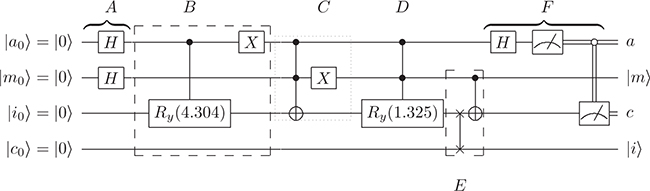
\includegraphics[width=\linewidth]{gfx/schuld_circuito}
    \caption{Il circuito quantistico base per il QKNN}
    \label{fig:circuito_schuld}
\end{figure}

La relazione appena mostrata è una delle prime che verranno modificate per permettere 
l'uso della \ac{QRAM}, quando si vorranno inserire vettori di dimensione maggiore di 2. 

Infatti, facendo riferimento all'eq. \ref{eq:qram.prob}, troviamo che lo stato costruito 
dopo la misura condizionale è 
\begin{equation}
    \sum_{l=0}^{M-1} \psi_{\vec{d}^{(l)}}\ket{\vec{d}^{(l)}}\sin\theta^{(l)}\ket{1}_R. 
\end{equation}
La relazione esistente tra i valori $b_l$, ovvero le componenti $x_i$, 
e le ampiezze di probabilità nella \ac{QRAM} è allora
\begin{equation} \label{eq:angolo.qram}
    \theta = \arcsin x_i. 
\end{equation}

L'espansione delle capacità del circuito prevede dunque l'aumento dei qubit 
dedicati a ciascun registro quantistico tra i seguenti: 
\begin{itemize}
    \item al registro $\ket{m}$ per aumentare i vettori di apprendimento; 
    \item al registro $\ket{i}$ per aumentare la dimensionalità dei vettori; 
    \item al registro $\ket{c}$ per aumentare il numero di classi riconosciute. 
\end{itemize}
Lo schema circuitale passa da quello mostrato in figura \ref{fig:circuito_schuld} a 
quello più generico mostrato in figura \ref{fig:qram_classi}. 

\begin{figure}[h!]
    \centering
    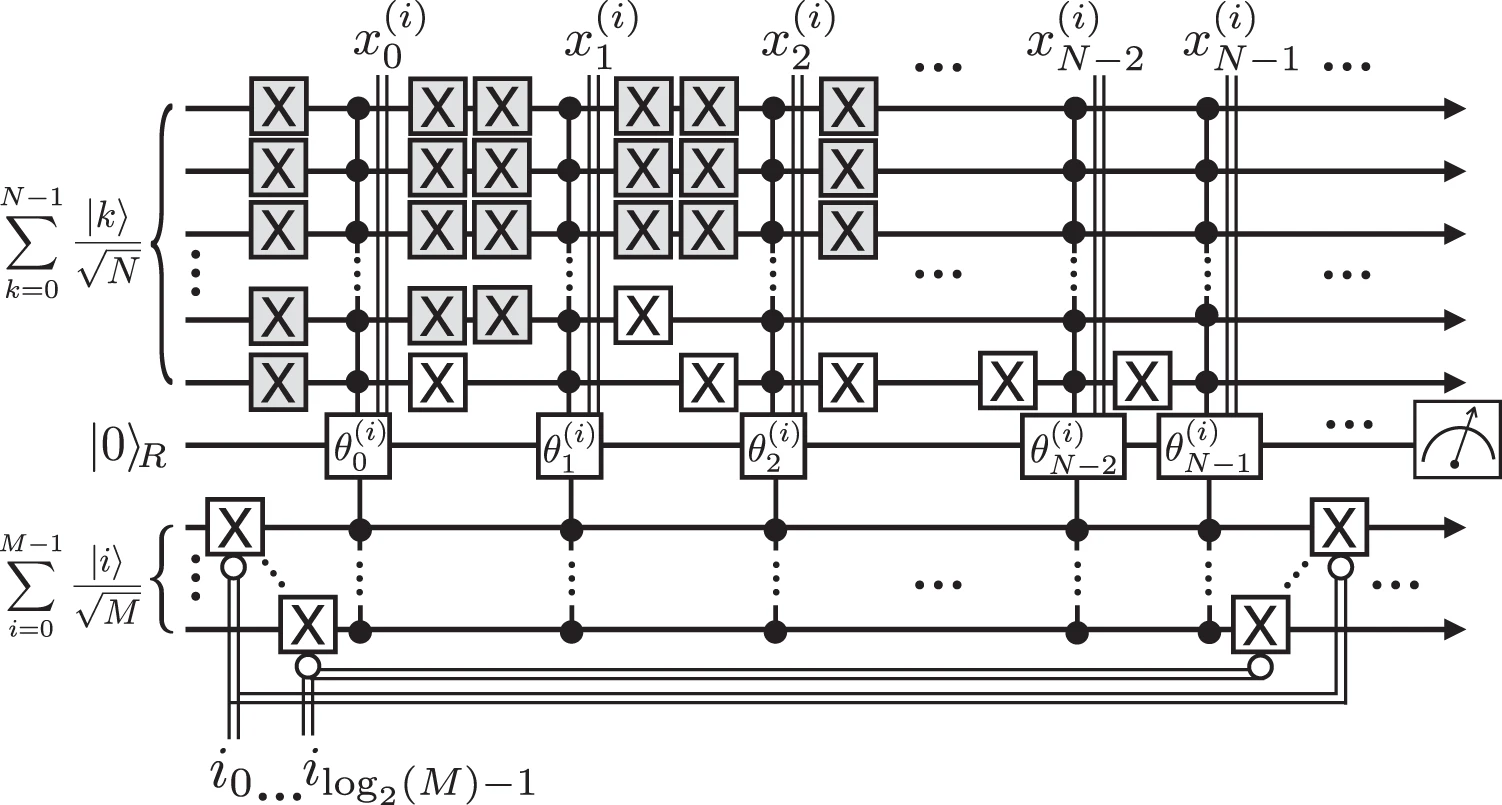
\includegraphics[width=\linewidth]{gfx/qram_classi}
    \caption[Circuito quantistico per preparare il \acs{QDB} per un quantum support vector machine]%
    {Circuito quantistico per preparare il \acs{QDB} per un quantum support vector machine. \par \small 
    Sono mostrate le porte per scrivere solo l'$i$-esimo vettore di apprendimento. Le porte ombreggiate 
    in grigio sono aggiunte esclusivamente per illustrare il processo flip-flop, e non sono implementate 
    in pratica.}
    \label{fig:qram_classi}
\end{figure}

La codifica del vettore d'input prevede che i qubit di controllo siano solo quelli mostrati 
nella parte superiore della figura. Al contrario, quando si codificano i vettori di 
apprendimento, li si pone in entanglement anche con i qubit indice $\ket{m}$ e 
classe $\ket{c}$, applicando le opportune porte $\overline{c}X$ all'inizio ed alla 
fine della loro codifica. 

Adottando una configurazione di esempio con 2 qubit indice, 2 qubit caratteristica e 
2 qubit classe si ottiene un classificatore capace di confrontare un vettore di 
input con 4 vettori di apprendimento aventi 4 caratteristiche ed appartenenti a 4 classi. 
Si riporta il codice relativo a tale realizzazione nel riquadro \ref{lst:multiclasse}. 

\begin{lstlisting}[float=h!,language=Python,frame=tb,caption={Algoritmo per il QKNN multiclasse},label=lst:multiclasse]
    a = QuantumRegister(1,'a') # knn ancilla
    m = QuantumRegister(2,'m') # training vector index
    i = QuantumRegister(2,'i') # feature index
    r = QuantumRegister(1,'r') # rotation qubit
    q = QuantumRegister(5,'q') # qram ancilla
    c = QuantumRegister(2,'c') # class
    b = ClassicalRegister(4, 'bit')
    circuit = QuantumCircuit(a,m,i,r,q,c,b)

    circuit.h(a)
    circuit.h(m)
    circuit.h(i)
    circuit.h(c)

    # circuit.cry(theta, control, target)
    # circuit.mcry(theta, controls, target, ancillae)

    # >>> Encode the input vector >>>

    encodeVector(circuit,inputVirginica,i,a[:]+i[:],r[0],q)

    circuit.x(a) # swap entanglement with ancilla to 0

    # <<< Encode the input vector <<<

    # >>> Encode the training vectors >>>

    buildTrainingState(trainingArray)

    # <<< Encode the training vectors <<<

    circuit.measure(r,b[0])

    circuit.h(a)

    circuit.measure(a,b[1])
    circuit.measure(c[0],b[2])
    circuit.measure(c[1],b[3])
\end{lstlisting}

La funzione \texttt{buildTrainingState} prende i vettori appartenenti a \texttt{trainingArray} 
e ne codifica i valori nelle ampiezze dei qubit attraverso la funzione mostrata 
nel riquadro \ref{lst:encodeTraining}. 

\begin{lstlisting}[float=h!,language=Python,frame=tb,caption={Funzione per codificare i vettori},label=lst:encodeTraining]
    def encodeTraining(circuit,data,i,controls,rotationQubit,ancillaQubits,c,m):
    # Header
    encodeClass(circuit,c)
    encodeIndex(circuit,m)
    
    # Encoder
    encodeVector(circuit,data,i,controls,rotationQubit,ancillaQubits)
    
    # Footer
    encodeClass(circuit,c)
    encodeIndex(circuit,m)
\end{lstlisting}

Le funzioni nell'header e nel footer altro non fanno che applicare le giuste porte X, 
come descritto in sezione \ref{sec:ff-qram} e in figura \ref{fig:qram_classi}. 
Più nello specifico, la funzione \texttt{encodeVector} applica le porte della parte 
superiore dell'immagine ed effettua le rotazioni controllate, 
mentre \texttt{encodeClass} e \texttt{encodeIndex} applicano 
quelle della parte inferiore\footnote{Per accedere al codice completo, fare riferimento 
alla cartella Script nella repository su GitHub \url{https://github.com/visika/Tesi}}. 

Nel capitolo successivo si discutono i risultati di classificazione ottenuti in 
caso di simulazione ed esecuzione su hardware quantistico. 

% Il quantum-enhanced machine learning (QEML) prova a rispondere alla domanda 
% se le proprietà quantomeccaniche come il parallelismo quantistico, 
% l'interferenza e i concetti di informazione quantistica possano essere usati 
% per migliorare gli algoritmi di machine learning classico. Il QEML è un campo 
% di ricerca relativamente nuovo, dimostrato dal fatto che il termine 
% \emph{quantum machine learning} è stato coniato solo nel 2013 in un manoscritto 
% di Lloyd, Mohseni e Rebentrost (2013). % inserire fonte *******************
% Dal 1995 in poi, molti algoritmi di QEML sono stati pubblicati, come riassunto 
% nel recente articolo di revisione di Biamonte et al. (2016). % inserire fonte **
% Per ottenere accelerazioni quantistiche, molti algoritmi di QEML usano procedure
% quantistiche ben note, come l'algoritmo di ricerca di Grover, la trasformata di 
% Fourier quantistica o la quantum phase estimation come sottoprocessi per compiti
% di machine learning più grandi. % inserire fonti **********************

% Il machine learning classico prende dati classici in entrata ed impara da essi 
% usando algoritmi classici eseguiti su computer classici: Aïmeur % aggiungi fonti
% si riferiscono a questo come C/C (dati classici con algoritmi classici). 
% Si entra nel campo del \ac{MLQ} generico quando uno tra dati quantistici e 
% algoritmi quantistici è combinato con il machine learning. Ebbene, Aïmeur 
% % aggiungi fonti *************************************
% dividono il campo del machine learning quantistico in tre diversi sottocampi: 
% \begin{itemize}
%     \item C/Q: dati classici con algoritmi quantistici;
%     \item Q/C: dati quantistici con algoritmi classici;
%     \item Q/Q: dati quantistici con algoritmi quantistici.
% \end{itemize}
% Così, i dati quantistici includono qualsiasi dato descrivente un sistema 
% quantomeccanico come p.e. l'hamiltoniana o il vettore d'onda di un sistema 
% quantistico.

% Il sottocampo Q/C elabora dati quantistici con algoritmi di machine learning 
% classico. Per esempio, Carrasquilla e Melko (2016) % aggiungi fonti *******
% hanno usato il pacchetto di deep learning TensorFlow di Google per identificare 
% transizioni di fase in sistemi quantistici. Il sottocampo Q/Q è l'unione di 
% C/Q e Q/C e ha a che fare con l'elaborazione di dati quantistici attraverso 
% l'uso di algoritmi quantistici p.e. imparare come è fatta l'hamiltoniana di un 
% sistema quantistico unsando algoritmi di machine learning quantistico. Questo 
% lavoro di tesi è immerso nel sottocampo C/Q, anche chiamato QEML, che mira a 
% sviluppare algoritmi quantistici per compiti di machine learning che coinvolgono 
% dati classici. 

% Le sezioni seguenti introdurranno alcuni dei concetti fondamentali dal campo 
% del QEML. Più nello specifico, la sezione 4.2 % rivedere ********************
% presenta la versione quantistica dell'algoritmo k-nn classico, la cui simulazione
% ed esecuzione quantistica saranno discussi nel capitolo 5. 
% % Quindi il capitlo 5 discuterà i risultati
% In ogni caso, dato che un algoritmo quantistico è una sequenza di porte 
% quantistiche, può solo manipolare bit quantistici e non classici. 
% Dunque, la prossima sezione descriverà prima come dei dati classici possano 
% essere trasferiti in degli stati quantistici, in modo da permettere 
% l'elaborazione quantistica. 

% La preparazione di uno stato quantistico è il procedimento in cui si prepara 
% uno stato quantistico che rappresenta accuratamente un vettore contenente 
% dati classici (normalizzati). Per applicare qualsiasi algoritmo di machine 
% learning quantistico a dati classici, la preparazione dello stato quantistico 
% deve sempre essere eseguita prima. Perciò, bisogna diventare familiari 
% con le nozioni di preparazione degli stati quantistici prima di procedere nelle 
% sezioni avanzate di questa tesi. Ci sono due modi fondamentalmente diversi 
% di codificare dei dati classici in stati quantistici ma in questa tesi ne verrà 
% usato solo uno. Il primo modo consiste nel codificare lo stato dei bit classici 
% che appartengono ai nostri dati direttamente negli stati dei singoli qubit: 
% al bit 0 viene fatto corrispondere un qubit nello stato $\ket{0}$ ed al bit 1 
% un qubit nello stato $\ket{1}$. Una ricetta per effettuare una tale operazione 
% è descritta da Trugenberger (2001). % inserisci fonte ******************
% Una maniera più raffinata di rappresentare un vettore classico come uno stato 
% quantistico, che è quella che verrà adottata, sfrutta le $2^n$ ampiezze di un 
% sistema di $n$ qubit. In questo modo un vettore $k$-dimensionale può essere 
% codificato usando solo $\log_2(k)$ qubit, poiché abbiamo visto che il numero 
% di ampiezze disponibili cresce esponenzialmente con il numero dei qubit. 
% Questo tipo di memorizzazione dei dati apre le porte ad una compressione 
% esponenziale dei dati classici. 

% Se si ha un vettore classico e lo si vuole codificare nelle ampiezze si può fare 
% la seguente operazione 
% \begin{equation}
%     \begin{pmatrix}
%         0.6\\0.4
%     \end{pmatrix}
%     \arrowvert
%     \ket{n} = \sqrt{0.6}\ket{0} + \sqrt{0.4}\ket{1}.
% \end{equation}

% Se abbiamo un insieme di M dati classici rappresentati come 
% % $D = \{ (\vec{d}^{(l)}), b_l \} | 0 \leq l < M}$, dove $\vec{d}^{(l)}$ rappresenta 
% n bit di informazione, ovvero l'indirizzo del registro, a cui è associato il dato 
% $b_l$ (che può essere un valore binario o reale), possiamo costruire uno stato 
% quantistico che soddisfi la seguente relazione: 
% \begin{equation} \label{eq:qdb}
%     % \ket{\psi}_{QDB} = \sum_{l=0}^{M-1}b_l\ket{\vec{d}^{(l)}}
% \end{equation}
% QDB è quantum database. 
% Stiamo dicendo che conserviamo ogni valore $b_l$ in una ampiezza dei qubit a disposizione. 

% commento sulla postselezione **********************

% continua a inserire dall'articolo ***********************************

% I dettagli tecnici verranno descritti nella appendice. 

% si potrebbe dire che cos'è una QRAM

%************************************************
\chapter{Risultati e discussione}\label{ch:risultati}
%************************************************

% ***********************************************
% [ ] Mettere i grafici con le tre classi
% ***********************************************

Per l'implementazione dell'algoritmo è stato scelto il ben noto 
data set Iris, consistente in una tabella di lunghezze e larghezze 
del petalo e del sepalo collegate a tre specie di fiore Iris. 
Come evidenziato in Schuld et al. \cite{schuld}, 
l'insieme dati si è dovuto standardizzare e 
normalizzare prima dell'utilizzo. 
Il passo successivo è stato ripetere l'esperienza dell'articolo 
per comprenderne appieno il funzionamento e poterlo estendere. 
Questa tesi parte dalla situazione base, in cui
si usano due caratteristiche delle 
quattro disponibili, due vettori di apprendimento 
e si possono classificare solo due classi alla volta. 
Questa versione esemplificativa è stata fatta girare con successo 
sul processore quantistico a 5 qubit messo a disposizione dall'IBM.
Di fronte alla disponibilità di un nuovo computer quantistico a 16 
qubit\footnote{\url{https://developer.ibm.com/dwblog/2017/quantum-computing-16-qubit-processor/}, 
Recuperato l'8 settembre 2019}, 
ci si chiede quali sono le prossibilità di miglioramento delle 
implementazioni pratiche. Si è lavorato sulle seguenti proprietà: 
\begin{itemize}
    \item aumentare il numero di classi riconosciute;
    \item aumentare il numero di caratteristiche considerate;
    \item aumentare il numero di vettori di training.
\end{itemize}
Per fare ciò, si è dovuto tenere in considerazione i compromessi 
in termini di numero di qubit ed efficienza di classificazione: 
infatti, per realizzare ognuno di questi punti c'è bisogno di impegnare 
più qubit, non solo per una questione di memoria, ma anche per 
la complessità delle operazioni da effettuare; un'esempio è dato 
dalla porta $C^n R_y (\theta)$, usata nel procedimento di costruzione 
della \ac{QRAM} (vedi sezione \ref{sec:ff-qram}), che necessita di un 
qubit ancilla in più per ogni qubit di controllo aggiuntivo. 

\section{Ottimizzazione dei dati}

Il data set Iris completo si presenta nella forma mostrata in figura 
\ref{fig:iris_grezzi}, dove sono indicate le prime due caratteristiche 
sugli assi coordinati. 

\begin{figure}[ht]
    \centering
    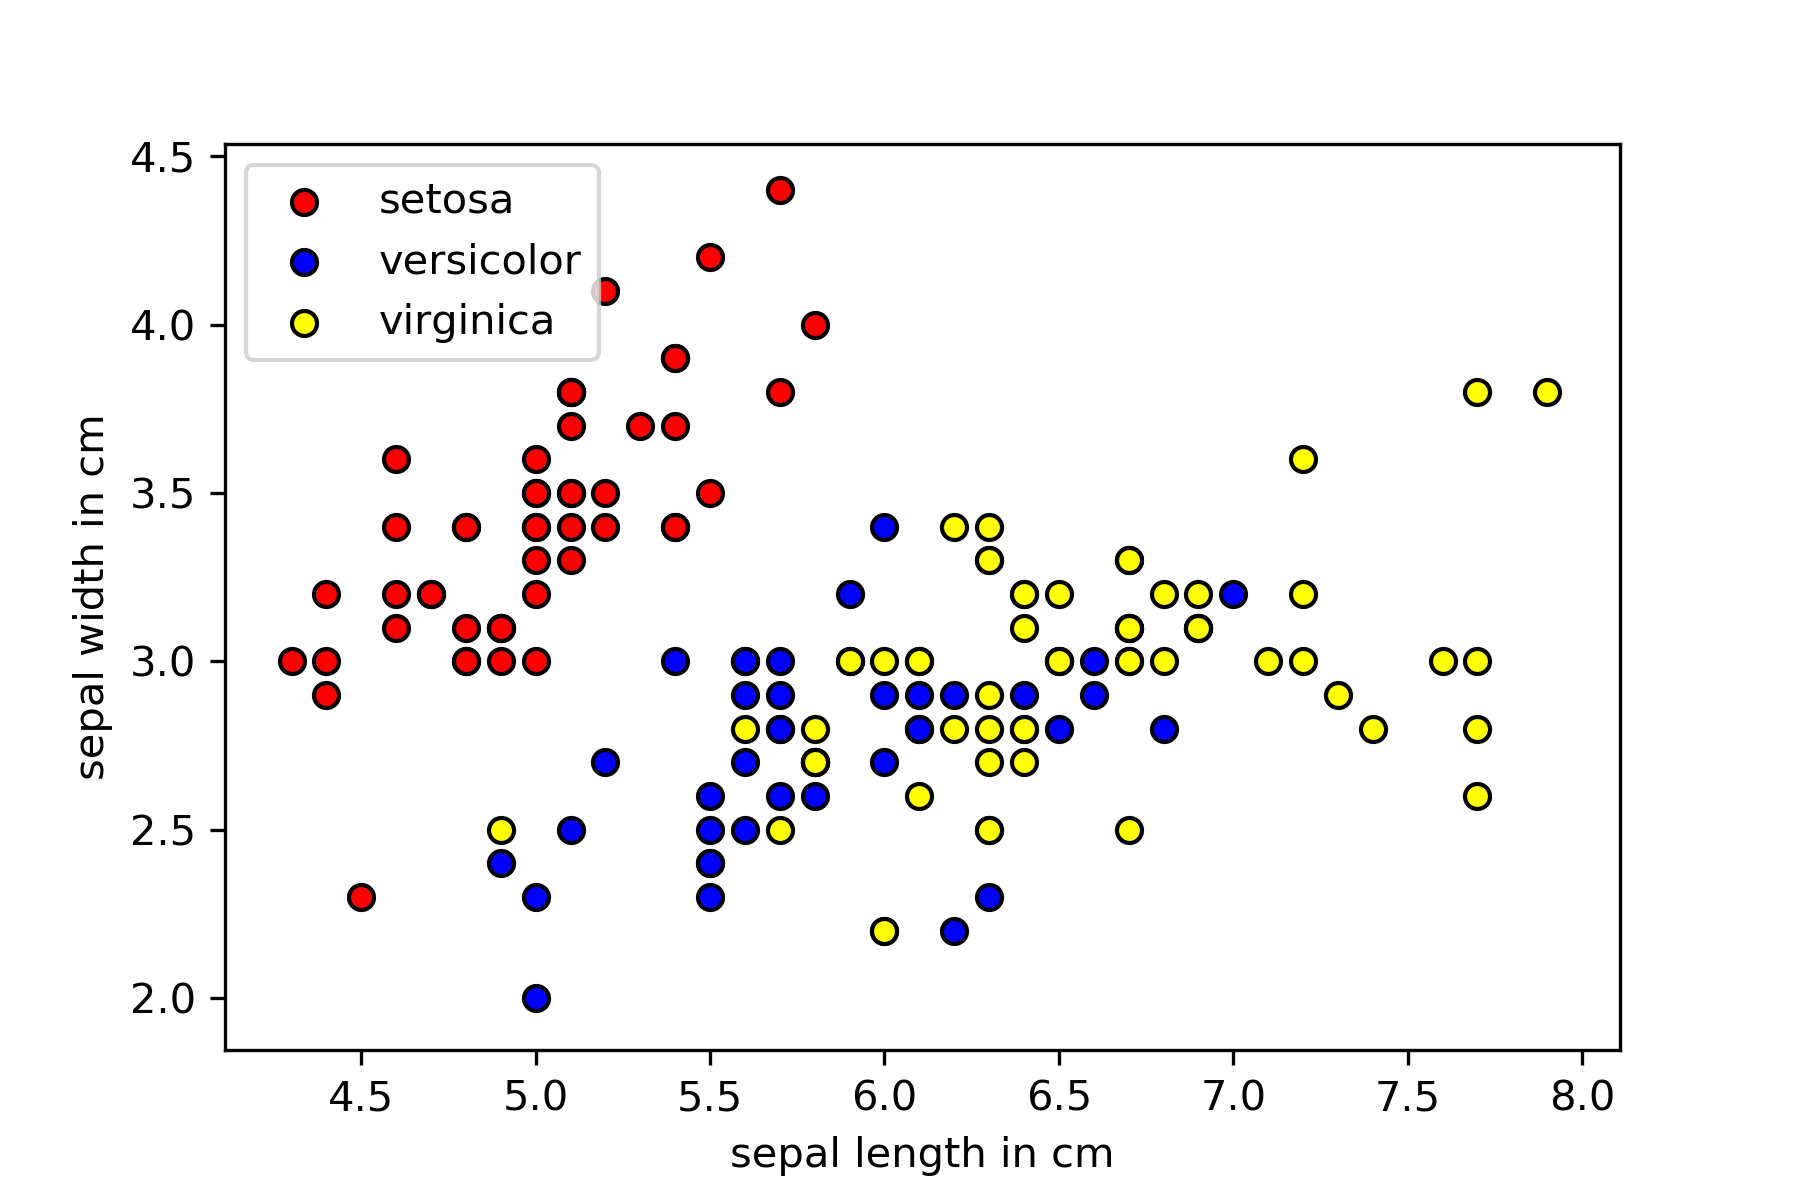
\includegraphics[width=\linewidth]{gfx/iris/irisfeatures}
    \caption{Data set Iris non elaborato}
    \label{fig:iris_grezzi}
\end{figure}

La prima operazione sui dati è la standardizzazione, che trasla e scala 
i punti in modo che abbiamo media nulla e deviazione standard unitaria. 
Si possono notare gli effetti nella figura \ref{fig:iris_standard}, 
osservando i nuovi valori sugli assi. 

\begin{figure}[h!]
    \centering
    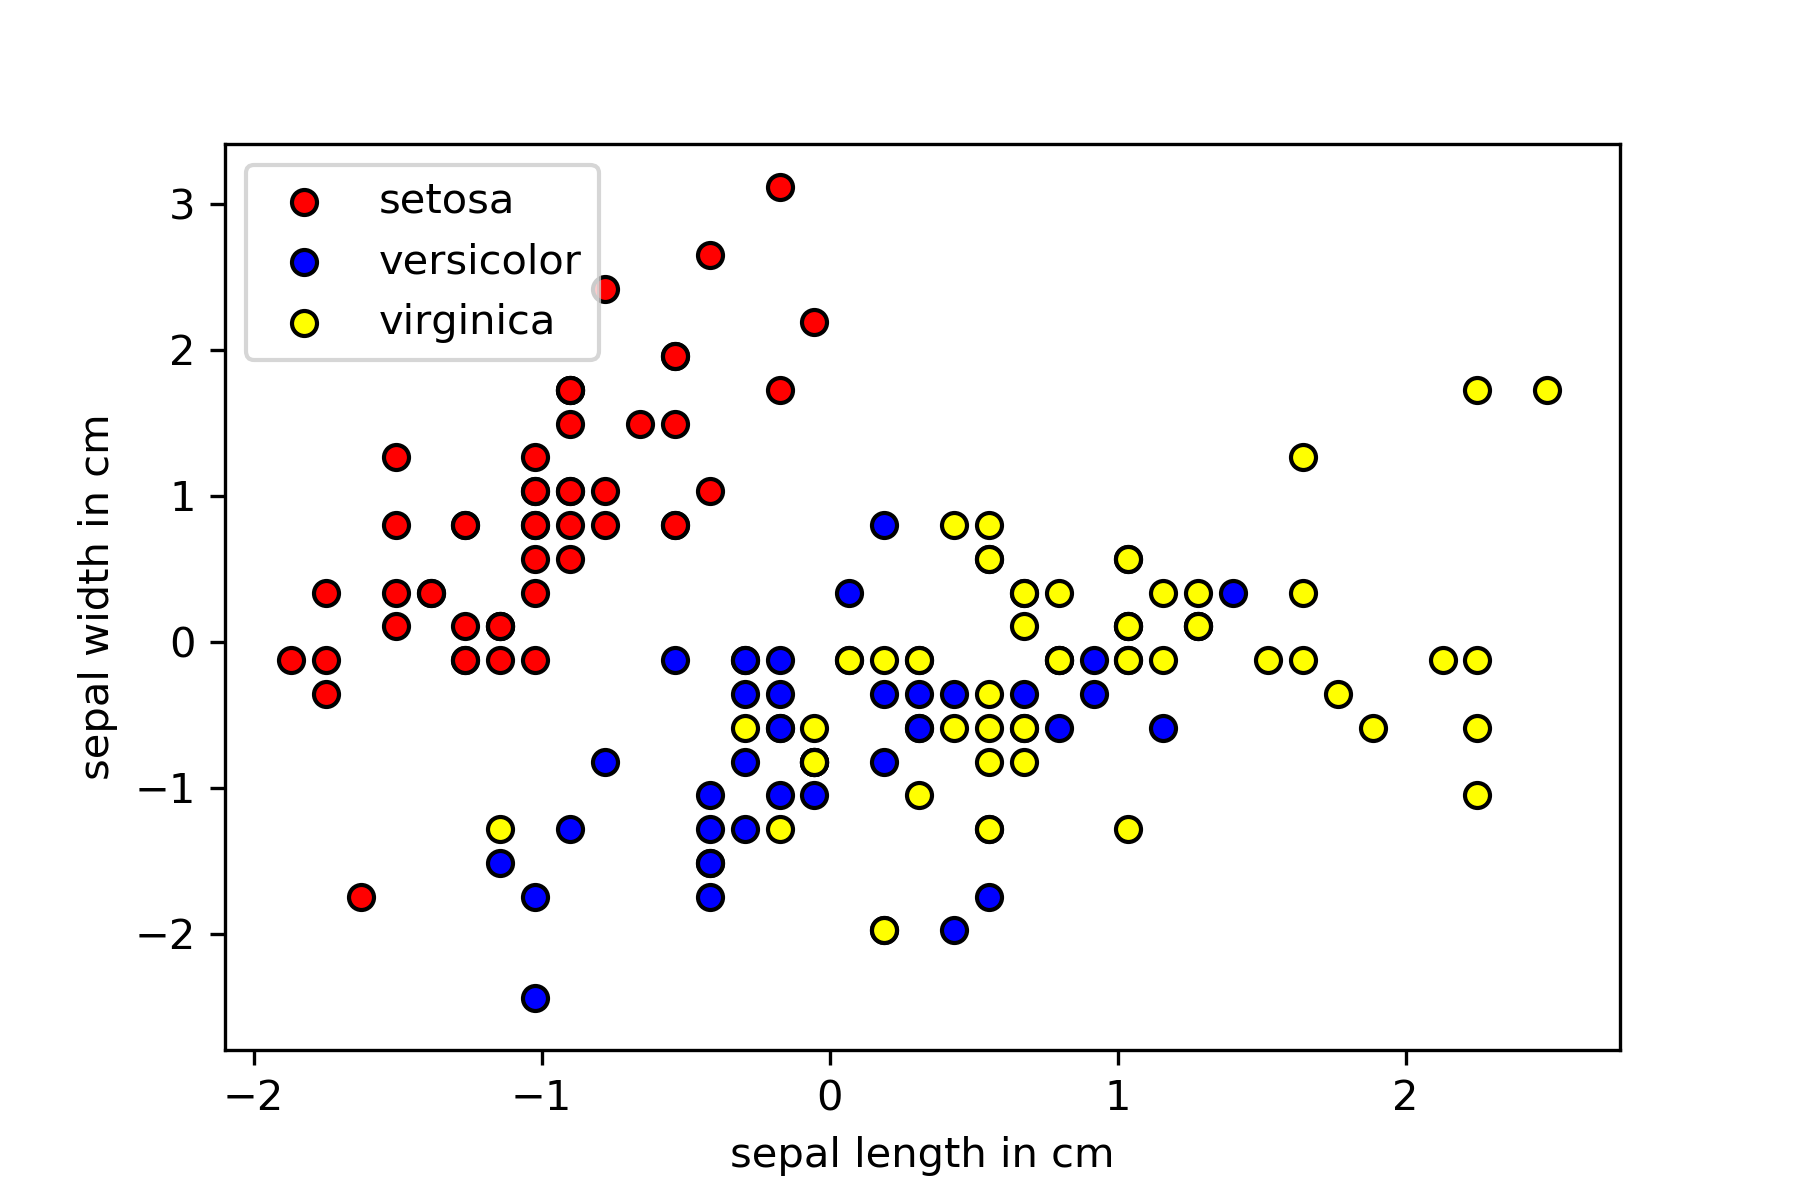
\includegraphics[width=\linewidth]{gfx/iris/irisscaled}
    \caption{Data set Iris standardizzato}
    \label{fig:iris_standard}
\end{figure}

La normalizzazione termina il processo preliminare di ottimizzazione 
dei dati. Si può vedere l'effetto della normalizzazione su un data set 
con due caratteristiche in figura \ref{fig:iris_normal}. 

\begin{figure}[ht]
    \centering
    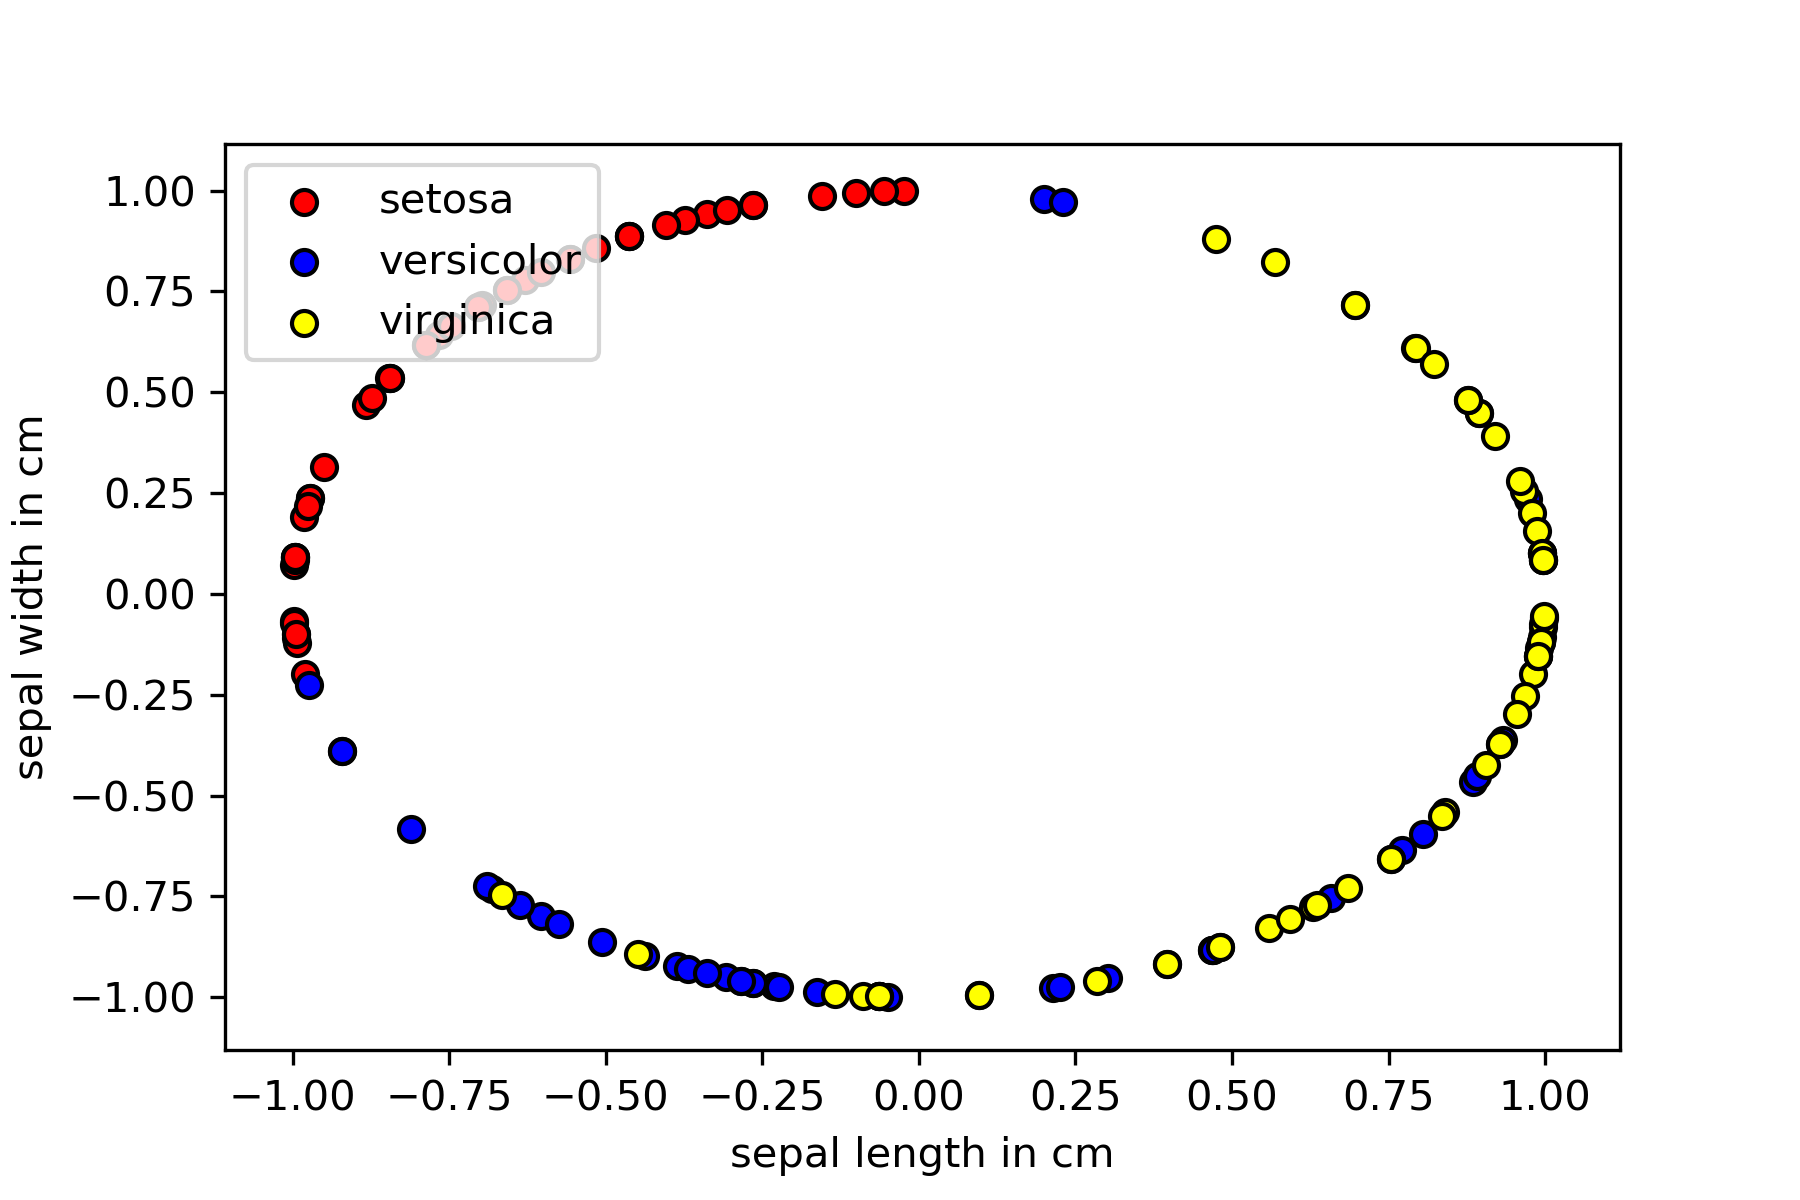
\includegraphics[width=\linewidth]{gfx/iris/irisnormalized}
    \caption{Data set Iris normalizzato}
    \label{fig:iris_normal}
\end{figure}

Avendo effettuato queste operazioni, si deve ora tradurre le coordinate 
di ciascun vettore nello spazio delle caratteristiche in un angolo di rotazione 
da applicare al qubit registro della \ac{QRAM}. 

Facendo riferimento all'eq. \ref{eq:qram.prob}, troviamo che lo stato costruito, 
dopo la misura condizionale, è 
\begin{equation}
    \sum_{l=0}^{M-1} \psi_{\vec{d}^{(l)}}\ket{\vec{d}^{(l)}}\sin\theta^{(l)}\ket{1}_R. 
\end{equation}
La relazione esistente tra i valori $b_l$, ovvero le caratteristiche standardizzate e normalizzate, 
e le ampiezze di probabilità nella \ac{QRAM} è 
\begin{equation}
    \theta^{(l)} = \arcsin b_l. 
\end{equation}

\section{Scrittura dell'algoritmo}

Avendo acquisito le nozioni teoriche e i parametri iniziali, si prova 
adesso a costruire il circuito quantistico attraverso le porte 
dell'insieme universale di base, disponibili grazie all'interfaccia IBM 
Q Experience ed al kit di sviluppo Qiskit. 

Seguendo la figura A.1 in appendice, si 
esamina il circuito quantistico di base: 
\begin{enumerate}
    \item i qubit ancilla ed indice vengono posti in sovrapposizione uniforme; 
    \item il vettore d'input $x$ è posto in entanglement con lo stato fondamentale 
    dell'ancilla;
    \item il vettore di training $t^0$ è posto in entanglement con lo stato eccitato 
    dell'ancilla e con lo stato fondamentale del qubit indice;
    \item il vettore di training $t^1$ è posto in entanglement con lo stato eccitato 
    dell'ancilla e del qubit indice;
    \item il qubit classe è invertito condizionato dal fatto che il qubit indice sia $\ket{1}$; 
    questo completa la preparazione iniziale dello stato; 
    \item nell'ultimo passaggio la porta Hadamard fa interferire le copie di $x$ con i vettori 
    d'apprendimento e l'ancilla è misurata, seguita da una misura del qubit classe. 
\end{enumerate}
Considereremo validi per i nostri scopi solo le misure del qubit classe ottenute quando il 
qubit ancilla è trovato nello stato $\ket{0}$. 
Possiamo notare, tra le altre cose, che la porta $C^n R_y (\theta)$ è in 
realtà formata da una successione di più porte di base. Mentre nei primi tempi 
era necessario inserire manualmente i singoli elementi logici per eseguire una operazione 
complessa, nella realizzazione attuale si è sfruttato il lavoro della comunità 
open source di Qiskit, che ha messo a disposizione comandi veloci per aggiungere 
facilmente porte multi controllate. 

\subsection{Classificazione iniziale}

Si mostra un esempio di risultato di classificazione usando le prime due caratteristiche 
del data set e gli elementi appartenenti alle classi setosa e versicolor. 
Si scelgono come vettori di training un elemento per ciascuna classe, nel nostro caso 
il vettore 34 ed il vettore 86 dal data set, rispettivamente setosa e versicolor. 
Si assegna alla classe setosa lo stato $\ket{0}$ del qubit classe ed alla classe 
versicolor lo stato $\ket{1}$. 
Si sottopongono poi a classificazione, in due esperimenti separati, due vettori sconosciuti: 
il vettore 29 (setosa) ed il vettore 57 (versicolor). 

Il primo passo è simulare l'esperimento sul computer in uso, dato che il problema in esame
è facilmente eseguibile su un comune portatile. I risultati non filtrati per i due esperimenti 
sono visibili nel riquadro \ref{fig:simulazione_circuito}. Nella didascalia sono scritti i conteggi corrispondenti ad un 
determinato esito di misura sui due qubit ancilla e classe. La cifra sulla destra contiene la 
misura del qubit ancilla, quella sulla sinistra del qubit classe. Tali valori, normalizzati ad uno, 
sono rappresentati in un istogramma, che approssima la distribuzione di probabilità degli esiti di 
misura per grandi numeri di esecuzioni dell'algoritmo. Per questo motivo si userà preferibilmente 
un numero di esecuzioni pari al massimo permesso sui computer quantistici dell'IBM, ovvero 8192. 
\begin{figure}[h!]
    \myfloatalign
    \subfloat[Iris setosa] {
        \label{fig:misura_setosa}
        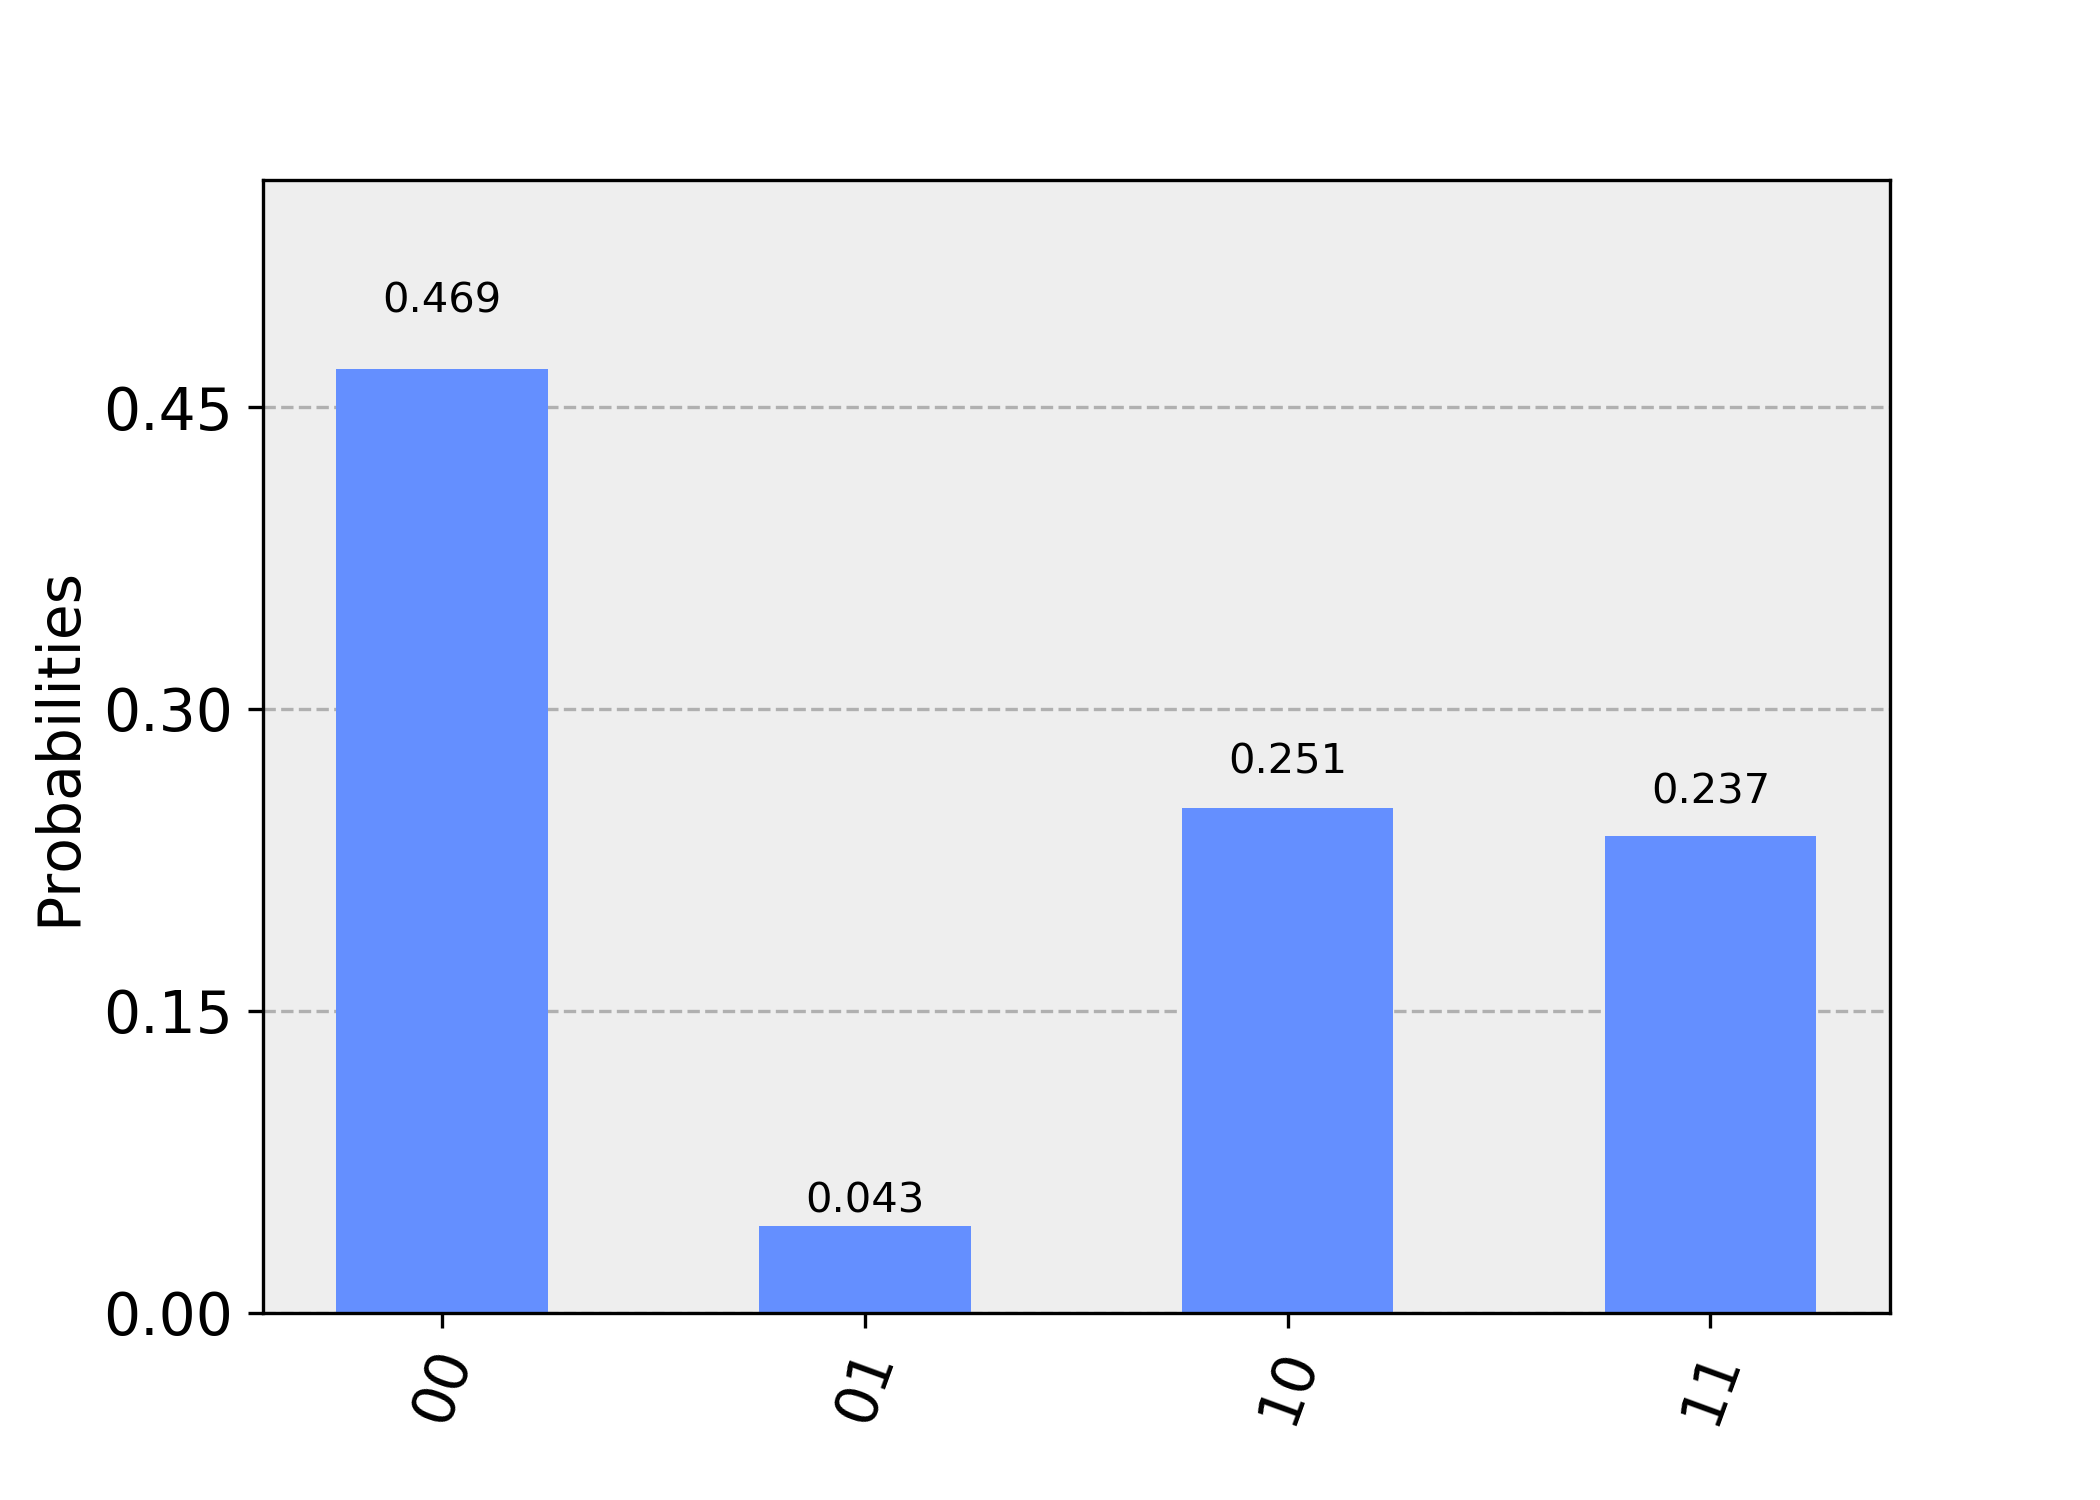
\includegraphics[width=\linewidth]{gfx/misura_setosa}
    } \\
    \subfloat[Iris versicolor] {
        \label{fig:misura_versicolor}
        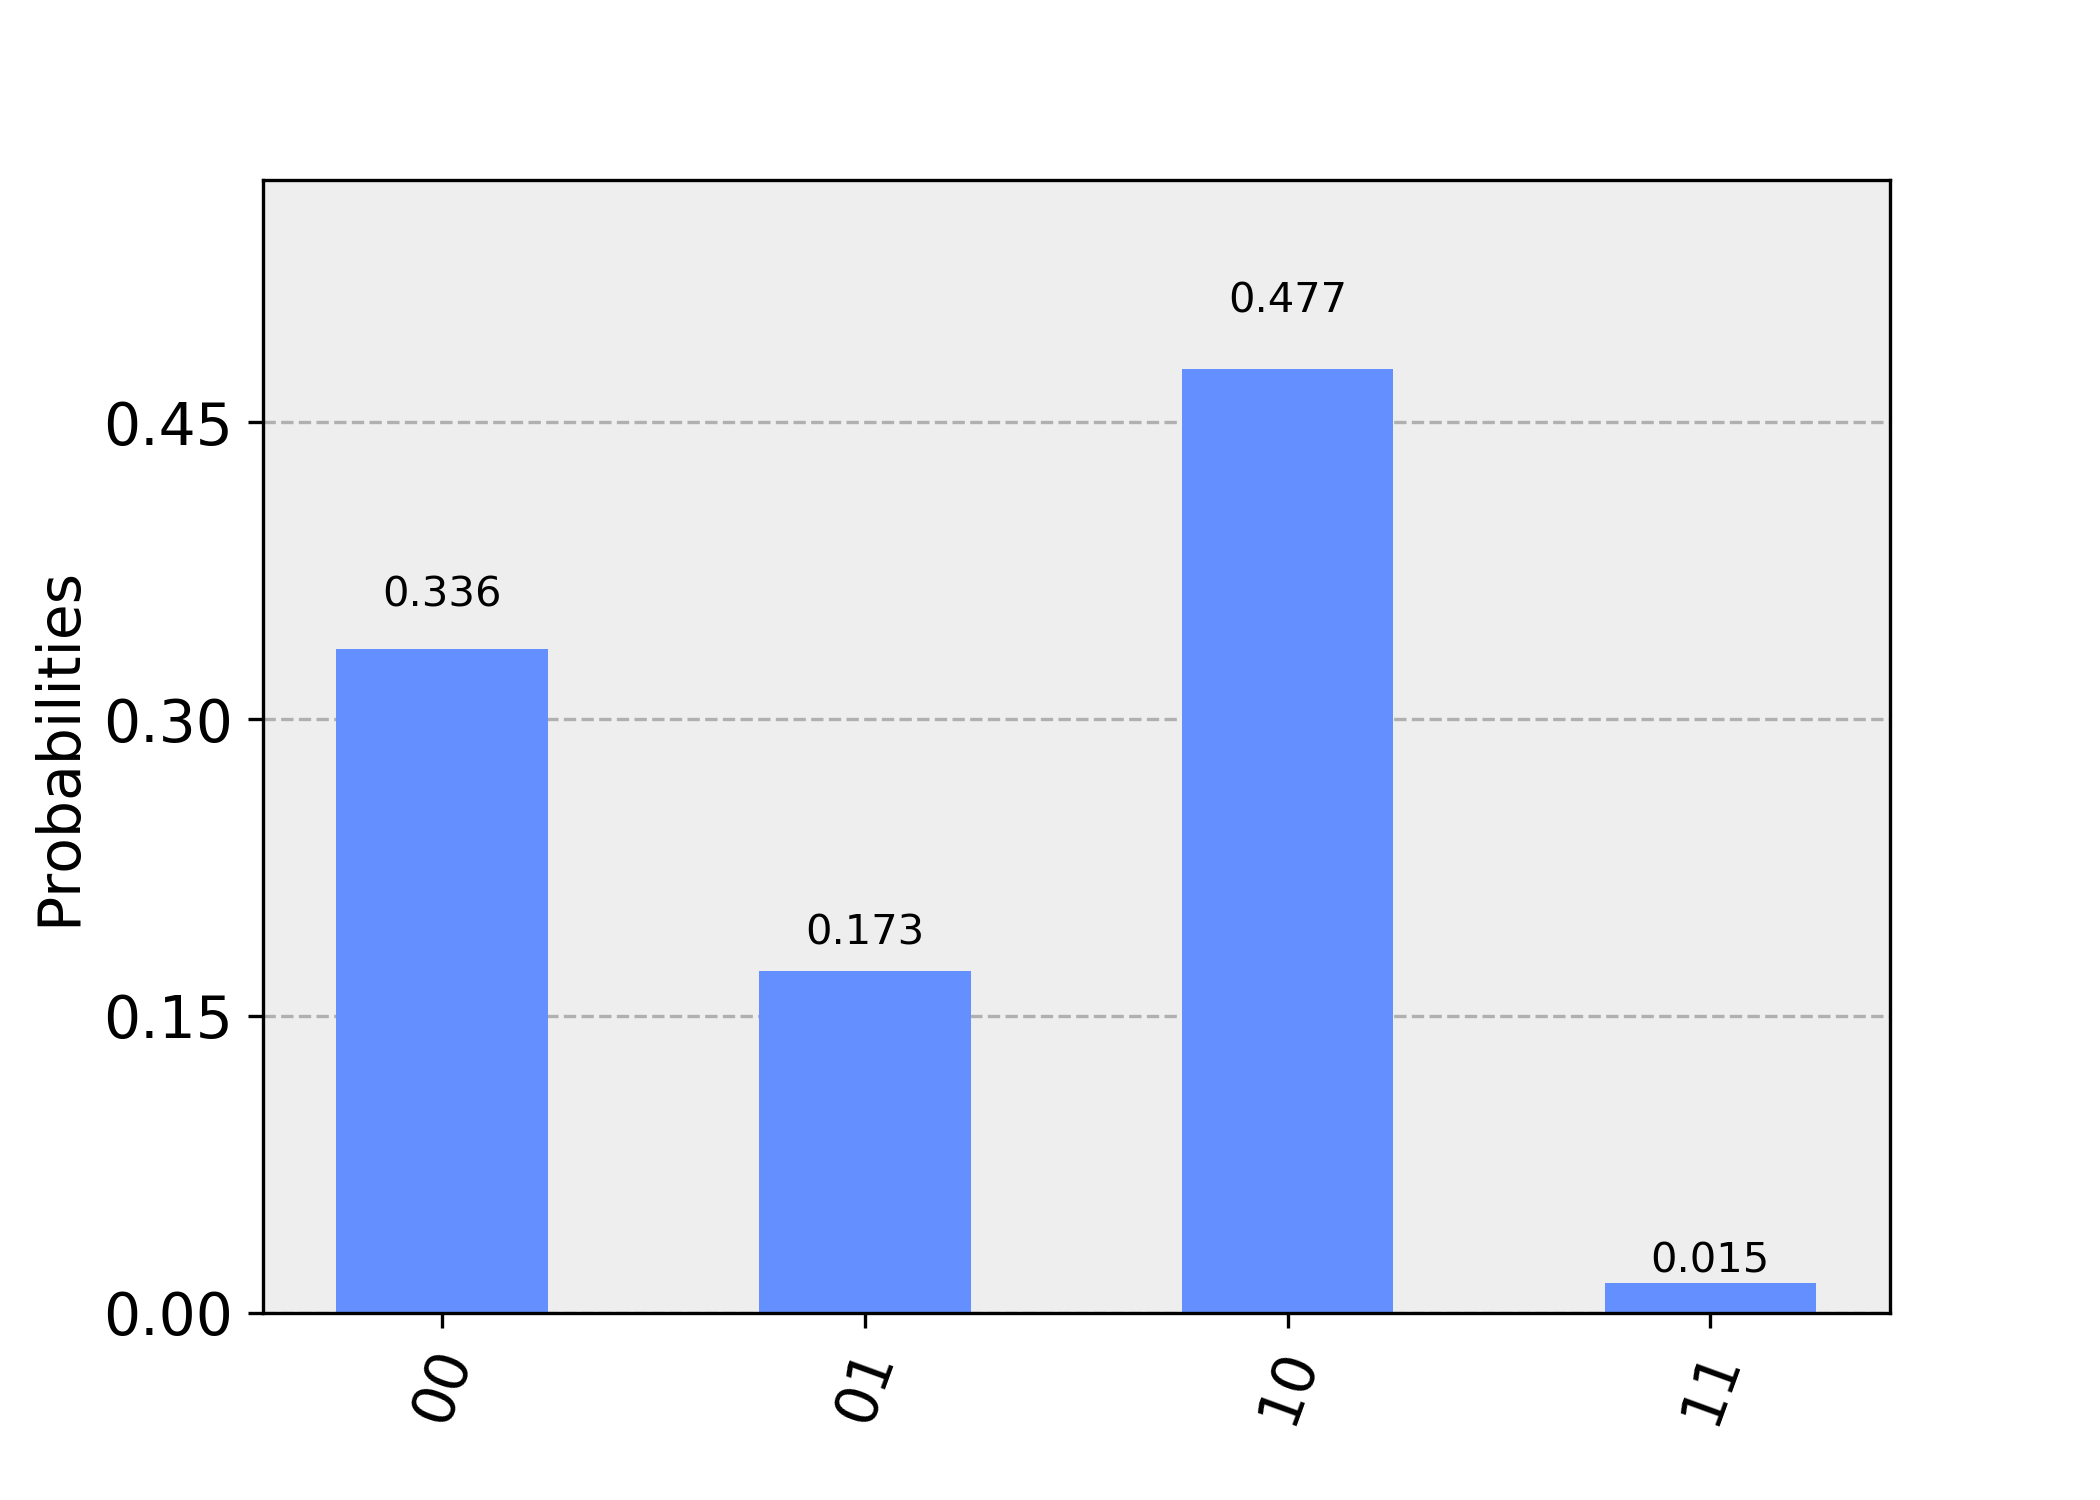
\includegraphics[width=\linewidth]{gfx/misura_versicolor}
    }
    \caption[Simulazione del circuito]%
    {Simulazione del circuito. \par \small 
    I conteggi totali sono: \\
    per setosa \{'00': 3843, '10': 2056, '01': 352, '11': 1941\}; \\
    per versicolor \{'00': 2749, '10': 3908, '01': 1414, '11': 121\}.}
    \label{fig:simulazione_circuito}
\end{figure}
Selezionando i risultati laddove il bit di destra è 0, abbiamo praticamente effettuato 
la misura condizionale necessaria al funzionamento dell'algoritmo. 
Nel riquadro \ref{fig:simulazione_filtrati} sono presentati 
i risultati filtrati in modo da considerare solo i risultati in cui il bit 
ancilla è 0. 
\begin{figure}[h!]
    \myfloatalign
    \subfloat[Iris setosa]{
        \label{fig:misura_setosa_filtrata}
        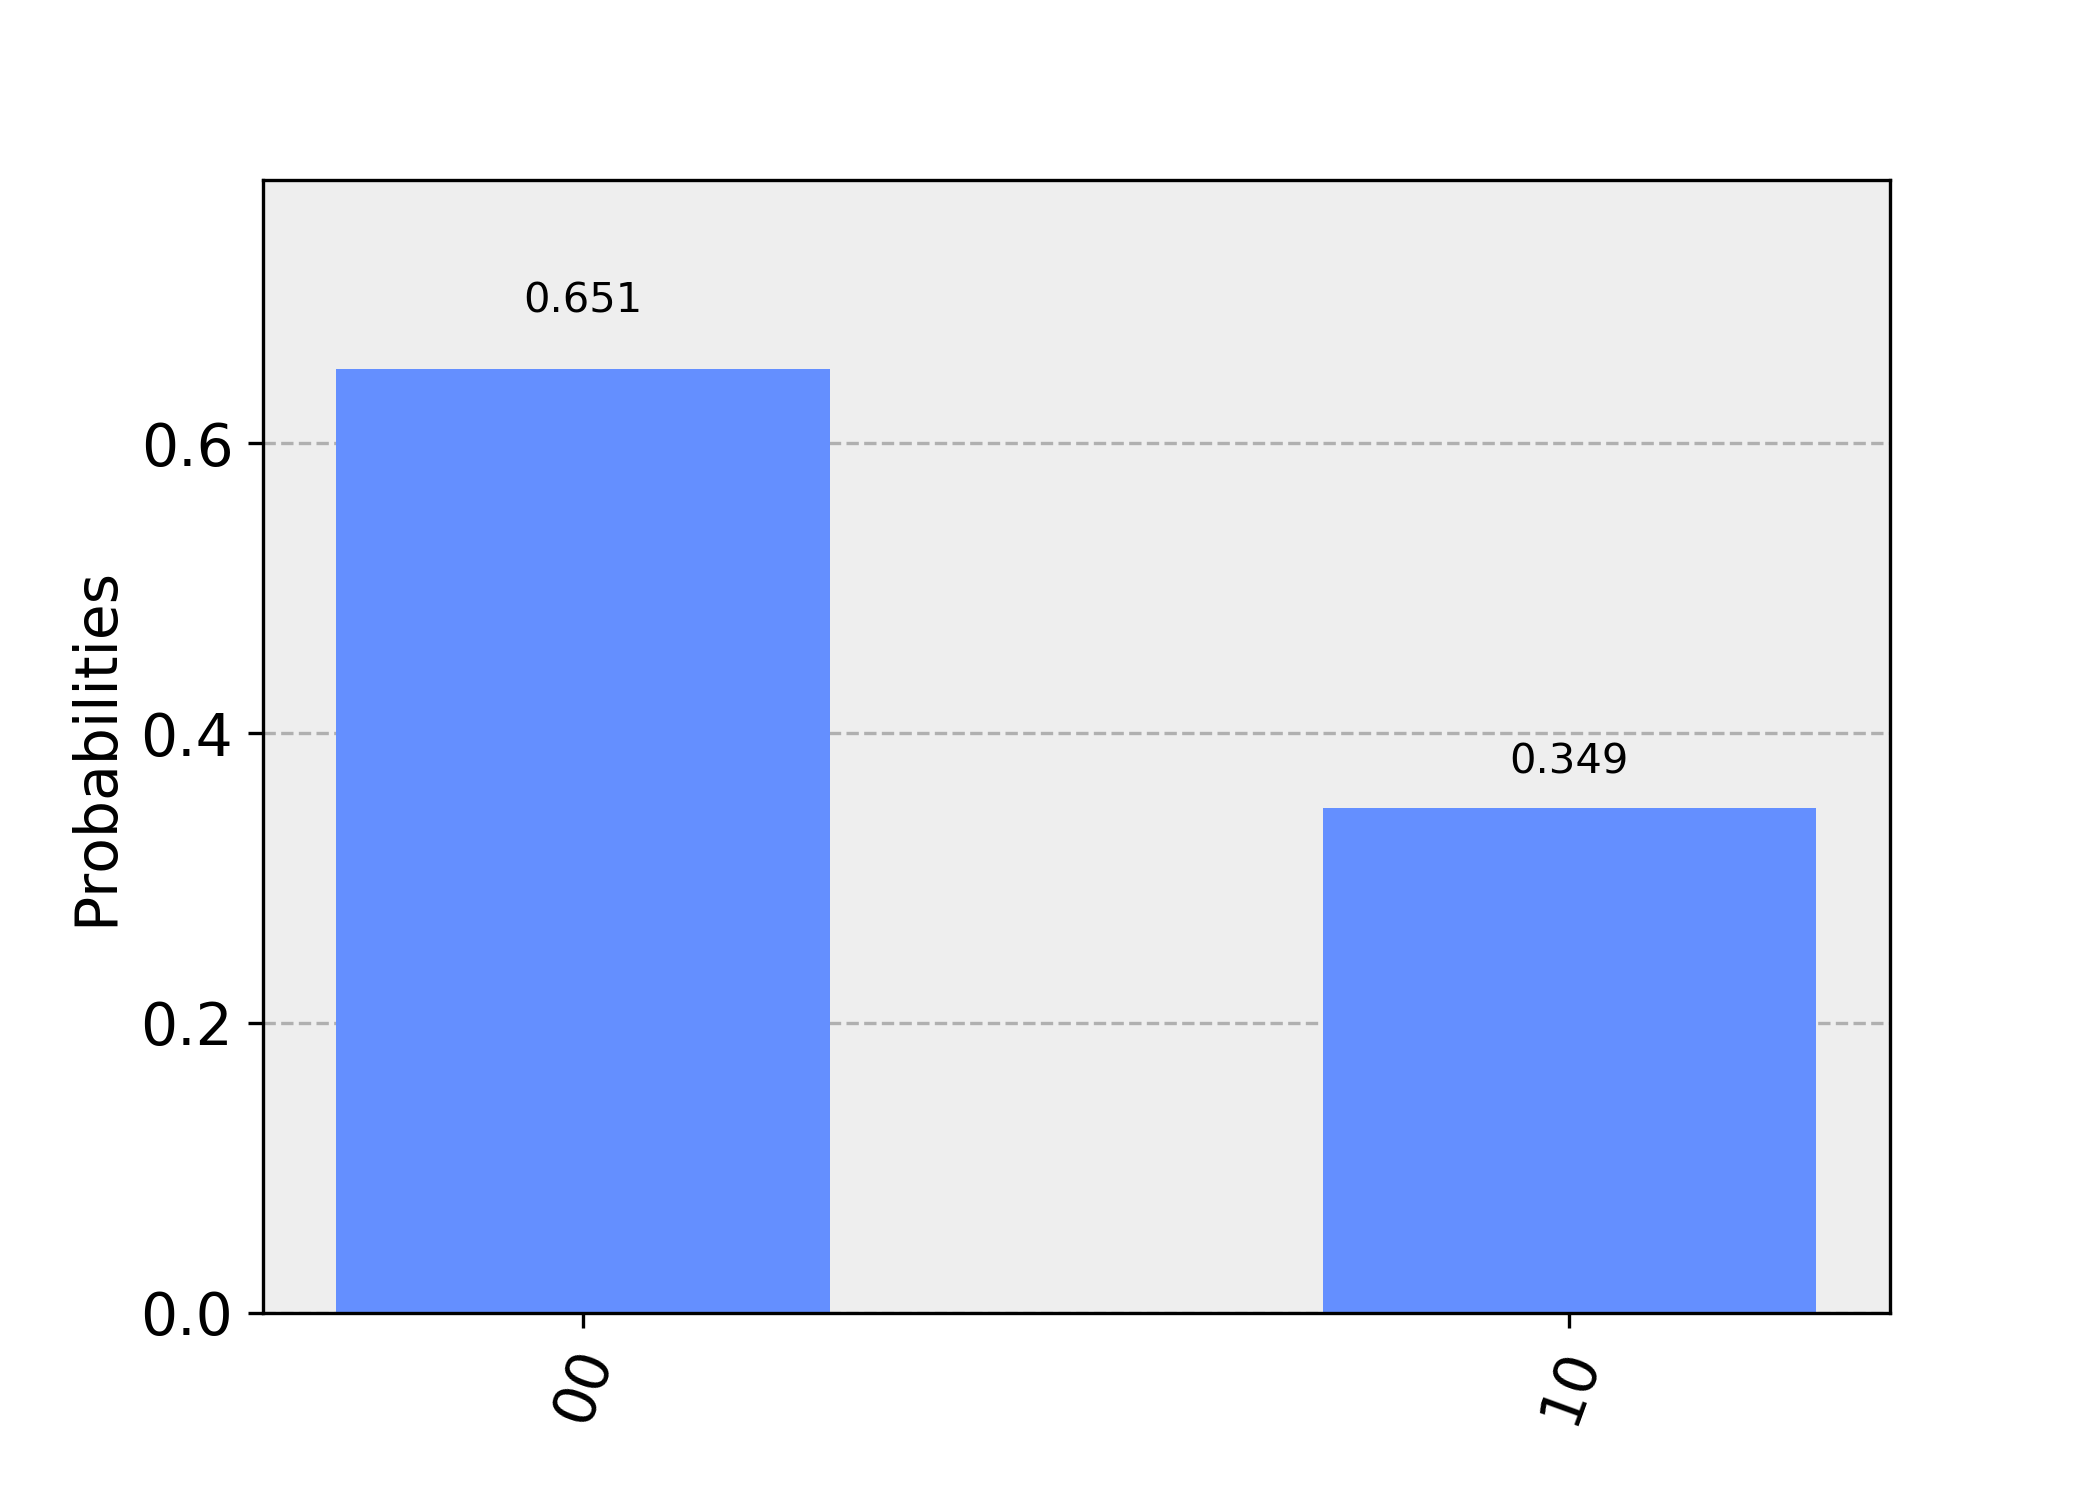
\includegraphics[width=\linewidth]{gfx/misura_setosa_filtrata}
    } \\
    \subfloat[Iris versicolor]{
        \label{fig:misura_versicolor_filtrata}
        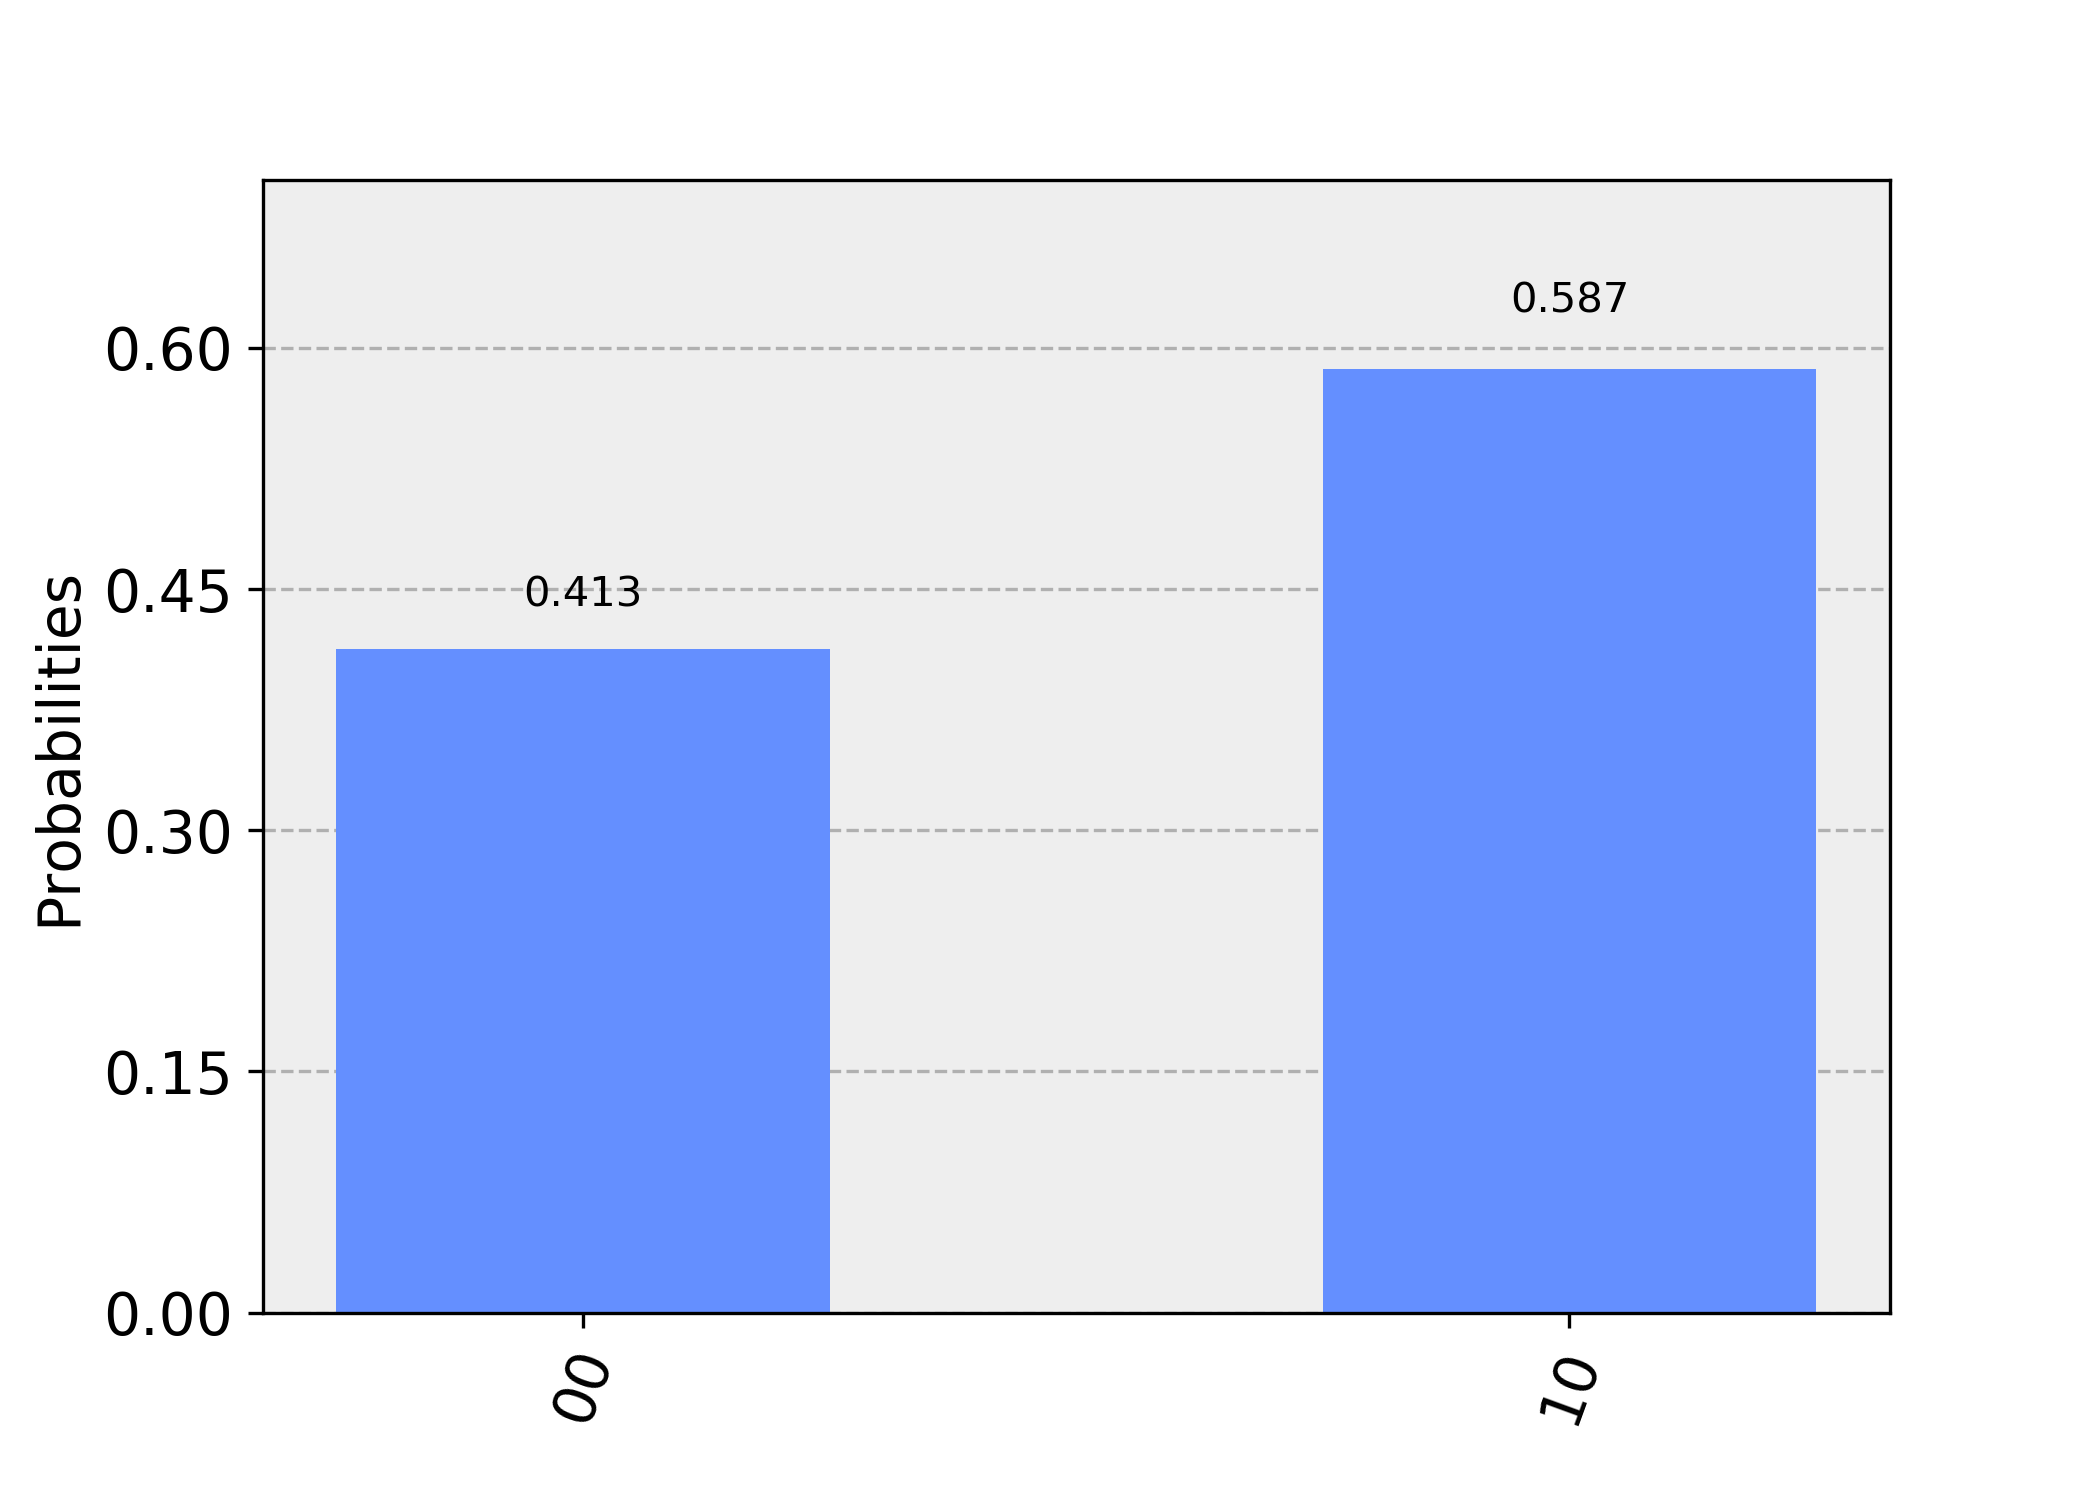
\includegraphics[width=\linewidth]{gfx/misura_versicolor_filtrata}
    }
    \caption{Simulazione del circuito, risultati filtrati}
    \label{fig:simulazione_filtrati}
\end{figure}

Il passo successivo è eseguire questi stessi circuiti quantistici su un vero computer quantistico. 
È stata scelta la macchina a 16 qubit ibmq\_16\_melbourne per ottenere le misure per il 
vettore d'input setosa illustrate in figura \ref{fig:sperimentale_setosa}. 
\begin{figure}[h!]
    \centering
    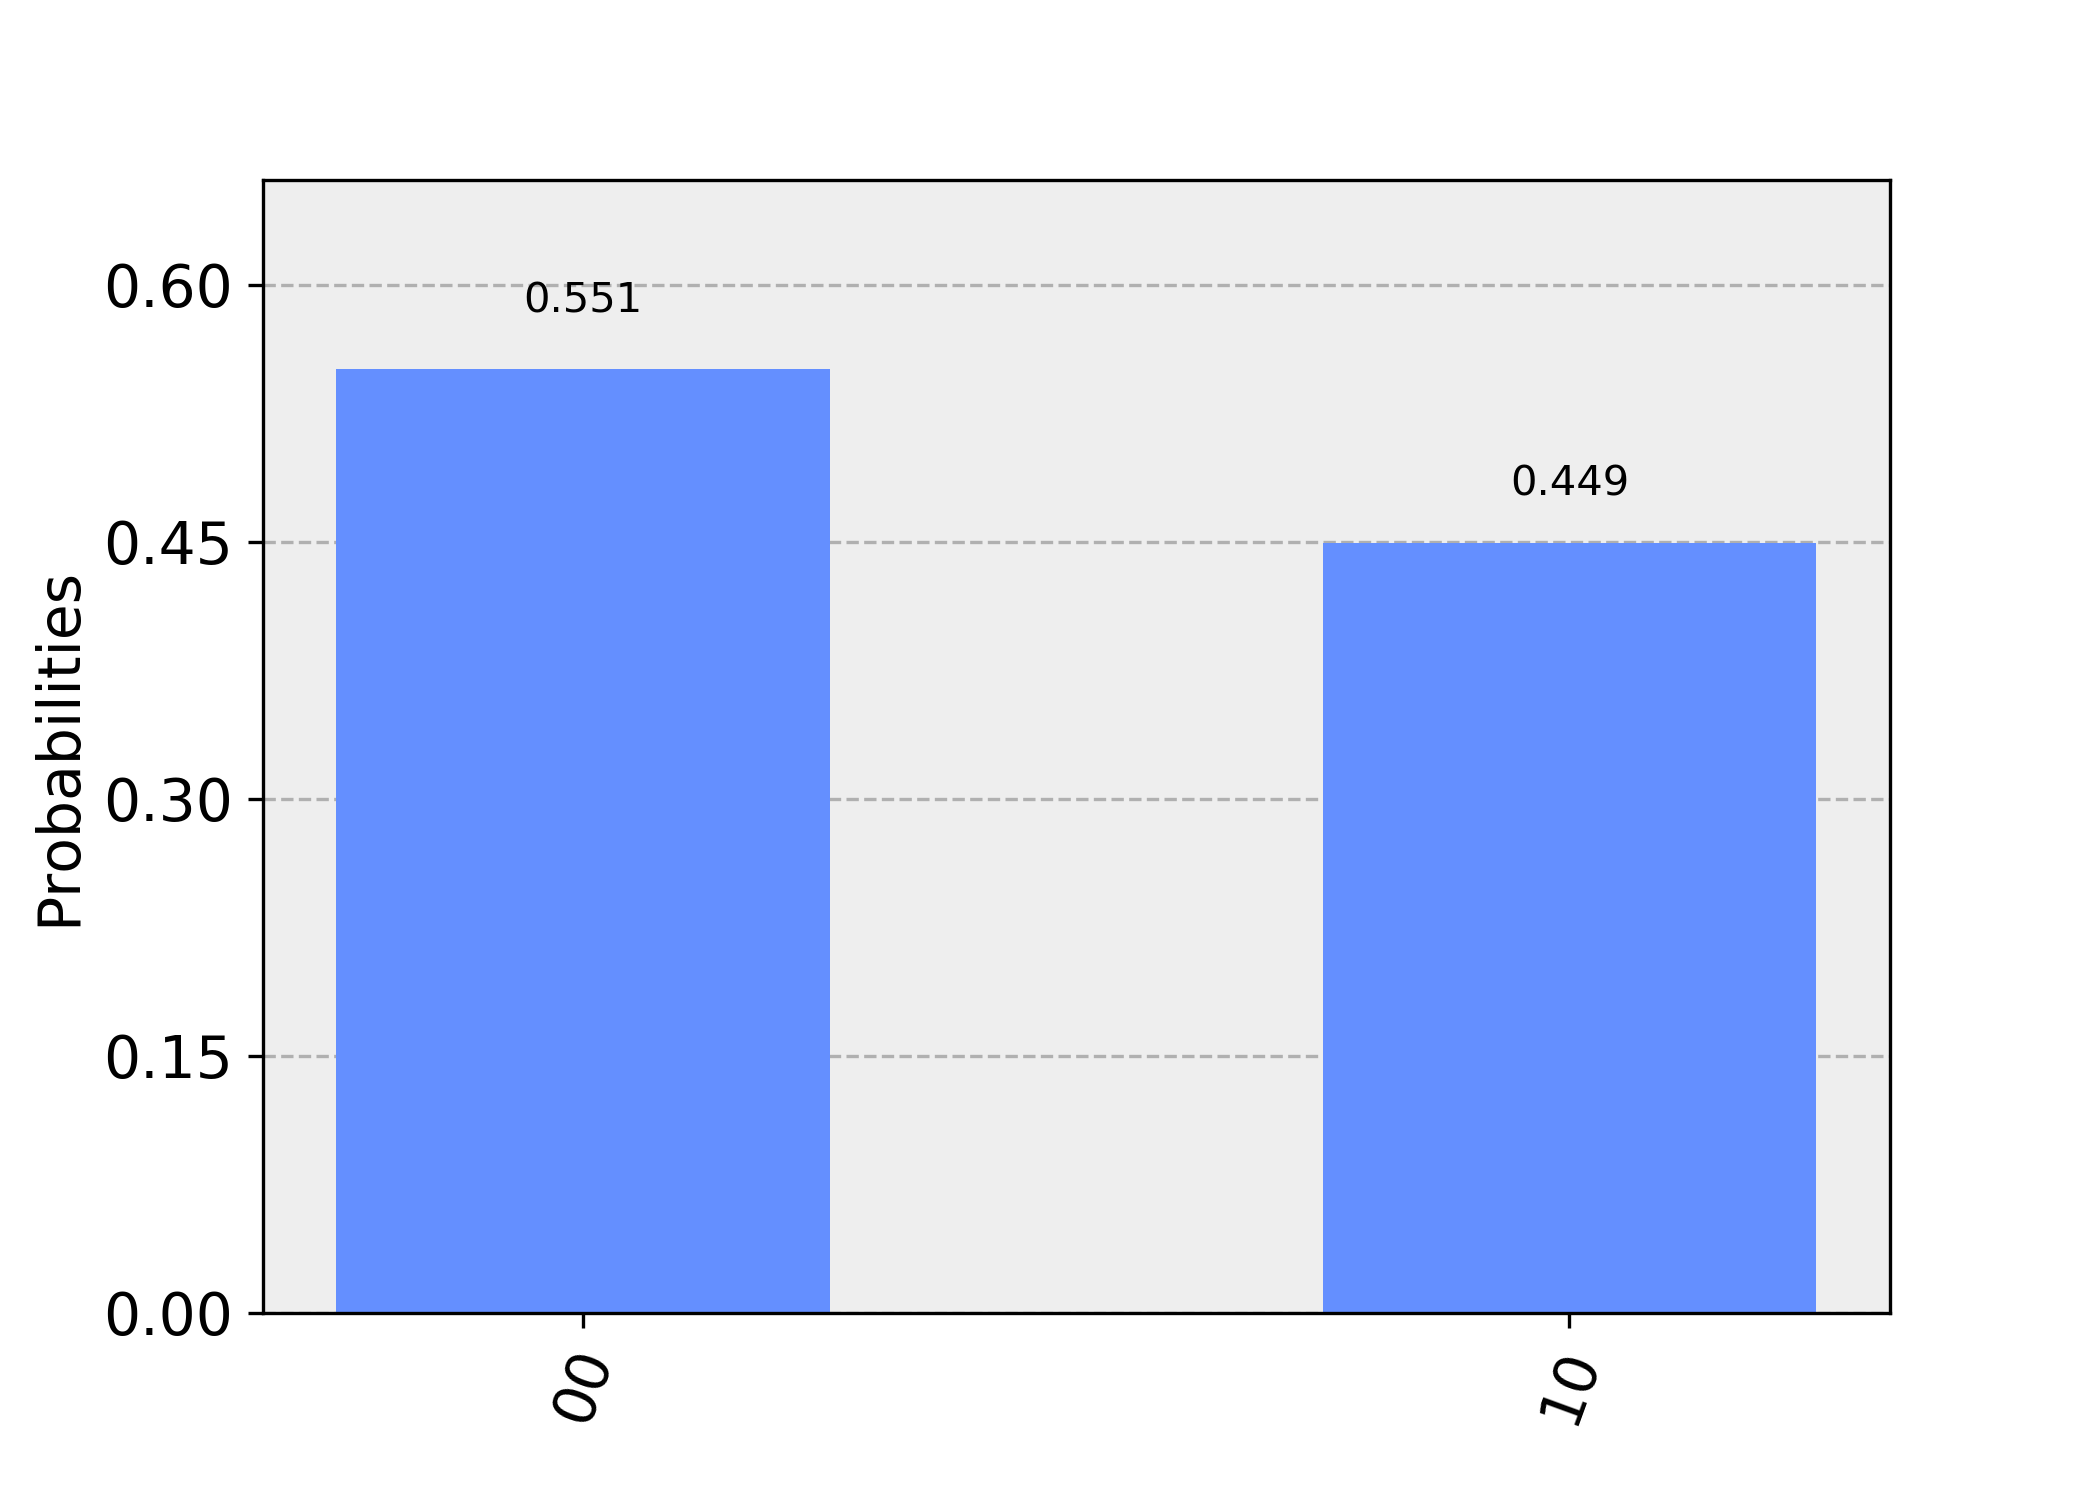
\includegraphics[width=\linewidth]{gfx/misura_setosa_sperimentale}
    \caption{Esecuzione su hardware reale (setosa)}
    \label{fig:sperimentale_setosa}
\end{figure}
Gli inevitabili fenomeni di rumore rendono i risultati meno piccati ma comunque 
distinguibili in questo caso. 

Il discorso è diverso per il confronto tra le classi versicolor e 
virginica: visto che gli elementi di queste due classi non sono linearmente separabili, 
algoritmi come quello qui usato non sono efficaci nella loro distinzione. 
Uno dei metodi per aggirare questo problema è l'uso di feature map \cite{schuld} nel processo 
di ottimizzazione. Infatti le misure effettuate danno risultati erronei o 
ambigui nella maggioranza dei casi (probabilità del 50\% per entrambi i risultati). 

Ad ogni modo, si procederà nel realizzare i punti definiti all'inizio di 
questo capitolo. Condizione necessaria per distinguere le tre classi con un 
solo esperimento è che si possano memorizzare almeno tre vettori di training, 
uno per ciascuna classe. 

\subsection{Aumento del numero di vettori d'apprendimento}

Il numero di stati posseduti da $n$ qubit, come abbiamo visto nella 
sezione sui fondamenti teorici, è $2^n$. Nell'esperimento visto poco 
prima, si è dedicato un solo qubit per segnare l'indice dei vettori di 
apprendimento $\ket{m}$. Aggiungendo ulteriori qubit all'indice possiamo 
immagazzinare successivamente 4, 8, 16, 32, 64, \ldots vettori di training. 
Con 8 qubit per il registro $\ket{m}$ già siamo in grado di immagazzinare 
tutti i vettori del data set Iris. Nel caso di grandi insiemi, tuttavia, 
potrebbe essere appropriato ridurre il numero di vettori di training durante 
il processo di ottimizzazione, adottando un criterio di selezione che includa 
solo i vettori più significativi ai fini della classificazione. 

La spesa totale in termini di risorse coinvolge due qubit per ogni incremento 
che facciamo: infatti, per mettere in entanglement un qubit in più del registro 
$\ket{m}$ con il qubit registro della \ac{QRAM}, abbiamo bisogno di un qubit 
ancilla aggiuntivo per l'operazione $C^n R_y (\theta)$; questi qubit ancilla non 
sono rappresentati nei disegni dei circuiti per semplice convenienza visiva, ma 
se ne può trovare traccia nei frammenti di codice scritti per questa tesi\footnote{Si veda 
\url{https://github.com/visika/Tesi}}.

\subsection{Implementazione multiclasse}

L'aggiunta della capacità di riconoscere tutte le tre classi in una sola esecuzione 
non è di natura differente dall'aggiungere qubit per avere maggiori vettori 
di apprendimento. Passiamo dall'avere un solo qubit classe, che ha associato il 
proprio stato $\ket{0}$ alla prima classe e lo stato $\ket{1}$ alla seconda, 
ad avere due qubit classe ed associare lo stato $\ket{00}$ alla prima classe, 
lo stato $\ket{01}$ alla seconda classe e lo stato $\ket{10}$ alla terza classe. 
Lo stato $\ket{11}$ non è associato ad alcuna classe. 
Nel processo di costruzione dello stato iniziale nella \ac{QRAM}, 
oltre che ai qubit indice, i vettori di addestramento saranno in entanglement 
anche con i relativi stati dei due qubit classe. Osservando la figura \ref{fig:qram_classi} 
si vede che le porte $\overline{c}X$ sui qubit classe sono applicate solo all'inizio e 
alla fine del processo di codifica di tutte le componenti di un vettore di training. 
\begin{figure}[h!]
    \centering
    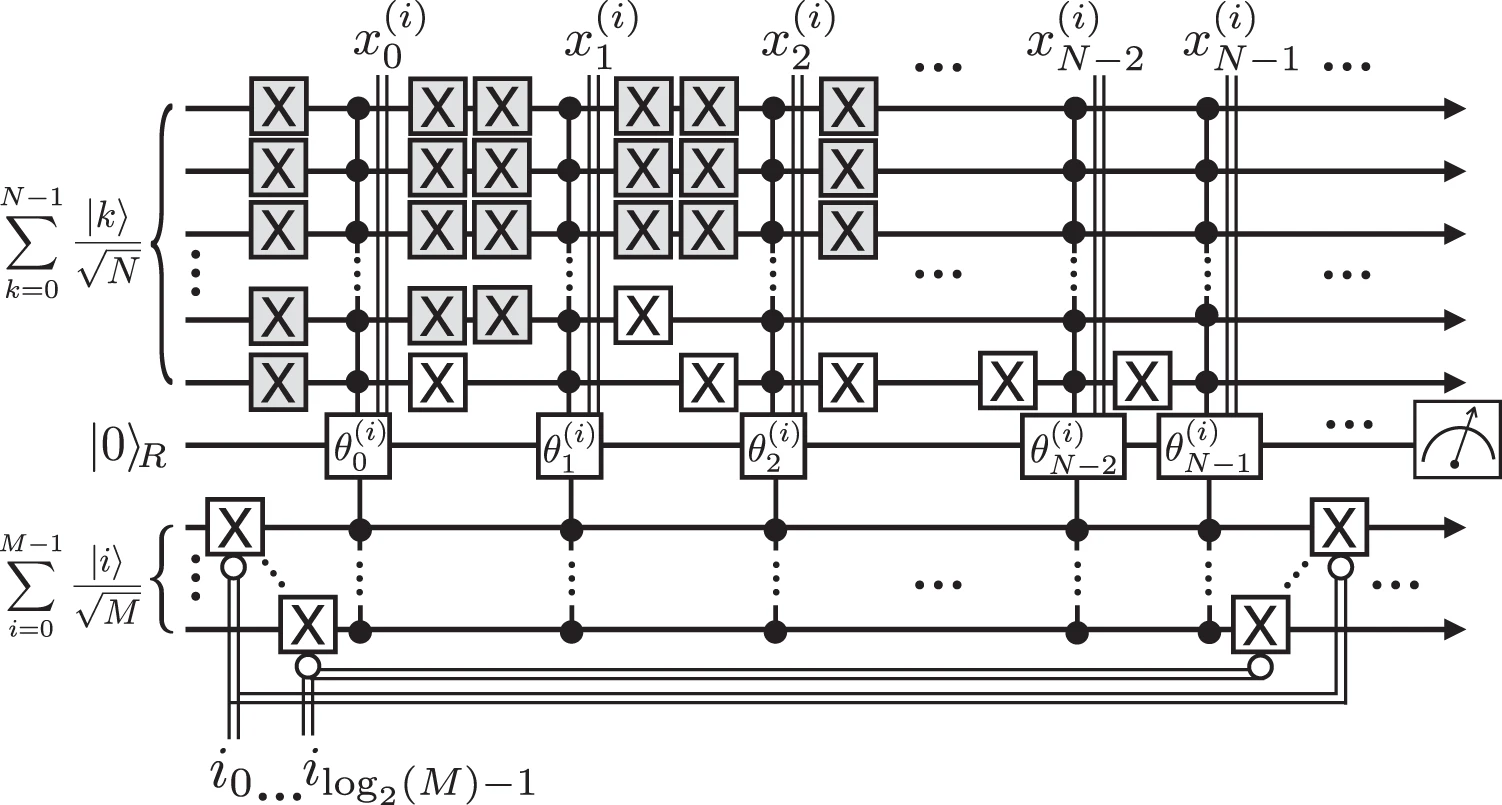
\includegraphics[width=\linewidth]{gfx/qram_classi}
    \caption[Circuito quantistico per preparare il \acs{QDB} per un quantum support vector machine]%
    {Circuito quantistico per preparare il \acs{QDB} per un quantum support vector machine. \par \small 
    Sono mostrate le porte per scrivere solo l'$i$-esimo vettore di apprendimento. Le porte ombreggiate 
    in grigio sono aggiunte esclusivamente per illustrare il processo flip-flop, e non sono implementate 
    in pratica.}
    \label{fig:qram_classi}
\end{figure}

\subsection{Aumento del numero di caratteristiche}

% *********************************************
% Questa parte va aggiustata
% *********************************************

L'Iris data set possiede 4 caratteristiche. È poco dispendioso includerle tutte 
dunque usando semplicemente 2 qubit $\ket{i}$ e 2 qubit come ancilla della \ac{QRAM}. 
Per verificare il miglioramento apportato da un aumento del numero di caratteristiche 
considerate, si prende in esame la classificazione del vettore d'input 54 (versicolor), 
con i vettori di training numero 51 (versicolor) e 146 (virginica) del data set. 
Il vettore d'input viene classificato correttamente durante la simulazione con due caratteristiche, 
con probabilità vicina al 51.4\%. 
Effettuando la stessa misura, ma tenendo conto di tutte le quattro feature, arriviamo ad 
una probabilità di classificazione corretta del 58.3\% nel migliore dei casi. 
Sembra esserci un margine di miglioramento in determinati casi, 
ma non può essere garantito in maniera generale. 

\section{Esecuzione completa}

Per studiare l'efficienza dell'algoritmo a diversi stadi di miglioramento, 
si divide il data set in un insieme dedicato all'addestramento ed un insieme 
di vettori da classificare. Al fine di avere risultati imparziali, 
per ogni esecuzione i vettori di training ed il vettore d'input 
sono scelti casualmente a partire dal data set completo. 
Si contano le classificazioni di successo 
rispetto al totale dei tentativi, al variare dei parametri come il numero 
di features o il numero di vettori di training usati. 

Provando ad effettuare una classificazione a tre classi con 32 vettori di 
training otteniamo i seguenti esiti: 
\begin{itemize}
    \item i vettori della classe setosa sono correttamente classificati 10 volte su 10;
    \item i vettori della classe versicolor sono correttamente classificati 5 volte su 10;
    \item i vettori della classe virginica sono correttamente clasificati 9 volte su 10.
\end{itemize}
I risultati vengono necessariamente da simulazioni, in quanto sono necessari 
19 qubit sotto queste condizioni. 

Volendo sfruttare appieno le potenzialità del simulatore presso l'IBM, 
possiamo costruire un circuito che accetti $2^7 = 128$ vettori di training 
presi a caso, e lasciare i restanti vettori per la classificazione. 
Con l'uso di 23 qubit si arriva alla classificazione corretta della classe versicolor 
8 volte su 10. 
%************************************************
\chapter{Conclusione}\label{ch:conclusione}
%************************************************

Partendo da un semplice classificatore \ac{KNN} classico 
si è riusciti ad implementarne la versione quantistica proposta 
da Schuld et al. \cite{schuld}. Dopo di che si è tentato di 
estenderne le funzioni, con l'intento principale di rendere il 
classificatore capace di distinguere la classe corretta tra 
tutte quelle dell'insieme dati e non solo per due alla volta. 
È stata usata la tecnica di 
costruzione di quantum database arbitrari \ac{FF-QRAM} proposta da 
Petruccione et al. \cite{petruccione}. L'algoritmo ha avuto un 
discreto successo e fornisce una distribuzione di previsioni 
in linea con le aspettative, sebbene le esecuzioni su hardware 
reale siano ancora significativamente in balia dei fenomeni di 
rumore. L'avvento di computer quantistici con un numero maggiore 
di qubit può aprire la strada ad approcci concreti di analisi 
dati con data set di dimensioni e complessità considerevoli, 
lasciando intravedere un'opportunità di applicazione 
commerciale nei confronti dei big data. 

Per questioni di limitatezza di tempo, non è stato possibile 
sottoporre ad analisi anche altri data set o implementare tecniche 
più raffinate di preprocessing dei dati. Il lettore interessato 
ad approfondire la materia in maniera più sistematica si può 
affidare a lavori analoghi facilmente reperibili 
online\footnote{Si veda ad esempio 
\url{https://github.com/carstenblank/dc-qiskit-qml}.}, alla comunità 
di Qiskit su \url{https://quantumcomputing.stackexchange.com/} o ai tanti 
articoli sull'argomento che escono ogni anno in libera consultazione. 

Un'interessante proseguimento di questo progetto potrebbe essere 
la messa a disposizione degli algoritmi qui studiati per chi volesse 
usarli per analizzare data set personalizzati. Questo potrebbe 
essere realizzato attraverso un'ulteriore ottimizzazione e 
documentazione del codice pubblicato su GitHub, oppure con la 
creazione di un programma completo apposito, o ancora con la 
costruzione di un'interfaccia web in cui caricare i propri file 
(CSV per esempio) e lasciare che il server ottimizzi i dati, crei 
il circuito quantistico e mandi l'ordine di esecuzione correlato. 

\section{Commento}

Lavorare a questa tesi mi ha permesso di esplorare le terre, 
del machine learning e del quantum computing, due materie 
fortemente moderne ed in continua evoluzione. 
Nonostante l'approfondimento delle materie compiuto in 
questi mesi di lavoro sia tutt'altro che completo, 
mi ritengo soddisfatto di essere riuscito a mettere a frutto 
le mie pregresse conoscenze di informatica per partecipare a 
qualcosa di estremamente innovativo. La critica che faccio a 
me stesso è di avere iniziato a scrivere ben troppo tardi il 
testo della tesi; se dovessi ripetere questa esperienza, 
cercherei di fissare bene fin dall'inizio gli obiettivi di 
ricerca e tenere traccia dei progressi in maniera più assidua, 
aggiornando in corso d'opera il documento finale. 
%\addtocontents{toc}{\protect\clearpage} % <--- just debug stuff, ignore
%\include{multiToC} % <--- just debug stuff, ignore for your documents
% ********************************************************************
% Backmatter
%*******************************************************
\appendix
%\renewcommand{\thechapter}{\alph{chapter}}
\cleardoublepage
\part{Appendice}
%********************************************************************
% Appendice
%*******************************************************
% If problems with the headers: get headings in appendix etc. right
%\markboth{\spacedlowsmallcaps{Appendix}}{\spacedlowsmallcaps{Appendix}}
\chapter{Appendice}

\begin{figure}[ht]
    \hspace{-2.5cm}
    \begin{adjustbox}{addcode={\begin{minipage}{\width}}{\caption{
        Il circuito quantistico. 
        }\end{minipage}},rotate=90,center}
        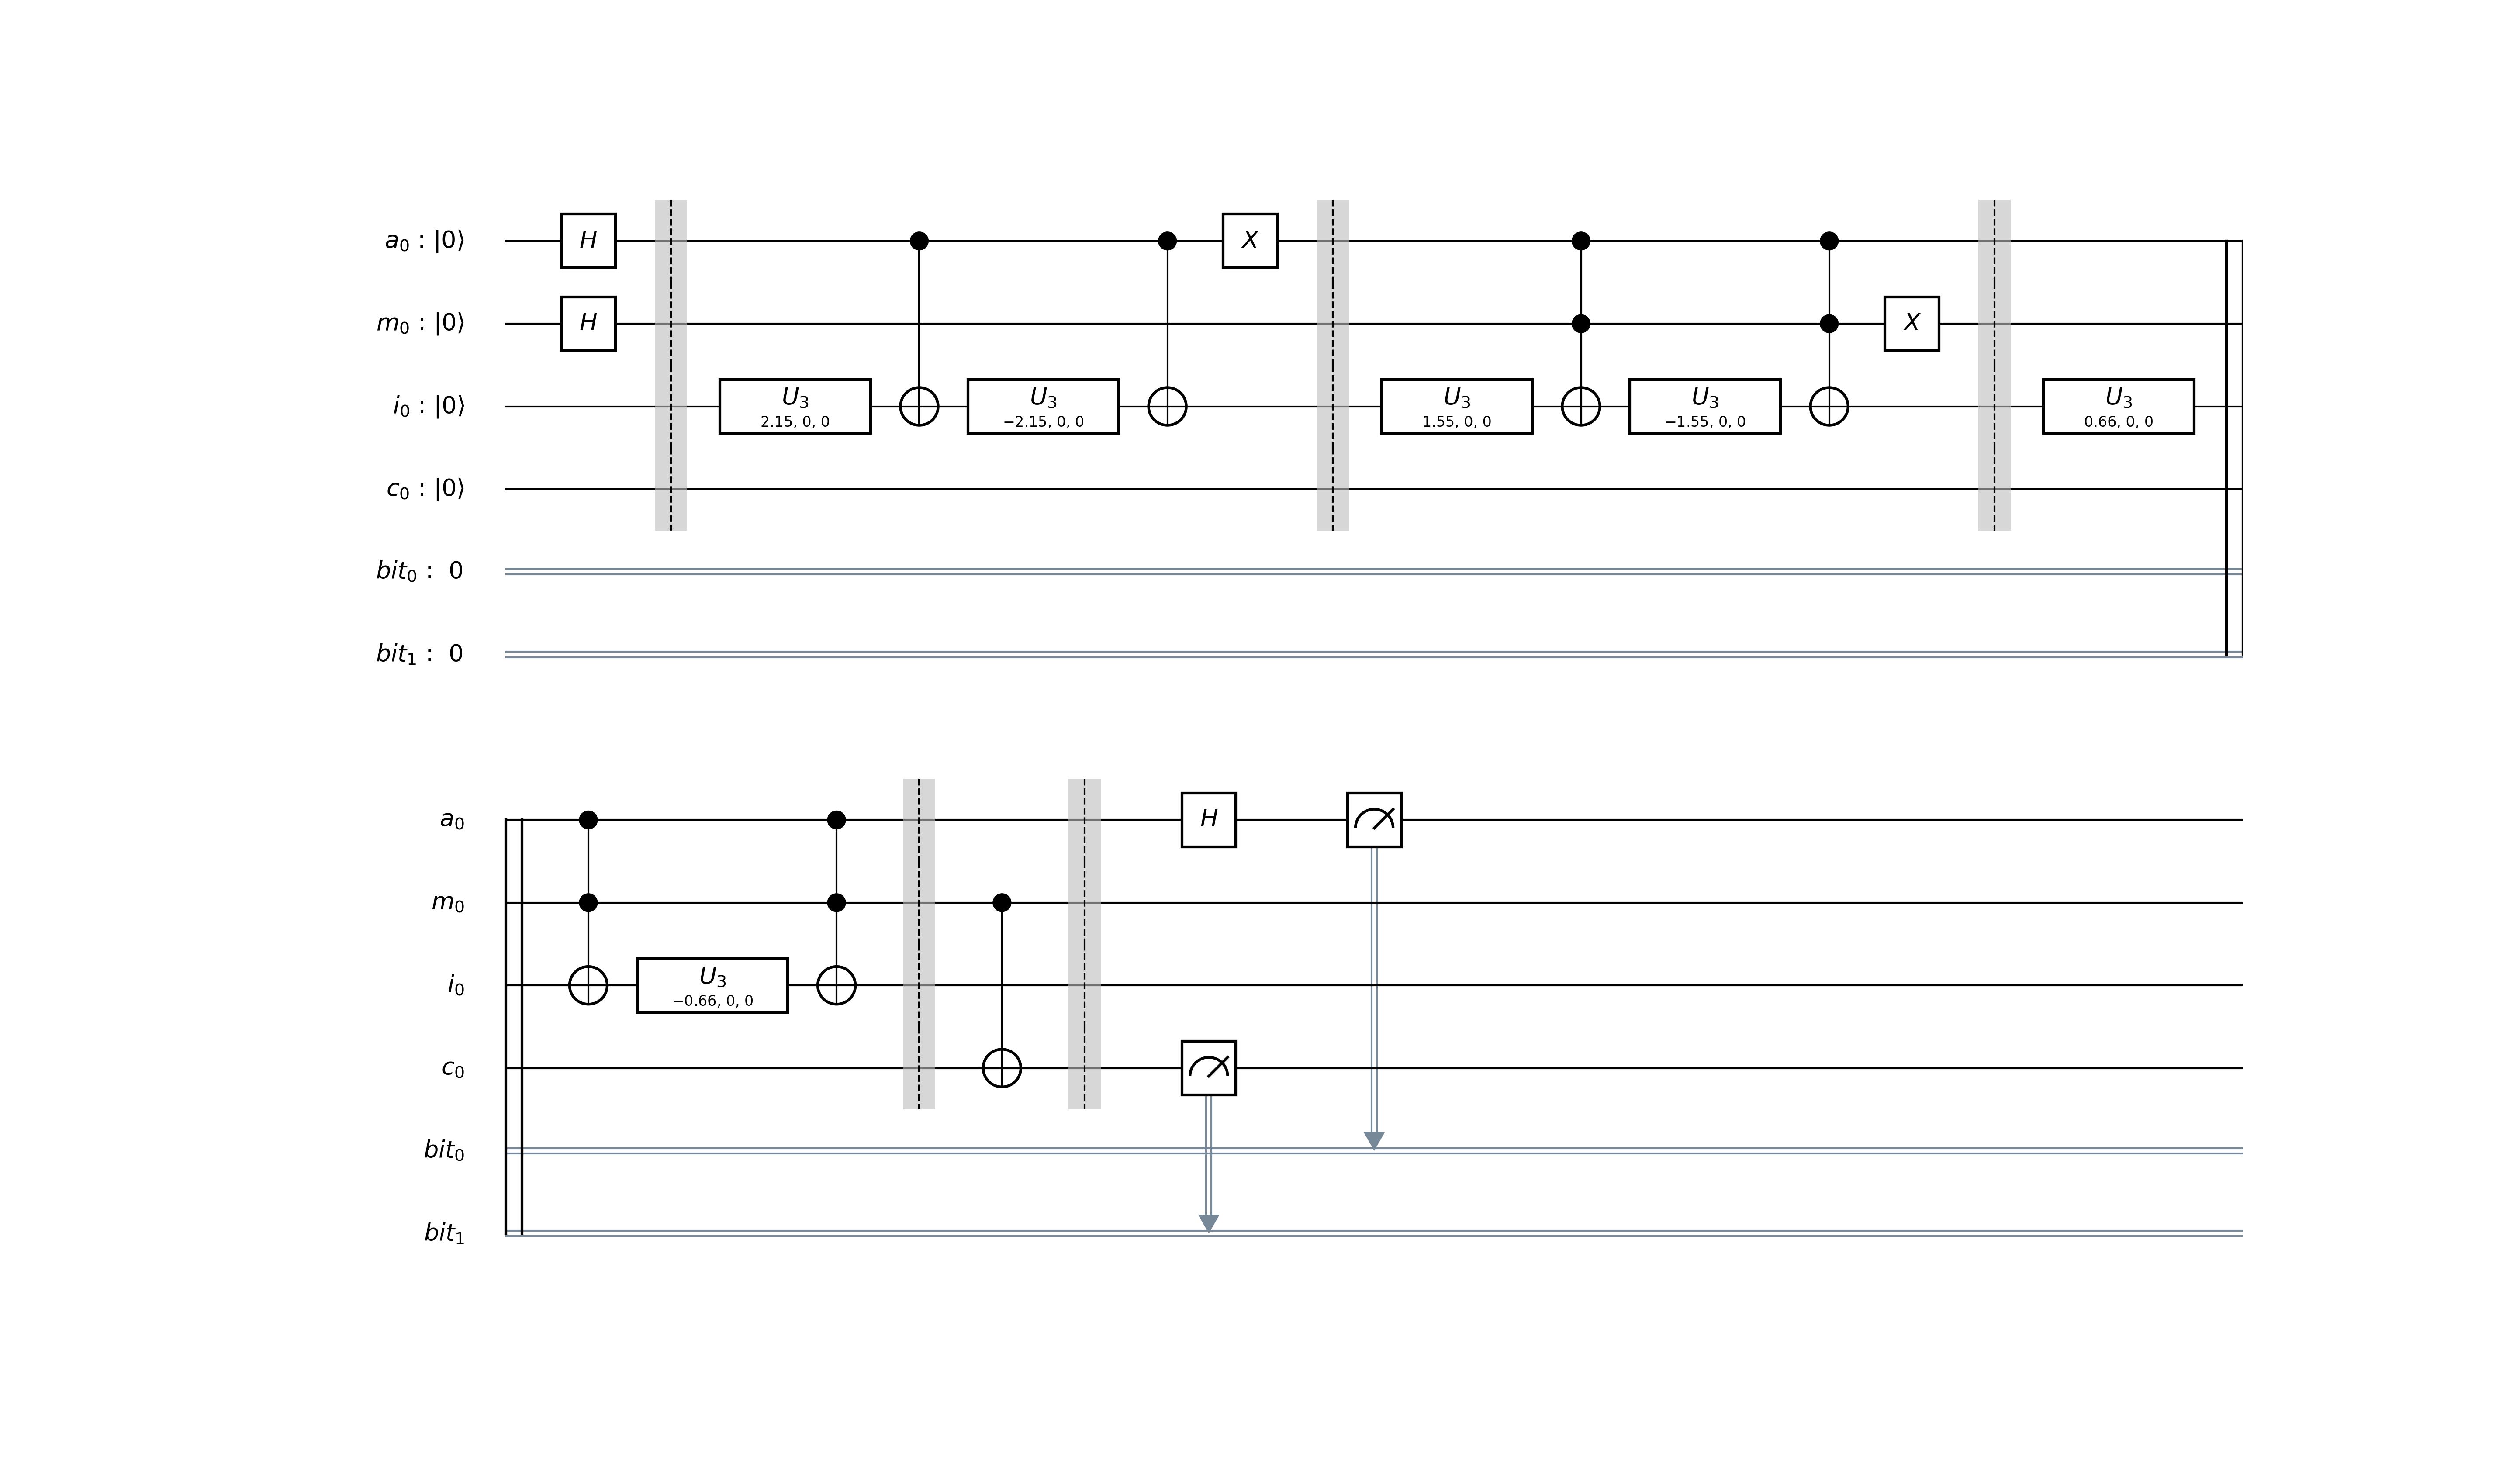
\includegraphics[scale=0.5]{gfx/base_circuit}
    \end{adjustbox}
\label{fig:circuitoquantistico}
\end{figure}
%********************************************************************
% Other Stuff in the Back
%*******************************************************
\cleardoublepage%********************************************************************
% Bibliography
%*******************************************************
% work-around to have small caps also here in the headline
% https://tex.stackexchange.com/questions/188126/wrong-header-in-bibliography-classicthesis
% Thanks to Enrico Gregorio
\defbibheading{bibintoc}[\bibname]{%
  \phantomsection
  \manualmark
  \markboth{\spacedlowsmallcaps{#1}}{\spacedlowsmallcaps{#1}}%
  \addtocontents{toc}{\protect\vspace{\beforebibskip}}%
  \addcontentsline{toc}{chapter}{\tocEntry{#1}}%
  \chapter*{#1}%
}
\printbibliography[heading=bibintoc]

% Old version, will be removed later
% work-around to have small caps also here in the headline
%\manualmark
%\markboth{\spacedlowsmallcaps{\bibname}}{\spacedlowsmallcaps{\bibname}} % work-around to have small caps also
%\phantomsection
%\refstepcounter{dummy}
%\addtocontents{toc}{\protect\vspace{\beforebibskip}} % to have the bib a bit from the rest in the toc
%\addcontentsline{toc}{chapter}{\tocEntry{\bibname}}
%\label{app:bibliography}
%\printbibliography

% \cleardoublepage%*******************************************************
% Declaration
%*******************************************************
\pdfbookmark[0]{Declaration}{declaration}
\chapter*{Declaration}
\thispagestyle{empty}
Put your declaration here.
\bigskip

\noindent\textit{\myLocation, \myTime}

\smallskip

\begin{flushright}
    \begin{tabular}{m{5cm}}
        \\ \hline
        \centering\myName \\
    \end{tabular}
\end{flushright}

\cleardoublepage\pagestyle{empty}

\hfill

\vfill


\pdfbookmark[0]{Colophon}{colophon}
\section*{Colophon}
Questo documento è stato composto usando il tema tipografico \texttt{classicthesis} sviluppato da Andr\'e Miede e Ivo Pletikosić.
Lo stile trae ispirazione dal libro fondamentale sulla tipografia ``\emph{The Elements of Typographic Style}'' di Robert Bringhurst.
\texttt{classicthesis} è disponibile per \LaTeX\ e \mLyX:
\begin{center}
\url{https://bitbucket.org/amiede/classicthesis/}
\end{center}
Gli utenti soddisfatti di \texttt{classicthesis} di solito inviano una cartolina all'autore; 
una collezione di cartoline ricevute fin ora è esposta qui: 
\begin{center}
\url{http://postcards.miede.de/}
\end{center}
Grazie mille per il tuo riscontro e contributo. 

\bigskip

\noindent\finalVersionString

%Hermann Zapf's \emph{Palatino} and \emph{Euler} type faces (Type~1 PostScript fonts \emph{URW
%Palladio L} and \emph{FPL}) are used. The ``typewriter'' text is typeset in \emph{Bera Mono},
%originally developed by Bitstream, Inc. as ``Bitstream Vera''. (Type~1 PostScript fonts were made
%available by Malte Rosenau and
%Ulrich Dirr.)

%\paragraph{note:} The custom size of the textblock was calculated
%using the directions given by Mr. Bringhurst (pages 26--29 and
%175/176). 10~pt Palatino needs  133.21~pt for the string
%``abcdefghijklmnopqrstuvwxyz''. This yields a good line length between
%24--26~pc (288--312~pt). Using a ``\emph{double square textblock}''
%with a 1:2 ratio this results in a textblock of 312:624~pt (which
%includes the headline in this design). A good alternative would be the
%``\emph{golden section textblock}'' with a ratio of 1:1.62, here
%312:505.44~pt. For comparison, \texttt{DIV9} of the \texttt{typearea}
%package results in a line length of 389~pt (32.4~pc), which is by far
%too long. However, this information will only be of interest for
%hardcore pseudo-typographers like me.%
%
%To make your own calculations, use the following commands and look up
%the corresponding lengths in the book:
%\begin{verbatim}
%    \settowidth{\abcd}{abcdefghijklmnopqrstuvwxyz}
%    \the\abcd\ % prints the value of the length
%\end{verbatim}
%Please see the file \texttt{classicthesis.sty} for some precalculated
%values for Palatino and Minion.
%
%    \settowidth{\abcd}{abcdefghijklmnopqrstuvwxyz}
%    \the\abcd\ % prints the value of the length

% ********************************************************************
% Game Over: Restore, Restart, or Quit?
%*******************************************************
\end{document}
% ********************************************************************
